%%%%%%%%%%%%%%%%%%%%%%%%%%%%%%%%%%%%%%%%%%%%%%%%%%%%%%%%%%%%%%%%%%%%%%%%%%%%%%%
% Source Code of the 'GFDL Cloud Microphysics' Document
% Maintainer: Linjiong Zhou (linjiong.zhou@noaa.gov)
%%%%%%%%%%%%%%%%%%%%%%%%%%%%%%%%%%%%%%%%%%%%%%%%%%%%%%%%%%%%%%%%%%%%%%%%%%%%%%%

\documentclass[letterpaper,titlepage,10pt]{article}

\usepackage[margin=1in]{geometry}
\usepackage{natbib}
\usepackage{color}
\usepackage{bm}
\usepackage{graphicx}
\usepackage{amsmath}
\usepackage{diagbox}
%\usepackage{indentfirst}
\usepackage{natbib}
\PassOptionsToPackage{hyphens}{url}\usepackage{hyperref}
%\usepackage{hyperref}
\usepackage[titletoc,title]{appendix}
\usepackage{longtable}

\hypersetup{
	colorlinks=true,
	linkcolor=blue,
	filecolor=blue,
	urlcolor=blue,
	anchorcolor=blue,
	citecolor=blue,
}
 
\urlstyle{same}

\setlength\parindent{0pt}
\setlength{\parskip}{0.5em}
\setlength{\bibsep}{0pt plus 0.3ex}

\linespread{1.2}

\numberwithin{equation}{section}

\usepackage{fancyhdr}
 
\pagestyle{fancy}
\fancyhf{}
%\lhead{\leftmark}
%\cfoot{\thepage}
\fancyhead[RE,LO]{\leftmark}
\fancyfoot[C]{\thepage} 

\renewcommand{\sectionmark}[1]{
  \ifnum\value{section}>0
    \markboth{\thesection{} \ \ \uppercase{#1}}{}
  \else
    \markboth{\uppercase{#1}}{}
  \fi}
  
\begin{document}

%------------------------------------------------------------------------------

\begin{titlepage}
\title{\textbf{\Huge{The GFDL Cloud Microphysics Parameterization}}}
\author{\Large{Linjiong Zhou}\\[0.2cm]\large{\emph{Princeton University}}\\[0.2cm]\Large{Lucas Harris}\\[0.2cm]\large{\emph{NOAA-GFDL}}\\[0.2cm]\Large{Jan-Huey Chen}\\[0.2cm]\large{\emph{UCAR / NOAA-GFDL}}\\[8cm]}
\date{\textbf{Document Version 4.0}\\[0.2cm]July 1, 2022}
\end{titlepage}
\maketitle

%------------------------------------------------------------------------------

\setlength{\parskip}{0em}
\pagenumbering{gobble}
\tableofcontents

\newpage
\pagenumbering{arabic}

\setlength{\parskip}{1.2em}

%------------------------------------------------------------------------------

\section{Introduction}

Clouds play critical roles in our daily weather and in the global energy and water budgets that regulate the climate of the Earth \citep{lamb2011phys, houze2014clou}. The formation and evolution of clouds significantly impact precipitation forecasts in numerical weather prediction \citep{seifert2005atwo, morrison2008anov, baldauf2011oper, bauer2015theq}. Clouds and their impacts on solar and thermal radiation are among the most challenging aspects of climate prediction \citep{trenberth2009eart, stephens2012anup, wild2019thec}. Therefore, the representation of clouds in atmospheric models has to be paid particular attention to. Among all physical processes in a model, cloud microphysics is less well represented but is of critical importance. Because the processes are not readily resolved in time and space, cloud microphysics parameterization is essential from large-eddy to global simulations \citep{morrison2008anov, kogan2013acum, nogherotto2016nume}.

%------------------------------------------------------------------------------

\subsection{History}

Two cloud microphysics schemes have been developed at the Geophysical Fluid Dynamics Laboratory (GFDL) for use in global climate and weather models. One is the Rotstayn-Klein cloud microphysics scheme \citep{rotstayn1997aphy, klein1999vali, rotstayn2000asch, jakob2000apar}; the other one is a single-moment five-category cloud microphysics scheme \citep{chen2011ther, chen2013seas, zhou2019towa, harris2020gfdl, zhou2022impr}. This document focuses on the latter one. The single-moment five-category cloud microphysics scheme (GFDL MP for short hereafter) was developed based on the Lin-Lord-Krueger cloud microphysics scheme \citep{lin1983bulk, lord1984role, krueger1995impr} formerly used in the GFDL ZETAC regional model \citep{pauluis2006sens, knutson2007simu, knutson2008simu}. It was substantially revised and redesigned by Dr. Shian-Jiann Lin for the GFDL global high-resolution model HiRAM (High-Resolution Atmospheric Model) in the early 2000s \citep{zhao2009simu, chen2011ther, chen2013seas, harris2016high, gao2017impa, gao2019impr}. This version can be called as GFDL MP version 0 (GFDL MP v0). It is being continually developed and maintained by the FV3 team for various applications ranging from convective-scale to seasonal-scale prediction, from regional to global domains. We released GFDL MP v1 as in \citep{zhou2019towa}, and GFDL MP v2 as in \citet{harris2020gfdl}. In addition, for climate and very-long-time simulation, it is widely recognized that a double-moment scheme (or other added complexity schemes such as triple-moment or spectral bin schemes) can improve the representation of clouds and cloud feedbacks \citep{reisner1998expl, swann1998sens, luo2008arct, morrison2009impa, dawson2010comp, milbrandt2010sedi, jung2012ense, molthan2012comp, vanweverberg2012sens, baba2014depe, jin2014thei, igel2015make}. Therefore, the GFDL MP was rewritten entirely in early 2021 to allow the future development of the double-moment capability for climate simulation and the weather to seasonal prediction \citep{zhou2022impr}. This version can be called as GFDL MP v3. This document has been updated to represent the GFDL MP v2 that was briefly described in \citet{harris2020gfdl}. The latest development in GFDL MP v3 described in \citet{zhou2022impr} will be included in the next release of this document.

%------------------------------------------------------------------------------

\subsection{Features}

The GFDL MP was designed to be integrated within the Finite-Volume Cubed-Sphere Dynamical Core (FV3), thus it has the following featured attributes that are more or less originated from the FV3 \citep{zhou2019towa, harris2020gfdl}. The first feature is inline cloud microphysics. All cloud processes are embedded within the Lagrangian-to-Eulerian remapping in the FV3 dynamical core and can be updated more frequently than the rest of the physics. The second feature is fast and stable sedimentation. Time-implicit monotonic scheme and piecewise parabolic method are applied to falling condensates, ensuring shape preservation and stability without subcycling (see section \ref{sec:sed}). The third feature is consistent thermodynamics. Thermodynamic consistency is maintained between the dynamics and the physics by considering the heat content of the condensates. As a result, the total moist energy is precisely conserved within the cloud microphysics scheme (see section \ref{sec:the}). The fourth feature is sedimentation effect. Condensates carry heat and momentum during the sedimentation processes (see section \ref{sec:sed}). The fifth feature is scale awareness. Scale awareness is achieved by an assumed horizontal subgrid variability and a second-order finite-volume-type vertical reconstruction for autoconversion processes (see section \ref{sec:the}).

%------------------------------------------------------------------------------

\subsection{Application}

The GFDL MP was originally developed within HiRAM as one of its essential components. HiRAM showed excellent performance in the convective-scale forecast, sub-seasonal to seasonal prediction, and climate simulation \citep{chen2011ther, chen2013seas, harris2016high, gao2017impa, gao2019impr}. This cloud microphysics scheme has also been an option of the GFDL modeling system suites for most 25-km resolution configurations and radiative-convective equilibrium (RCE) simulations \citep{jeevanjee2017vert, jeevanjee2022onth}. In 2011, this cloud microphysics scheme has been adopted by the climate modeling system of the Institute of Atmospheric Physics (IAP) at the Chinese Academy of Sciences (CAS). The IAP / CAS model with this cloud microphysics scheme achieves excellent global energy and water balance, improved Madden-Julian Oscillation (MJO), and hurricane predictions \citep{zhou2015glob, li2019eval, he2019casf}. In 2016, the GFDL MP was implemented into the Next Generation Global Prediction System (NGGPS) to replace the current Zhao-Carr cloud microphysics scheme \citep{zhao1997apro}. With this upgrade, the NGGPS significantly outperforms the "Legacy" Spectral Global Forecast System (GFS) in the global forecast skill \citep{zhou2019towa, harris2020gfdl, zhou2022impr} and hurricane prediction \citep{chen2019adva, chen2019eval}. This model also shows skillful predictions of convective storms over the contiguous United States \citep{zhou2019towa, harris2019expl}. On June 12, 2019, the National Weather Service (NWS) upgraded its operational GFS to version 15 which included the FV3 dynamical core as well as the GFDL MP (\url{https://www.emc.ncep.noaa.gov/gmb/STATS/html/model_changes.html}). The most up-to-date GFS version 16 still adopts the GFDL MP since it helps to produce excellent forecasts.  The NWS's Hurricane Analysis and Forecast System (HAFS) is also using this cloud microphysics scheme for hurricane predictions\citep{dong2020thee, hazelton2021unde}. More recently, the National Aeronautics and Space Administration (NASA) Goddard Earth Observing System Model, Version 5 (GEOS-5) adopted this cloud microphysics scheme in their cloud-resolving simulations \citep{arnold2020impa}.

%------------------------------------------------------------------------------

\subsection{Structure}

This document is organized as follows: Section 2 describes the basic theory of the cloud microphysics scheme, which includes basic equations, definition of meteorological fields, size distribution, subgrid variability, conversion rate, saturation water vapor pressure, and energy conservation. Section 3 describes all cloud microphysical processes, which includes saturation adjustment, accretion, autoconversion, freezing / melting, and others. Section 4 describes the equations to calculate sedimentation and precipitation. Section 5 describes some diagnosis outputs, which are cloud fraction, radar reflectivity, cloud effective radius. The appendices provide further information on symbols, constants used in this document, namelist of parameters, and update records.

%------------------------------------------------------------------------------

\newpage
\section{Theory}
\label{sec:the}

%------------------------------------------------------------------------------

\subsection{Basic Equations}

Like many other single-moment bulk cloud microphysics schemes \citep{rutledge1983them, rutledge1984them, cotton1986nume, dudhia1989nume, tao1993godd, walko1995newr, thompson2004expl, hong2006thew, nogherotto2016nume}, the GFDL MP consists of water vapor ($q_{vapor}$) and five categories of hydrometeors defined as the mass mixing ratio of cloud water ($q_{water}$), cloud ice ($q_{ice}$), rain ($q_{rain}$), snow ($q_{snow}$), and graupel or hail ($q_{graupel}$ or $q_{hail}$) and contains various processes to parameterize the conversions between them (Figure \ref{fig:fig1}). As a single-moment cloud microphysics scheme, all other moments of the hydrometeor size distribution are prescribed or diagnosed. For example, the number concentration (zeroth moment) is prescribed as a constant for all categories of hydrometeors. The effective radius (third moment divided by second moment) and radar reflectivity (sixth moment) are diagnosed at the end of the cloud microphysics scheme.

\begin{figure}[!h]
\centering
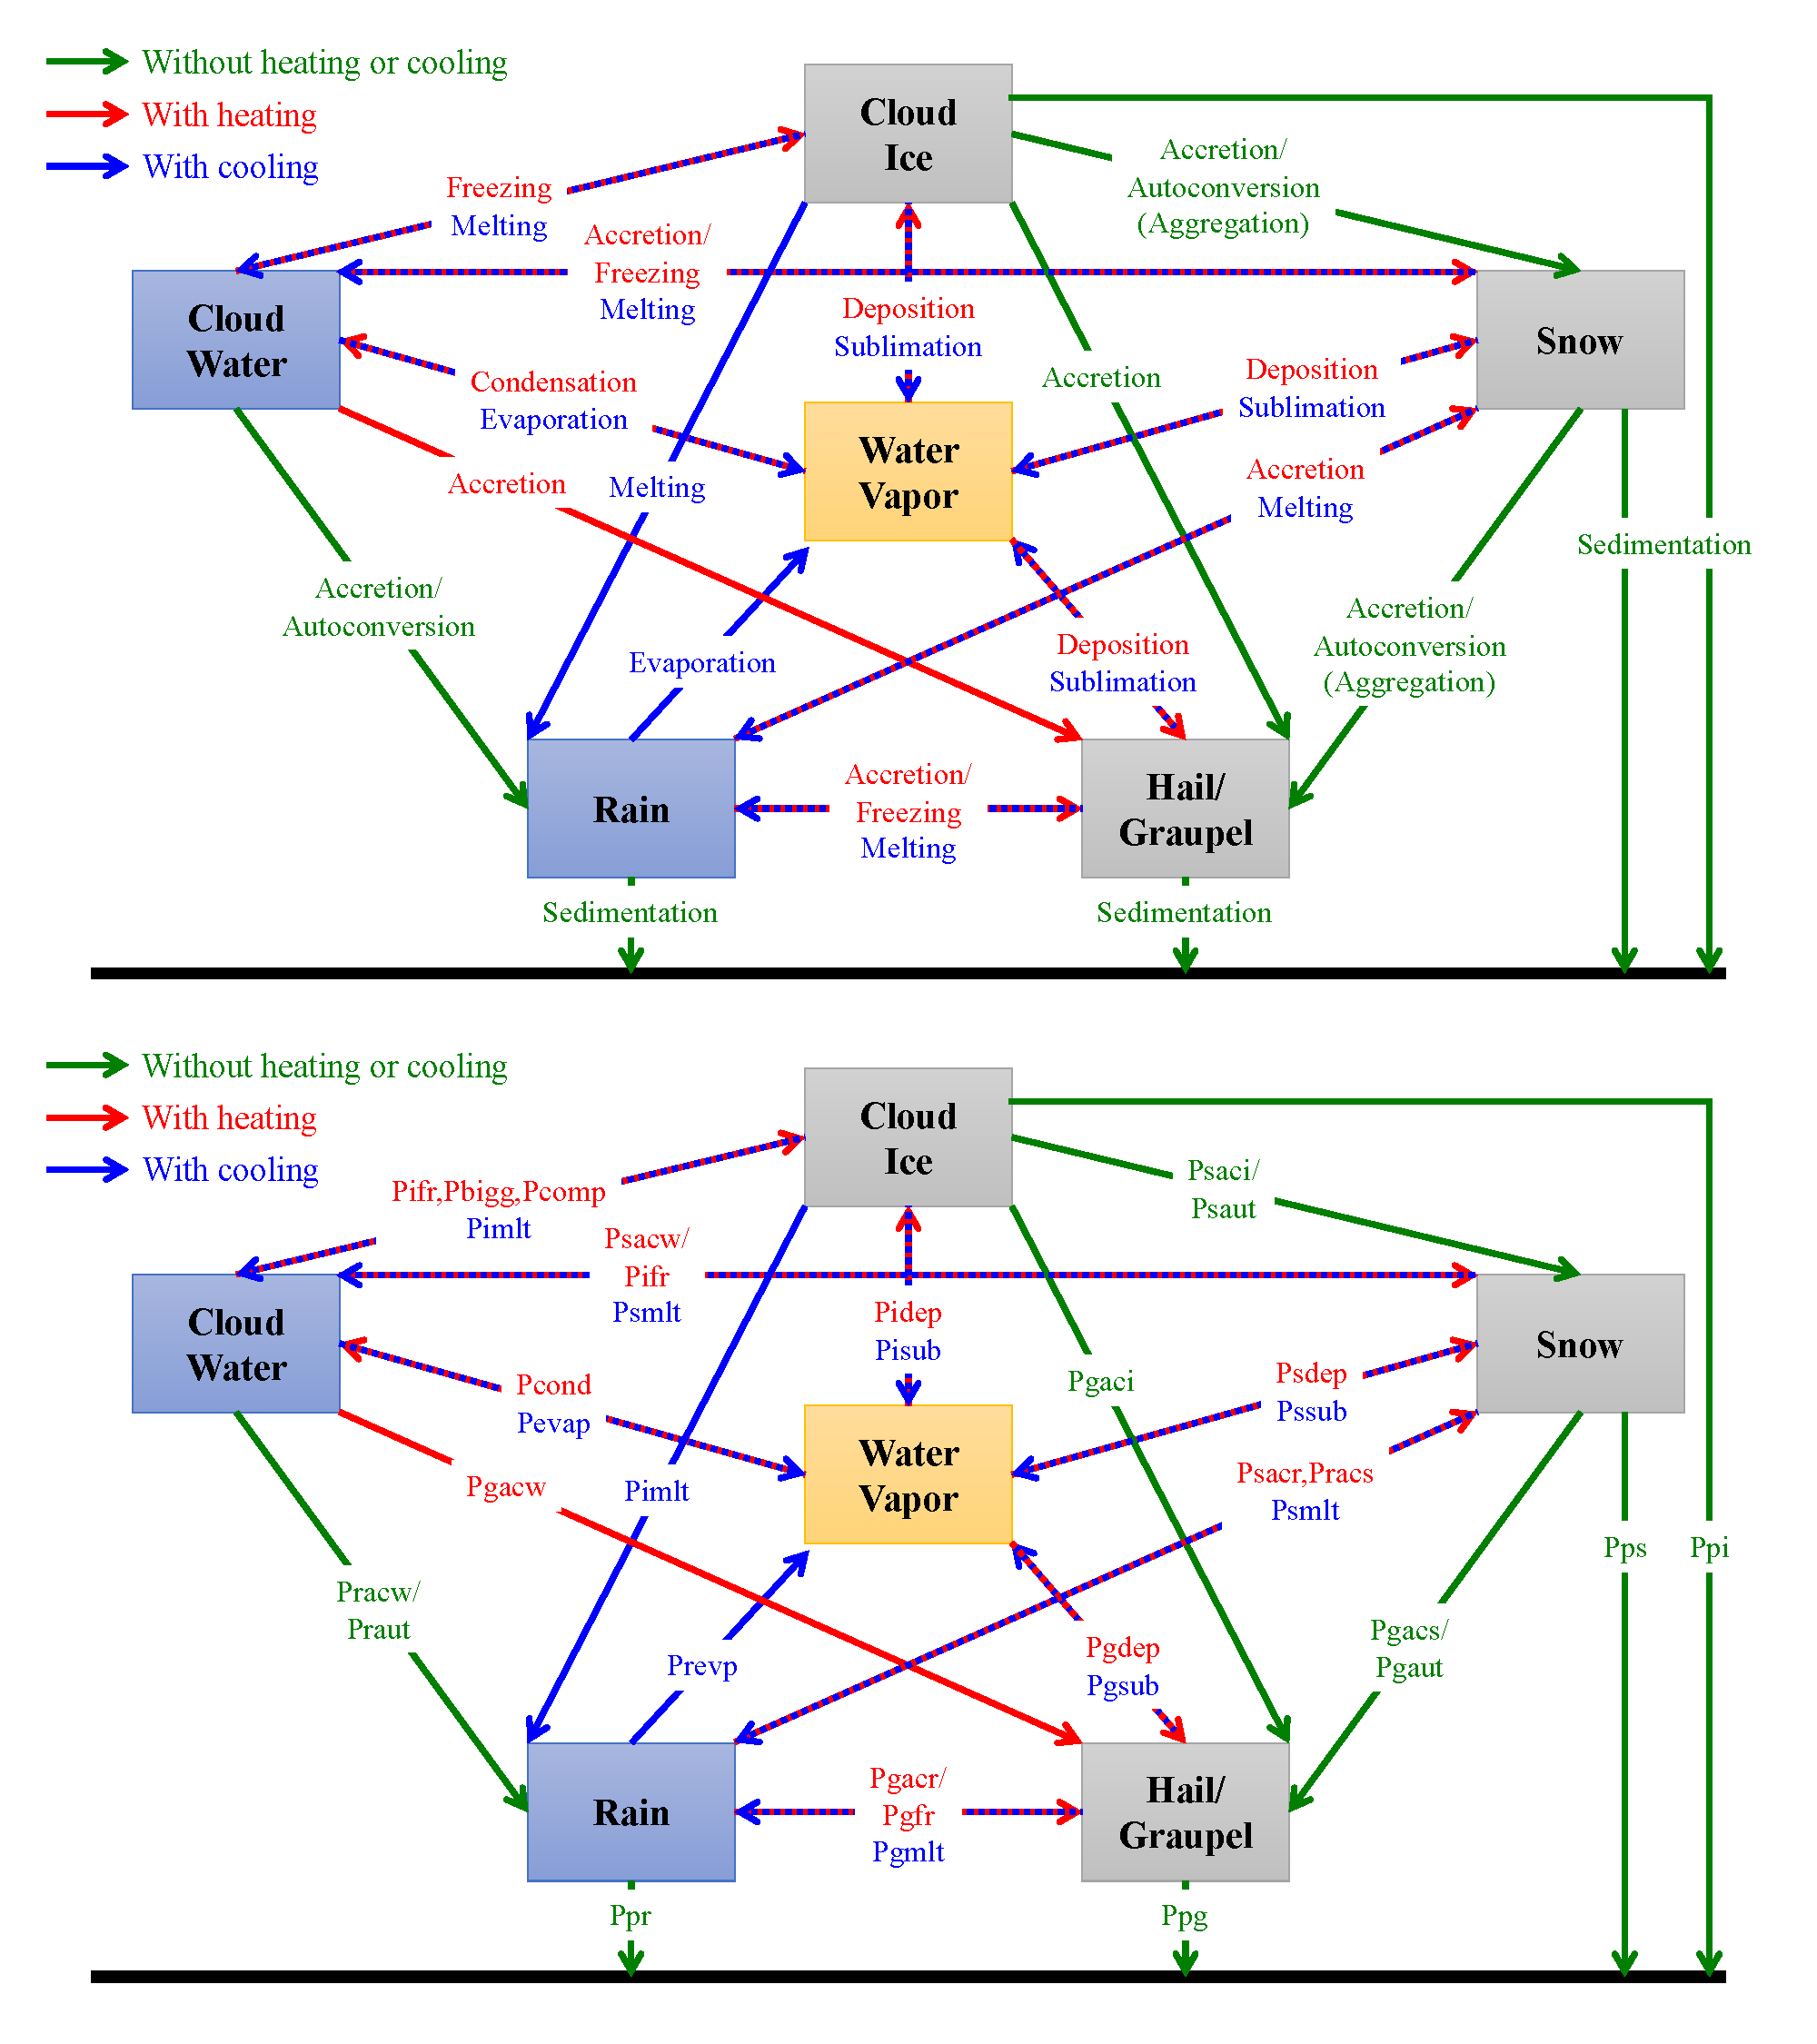
\includegraphics[width=\textwidth]{fig1.pdf}
\caption{Schematic of the GFDL MP. The yellow box indicates prognostic water vapor, blue boxes indicate prognostic liquid-phase hydrometeors, and gray boxes indicate prognostic solid-phase hydrometeors. Red / Blue arrows indicate processes involving heating / cooling from phase changes, while green arrows indicate conversion and sedimentation processes. The bottom panel shows symbols defined in Table \ref{tab:tab1p} and in Equations \eqref{eqn:1:1} to \eqref{eqn:1:13}. This figure is revised from \citet{zhou2019towa}.}
\label{fig:fig1}
\end{figure}

The prognostic equations governing the mass mixing ratio conversion between hydrometeors shown in Figure \ref{fig:fig1} are written as:
\begin{align}
	\dfrac{\partial q_{vapor}}{\partial t} = & Pevap + Pisub + Prevp + Pssub + Pgsub \nonumber \\ & - Pcond - Pidep - Psdep - Pgdep \label{eqn:1:1}\\
	\dfrac{\partial q_{water}}{\partial t} = & Pcond + \alpha Pimlt + \epsilon Psmlt + \epsilon Psacw + \epsilon Psacr + \epsilon Pracs \nonumber \\ & - Pevap - Pifr - Pracw - Praut - Pgacw - Pcomp - Pbigg \\
	\dfrac{\partial q_{ice}}{\partial t} = & Pidep + \beta Pifr + Pcomp + Pbigg \nonumber \\ & - Pisub - Pimlt - Psaci - Psaut - Pgaci \\
	\dfrac{\partial q_{rain}}{\partial t} = & Pracw + Praut + (1 - \alpha) Pimlt + (1 - \epsilon) Psmlt + Pgmlt  + (1 - \epsilon) Pascr \nonumber \\ & + (1 - \epsilon) Pracs + (1 - \epsilon) Psacw + Pgacw + Pgacr \nonumber \\ & - Prevp - Psacr - Pgacr - Pgfr \\
	\dfrac{\partial q_{snow}}{\partial t} = & Psdep + (1 - \beta) Pifr + Psaci + Psaut + Psacr \nonumber \\ & - Pssub - Psmlt - Pracs - Pgacs - Pgaut - Psacw - Psacr \\
	\dfrac{\partial q_{graupel}}{\partial t} = & Pgdep + Pgacw + Pgaci + Pgacr + Pgfr + Pgacs + Pgaut \nonumber \\ & - Pgsub - Pgmlt - Pgacw - Pgacr \label{eqn:1:13},
\end{align}
where $\alpha$, $\beta$, and $\epsilon$ represent the partitioning of $Pimlt$, $Pifr$, $Psmlt$, $Psacw$, $Psacr$, and $Pracs$ in separated microphysical processes. Note that all relevant hydrometeors and temperature are updated immediately after each cloud microphysical process based on exact mass conservation and moist total energy conservation. The meaning and source of each item on the right-hand side of Equations \eqref{eqn:1:1} to \eqref{eqn:1:13} and in Figure \ref{fig:fig1} are demonstrated in Table \ref{tab:tab1p}. Conversion between hydrometeors in different phases involves heating and cooling of the air, while that between hydrometeors in the same phases does not. Most of the microphysical processes, as well as the parameters, are revised from \citet{lin1983bulk, hong2004arev, hong2006thew}.

\begin{table}[!h]
\caption{The symbols used in the prognostic mass mixing ratio equations and Figure \ref{fig:fig1}.}
\label{tab:tab1p}
\begin{tabular}{p{0.1\textwidth}p{0.85\textwidth}}
\hline
Symbol	&	Meaning and Source	\\
\hline
Pcond	&	Condensational growth of cloud water \citep{hong2006thew}.	\\
Pevep	&	Evaporation of cloud water \citep{hong2006thew}.	\\
Pifr	&	Freezing of cloud water to form cloud ice \citep{lin1983bulk, hong2006thew}. Auto-convert to snow if cloud ice exceeds a threshold.	\\
Pbigg	&	Bigg freezing of cloud water to form cloud ice \citep{bigg1953thes}.	\\
Pcomp	&	Complete freezing of cloud water to form cloud ice \citep{lin1983bulk, hong2006thew} \\
Pidep	&	Depositional growth of cloud ice \citep{hong2004arev}.	\\
Pisub	&	Sublimation of cloud ice \citep{hong2004arev}.	\\
Pimlt	&	Melting of cloud ice to form cloud water \citep{lin1983bulk}. Auto-convert to rain if cloud water exceeds a threshold.	\\
Prevp	&	Evaporation of rain \citep{lin1983bulk}.	\\
Praut	&	Auto-conversion of cloud water to form rain \citep{hong2004arev}.	\\
Pracw	&	Accretion of cloud water by rain \citep{lin1983bulk}.	\\
Pracs	&	Accretion of snow by rain; produces graupel if rain or snow exceeds a threshold and $T < T_{freez}$ \citep{lin1983bulk}.	\\
Psacw	&	Accretion of cloud water by snow; produces snow if $T < T_{freez}$ or rain if $T \geq T_{freez}$ \citep{lin1983bulk}.	\\
Psacr	&	Accretion of rain by snow. For $T < T_{freez}$, produces graupel if rain or snow exceeds a threshold; if not, produces snow \citep{lin1983bulk}.	\\
Psaci	&	Accretion of cloud ice by snow \citep{lin1983bulk}.	\\
Psaut	&	Auto-conversion (aggregation) of cloud ice to form snow \citep{lin1983bulk}.	\\
Psdep	&	Depositional growth of snow \citep{lin1983bulk}.	\\
Pssub	&	Sublimation of snow \citep{lin1983bulk}.	\\
Psmlt	&	Melting of snow to form cloud water \citep{lin1983bulk}. Auto-convert to rain if cloud water exceeds a threshold.	\\
Pgaut	&	Auto-conversion (aggregation) of snow to form graupel \citep{lin1983bulk}.	\\
Pgfr	&	Freezing of rain to form graupel \citep{lin1983bulk}.	\\
Pgacw	&	Accretion of cloud water by graupel \citep{lin1983bulk}.	\\
Pgaci	&	Accretion of cloud ice by graupel \citep{lin1983bulk}.	\\
Pgacr	&	Accretion of rain by graupel \citep{lin1983bulk}.	\\
Pgacs	&	Accretion of snow by graupel \citep{lin1983bulk}.	\\
Pgdep	&	Depositional growth of graupel \citep{lin1983bulk}.	\\
Pgsub	&	Sublimation of graupel \citep{lin1983bulk}.	\\
Pgmlt	&	Melting of graupel to form rain, $T \geq T_{freez}$ \citep{lin1983bulk}.	\\
Ppi		&	Sedimentation of cloud ice \citep{deng2008cirr, heymsfield1990asch}.	\\
Ppr		&	Sedimentation of rain \citep{lin1983bulk}.	\\
Pps		&	Sedimentation of snow \citep{lin1983bulk}.	\\
Ppg		&	Sedimentation of graupel \citep{lin1983bulk}.	\\
\hline
\end{tabular}
\end{table}

There are several definitions, assumptions, and conservations that are different from other cloud microphysics schemes. The mass of a grid cell includes that of water vapor and of all hydrometeors; that latent heat coefficients are functions of air temperature; dry air, water vapor, liquid water, and solid water have their own heat capacities; cloud droplet number concentrations are prescribed; subgrid variability is piecewise-linear and scale-aware; saturation water vapor pressure is derived explicitly; latent heating and cooling follow the exact moist total energy conservation. More details will be depicted in this section.

%------------------------------------------------------------------------------

\subsection{Vertical Placement of the Meteorological Fields}

It is important to clarify in advance where the meteorological fields are located in the model vertical levels / layers. Model levels are defined as the boundaries of the model layers. Thus the number of model levels is equal to one more than the number of model layers. Sometimes, model levels are called as interfaces or layer edges. Meteorological fields at model layers in FV3 are always defined as layer-mean values. However, those at model levels are defined as interface (cell face-mean) values.

As it is shown in Figure \ref{fig:fig2}, interface height ($z_{int}$) and interface air pressure ($p_{int}$) are defined at model levels. Zonal wind ($u$), meridional wind ($v$), vertical velocity ($w$), air temperature ($T$), the mass mixing ratio of hydrometeors ($q$), height thickness (negative) ($dz$), pressure thickness or air mass (positive) ($dp$) are defined at model layers. Those are layer-mean variables. We can also get the middle layer height ($z$) and layer-mean air pressure ($p$) using gas law and hydrostatic equilibrium:
\begin{gather}
	p = - \dfrac{dp}{gdz} R_{dry} T_v
\end{gather}
where $T_v$ is virtual temperature, and $R_{dry}$ is dry air constant.

\begin{figure}[h]
\centering
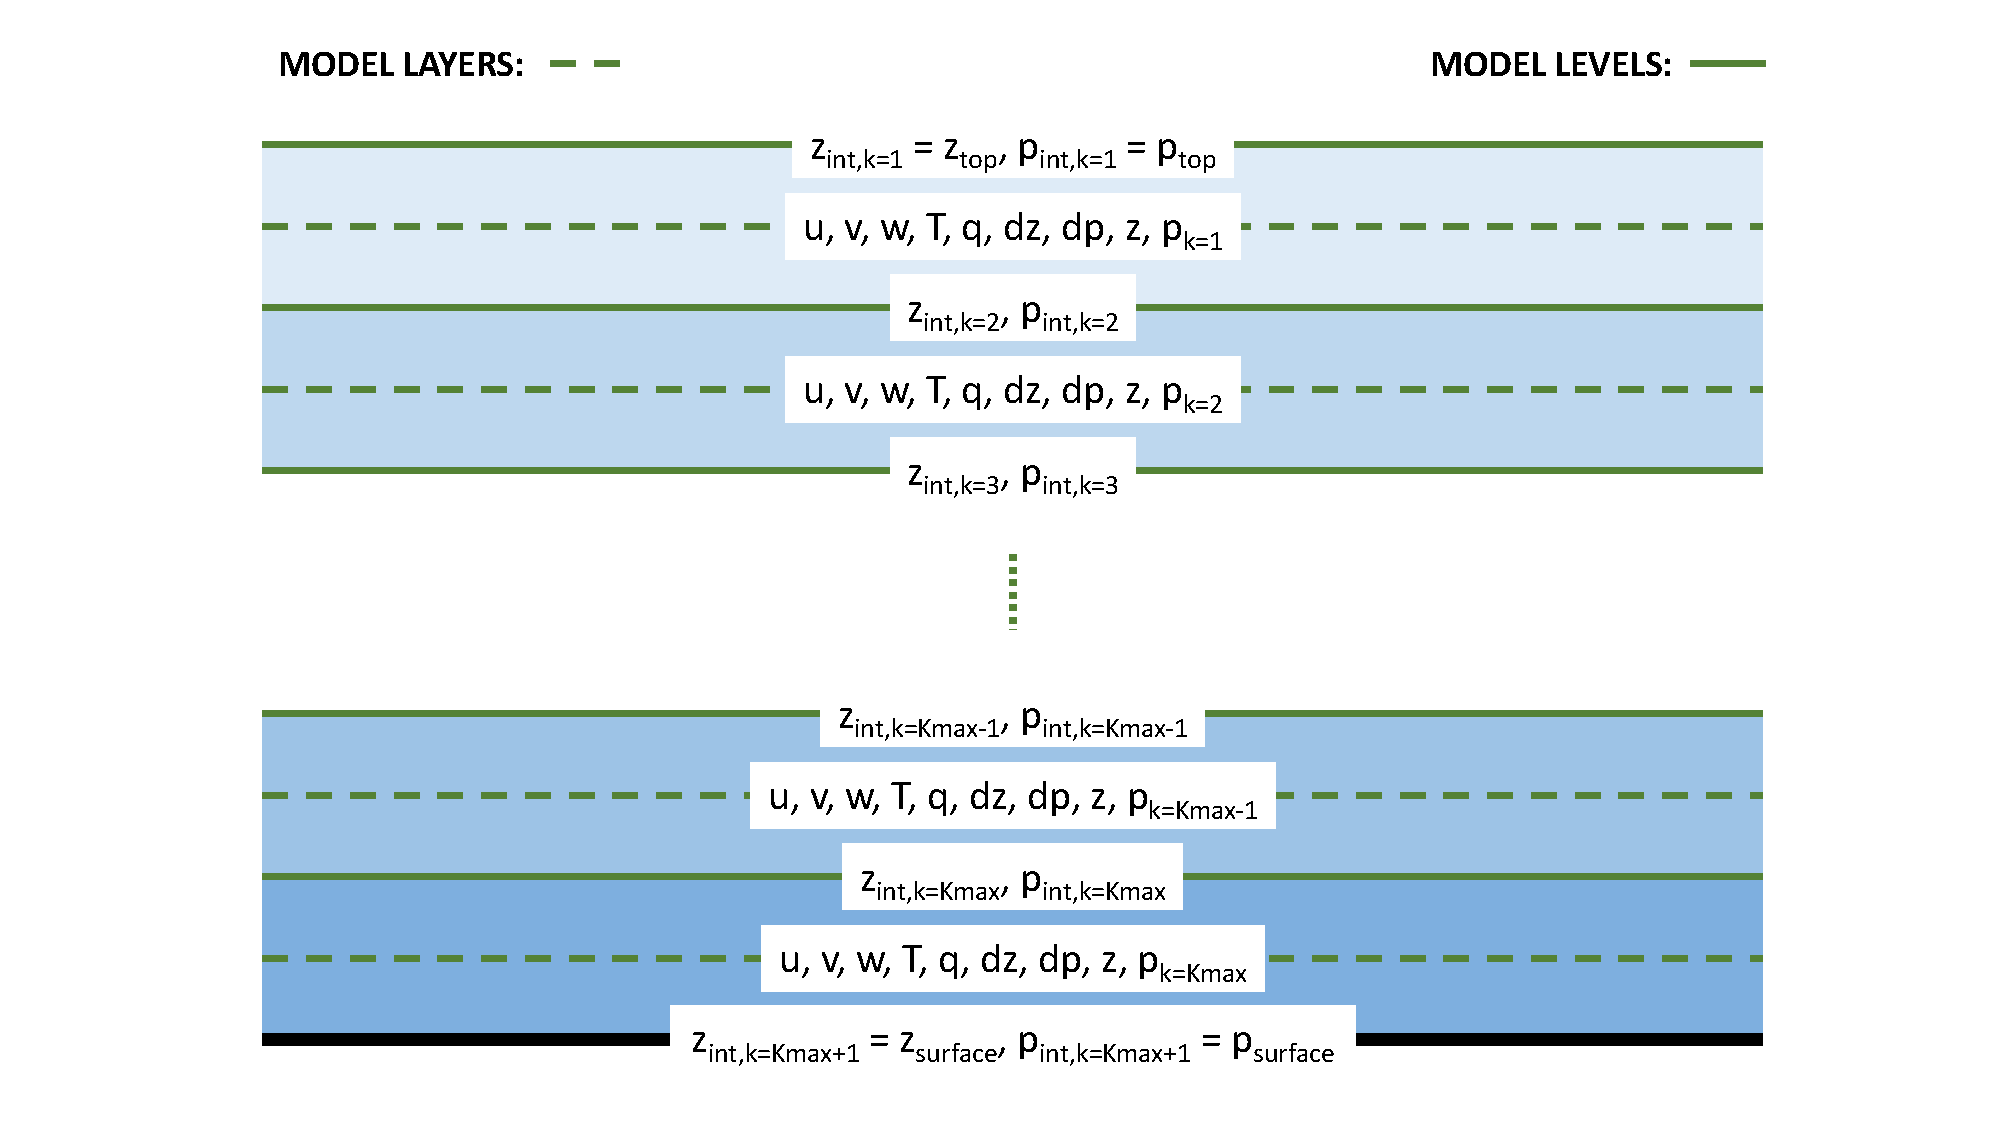
\includegraphics[width=\textwidth]{fig2.pdf}
\caption{Schematic of model layers, model levels, and the location of different meteorological fields.}
\label{fig:fig2}
\end{figure}

%------------------------------------------------------------------------------

\subsection{Size Distribution of Hydrometeors}

The size distribution of hydrometeors is central to a cloud microphysics scheme \citep{khain2018phys}. Many microphysical variables and processes are directly derived from the integration over the size distribution. For example, the mass mixing ratio of hydrometeors is the third moment. The number concentration of hydrometeor is the zeroth moment, the effective radius is the ratio of the third moment and the second moment, and the radar reflectivity is the sixth moment. The terminal velocity and collision are mostly determined by the higher moments of the size distribution. According to observations, the size distribution of non-precipitable hydrometeors (e.g. cloud water and cloud ice) is represented as a gamma distribution, while precipitable hydrometeors (e.g. rain, snow, and graupel) is represented as a exponential distribution \citep{pruppacher2010micr}. The exponential distribution can be treated as a simplified gamma distribution.

However, the size distribution of cloud water and cloud ice in the GFDL MP is assumed to be uniform so far, which is simple but unrealistic. Therefore, the number concentration, effective radius, radar reflectivity, and terminal velocity of cloud water and cloud ice are either prescribed as constant or empirically diagnosed from other variables. The size distribution of rain ($n_{rain}$), snow ($n_{snow}$), and graupel ($n_{graupel}$) is assumed as an exponential distribution and follows \citet{lin1983bulk}:
\begin{gather}
	n_{rain} (D) = n_{rain,0} \exp \left(- \lambda_{rain} D \right) \\
	n_{snow} (D) = n_{snow,0} \exp \left(- \lambda_{snow} D \right) \\
	n_{graupel} (D) = n_{graupel,0} \exp \left(- \lambda_{graupel} D \right)
\end{gather}
where $D$ is the diameter of hydrometeor. $n_{rain,0}$, $n_{snow,0}$, and $n_{graupel,0}$ are the intercept parameters of the rain, snow, and graupel size distributions prescribed as constants. The slope parameters of the rain ($\lambda_{rain}$), snow ($\lambda_{snow}$), and graupel ($\lambda_{graupel}$) size distributions can be derived from the integration of size distribution for all sizes and the mass mixing ratio of hydrometeor:
\begin{gather}
	\lambda_{rain} = \left(\dfrac{\pi \rho_{rain} n_{rain,0}}{\rho q_{rain}} \right)^{0.25} \\
	\lambda_{snow} = \left(\dfrac{\pi \rho_{snow} n_{snow,0}}{\rho q_{snow}} \right)^{0.25} \\
	\lambda_{graupel} = \left(\dfrac{\pi \rho_{graupel} n_{graupel,0}}{\rho q_{graupel}} \right)^{0.25}
\end{gather}
where $\rho_{rain}$, $\rho_{snow}$, and $\rho_{graupel}$ are the density of rain, snow, and graupel. $\rho$ is air density.

%------------------------------------------------------------------------------

\subsection{Air Mass and Mass Mixing Ratio of Hydrometeors}

Air mass per unit area ($M_{dry}$) and the mass mixing ratio of hydrometeors ($q_*$) in the GFDL MP are defined for dry air at the model layers:
\begin{gather}
	M_{dry} = \dfrac{dp}{g} \\
	q_* = \dfrac{M_{*}}{M_{dry}}
\end{gather}
where $dp$ is dry air thickness, $q_*$ can be $q_{vapor}$, $q_{water}$, $q_{ice}$, $q_{rain}$, $q_{snow}$, or $q_{graupel}$, $M_*$ can be $M_{vapor}$, $M_{water}$, $M_{ice}$, $M_{rain}$, $M_{snow}$, or $M_{graupel}$. That is different from those in the FV3 dynamical core, which are defined for moist air (dry air + all hydrometeors) thickness ($dp'$) and the specific ratio of hydrometeors ($q'_*$):
\begin{gather}
	dp' = \left(M_{dry} + M_{vapor} + M_{water} + M_{ice} + M_{rain} + M_{snow} + M_{graupel}\right)g \\
	q'_* = \dfrac{M_{*}}{M_{dry} + M_{vapor} + M_{water} + M_{ice} + M_{rain} + M_{snow} + M_{graupel}}
\end{gather}

At the beginning of the cloud microphysics scheme, moist air thickness ($dp'$) is converted to dry air thickness ($dp$), specific ratio of hydrometeors ($q'_*$) is converted to mass mixing ratio of hydrometeors ($q_*$):
\begin{gather}
	dp = dp' \left[1 - \left(q'_{vapor} + q'_{water} + q'_{ice} + q'_{rain} + q'_{snow} + q'_{graupel} \right) \right] \\
	q_* = \dfrac{q'_*}{1 - \left(q'_{vapor} + q'_{water} + q'_{ice} + q'_{rain} + q'_{snow} + q'_{graupel} \right)}
\end{gather}
At the end of the cloud microphysics scheme, dry air thickness ($dp$) converts back to moist air thickness ($dp'$), mass mixing ratio of hydrometeors ($q_*$) converts back to specific ratio of hydrometeors ($q'_*$):
\begin{gather}
	dp' = dp \left[1 + \left(q_{vapor} + q_{water} + q_{ice} + q_{rain} + q_{snow} + q_{graupel} \right) \right] \\
	q'_* = \dfrac{q_*}{1 + \left(q_{vapor} + q_{water} + q_{ice} + q_{rain} + q_{snow} + q_{graupel} \right)}
\end{gather}
It is important to note that air mass is exactly conserved in the GFDL MP.

%------------------------------------------------------------------------------

\subsection{Number Concentration of Hydrometeors}

In the GFDL MP, the number concentration of hydrometeors are not prognostic variables. For cloud water, the number concentration is only used for cloud water to rain autoconversion and cloud water freezing to form cloud ice. It will be described later that the cloud water number concentration is from the prescribed cloud droplet number concentration, which has constant values over land and over ocean. For cloud ice, the number concentration should be from ice nucleation or cloud ice deposition. For now, it follows the calculation in \citet{hong2004arev}:
\begin{gather}
	N_{ice} = 5.38 \times 10^7 \left(\rho q_{ice} \right)^{0.75}
\end{gather}
Optionally, $N_{ice}$ can also be calculated from \citet{meyers1992newp}:
\begin{gather}
	N_{ice} = \exp \left[-2.80 + 0.262 \times \left(T_{freez} - T \right) \right] \times 1000.0
\end{gather}
or
\begin{gather}
	N_{ice} = \exp \left[-0.639 + 12.96 \times \left(\dfrac{q_{vapor}}{q_{s2}} - 1 \right) \right] \times 1000.0
\end{gather}
$N_{ice}$ can also calculated from \citet{cooper1986icei}:
\begin{gather}
	N_{ice} = 5 \times 10^{-3} \times \exp \left[0.304 \times \left(T_{freez} - T \right) \right] \times 1000.0
\end{gather}
One more option is from \citet{fletcher1962thep}:
\begin{gather}
	N_{ice} = 1 \times 10^{-5} \times \exp \left[0.5 \times \left(T_{freez} - T \right) \right] \times 1000.0
\end{gather}
Since rain, snow, and graupel follow the exponential size distribution, Their number concentrations ($N_{rain}$, $N_{snow}$, and $N_{graupel}$) are the integration of size distributions:
\begin{gather}
	N_{rain} = \int_0^{\infty} n_{rain} (D) dD = \dfrac{n_{rain,0}}{\lambda_{rain}} \\
	N_{snow} = \int_0^{\infty} n_{snow} (D) dD = \dfrac{n_{snow,0}}{\lambda_{snow}} \\
	N_{graupel} = \int_0^{\infty} n_{graupel} (D) dD = \dfrac{n_{graupel,0}}{\lambda_{graupel}}
\end{gather}
If, in the future, number concentration is a prognostic variable in this cloud microphysics scheme, $n_{rain,0}$, $n_{snow,0}$, and $n_{graupel,0}$ will no longer be constants. Instead, they are updated upon the change of mass mixing ratio and number concentration written as:
\begin{gather}
	n_{rain,0} = \left(\dfrac{\pi \rho_{rain}}{\rho q_{rain}} \right)^{1/3} N_{rain}^{4/3} \\
	n_{snow,0} = \left(\dfrac{\pi \rho_{snow}}{\rho q_{snow}} \right)^{1/3} N_{snow}^{4/3} \\
	n_{graupel,0} = \left(\dfrac{\pi \rho_{graupel}}{\rho q_{graupel}} \right)^{1/3} N_{graupel}^{4/3}
\end{gather}

%------------------------------------------------------------------------------

\subsection{Air Density}

Many assumptions in the GFDL MP depend on whether the model, particularly the FV3 dynamical core, is designed to be hydrostatic or non-hydrostatic. For climate modeling, the hydrostatic assumption is appropriate. In this case, the GFDL MP uses the consistent definition of constants and parameters as other physical parameterizations. As the resolutions approach the grey zone, the hydrostatic assumption is no longer as accurate and it is more appropriate to use non-hydrostatic dynamics. In either case, energy conservation and the consistency of constants and parameterizations are critical. 

In hydrostatic case, moist air thickness ($dp'$) and air temperature ($T$) are both prognostic variables in the dynamical core. So air density ($\rho$) is calculated using the ideal gas law and the hypsometric equation:
\begin{gather}
	\rho = \dfrac{p}{R_{dry} T_v} = \dfrac{dp'}{d \ln p' R_{dry} T_v}
\end{gather}
where $T_v$ is virtual temperature, $R_{dry}$ is dry air gas constant.

In non-hydrostatic case, the height thickness (negative) ($dz$) is also a prognostic variable. So air density ($\rho$) is calculated from its definition:
\begin{gather}
	\rho = - \dfrac{dp'}{g dz}
\end{gather}
where $g$ is gravitational acceleration.

%------------------------------------------------------------------------------

\subsection{Virtual Temperature}

The virtual temperature ($T_{v}$) of a moist air parcel is the temperature at which a theoretical dry air parcel would have a total pressure and density equal to the moist parcel of air. Thus all hydrometeors are considered to calculate virtual temperature:
\begin{equation}
	T_v = T \left(1 + z_{vir} q_{vapor} \right) \left[1 - \left(q_{vapor} + q_{water} + q_{ice} + q_{rain} + q_{snow} + q_{graupel} \right) \right] \footnote{This differs slightly from the IFS formula: $T_v = T \left[1 + z_{vir} q_{vapor} - \left(q_{vapor} + q_{water} + q_{ice} + q_{rain} + q_{snow} + q_{graupel} \right) \right]$ (\url{https://www.ecmwf.int/en/elibrary/18714-part-iv-physical-processes} Chapter 12. The difference is of order $q_{vapor}q_{*} \ll q_{*}$ while reducing the number of computations within the code.)}
\end{equation}
where $z_{vir}$ is the ratio of the gas constants of water vapor ($R_{vapor}$) and dry air ($R_{dry}$):
\begin{gather}
	z_{vir} = \dfrac{R_{vapor}}{R_{dry}} - 1
\end{gather}

%------------------------------------------------------------------------------

\subsection{Specific Heat Capacity}

In the real atmosphere, the air contains water vapor and hydrometeors. Thus, the specific heat capacity consists of contributions from both dry air, water vapor, and each hydrometeor. In the GFDL MP, the constant-volume or constant-pressure specific heat capacity for moist air ($c_{v,moist}$ or $c_{p,moist}$) is defined as:
\begin{gather}
	c_{v,moist} = c_{v,dry} + q_{vapor} c_{v,vapor} + q_{liquid} c_{v,liquid} + q_{solid} c_{v,solid} \\
	c_{p,moist} = c_{p,dry} + q_{vapor} c_{p,vapor} + q_{liquid} c_{p,liquid} + q_{solid} c_{p,solid}
\end{gather}
where $c_{v,dry}$, $c_{v,vapor}$, $c_{v,liquid}$, and $c_{v,solid}$ are the constant-volume specific heat capacities of dry air, water vapor, liquid water (at the triple point of water $T_{freez}$), and solid water (at the triple point of water $T_{freez}$). Similarly, $c_{p,dry}$, $c_{p,vapor}$, $c_{p,liquid}$, and $c_{p,solid}$ are the corresponding specific heat capacities at constant pressure. Liquid water and solid water barely change in volume and pressure during heating or cooling that their constant-volume and constant-pressure specific heat capacities are the same and defined as:
\begin{gather}
	c_{liquid} = c_{v,liquid} = c_{p,liquid} \\
	c_{solid} = c_{v,solid} = c_{p,solid}
\end{gather}
$q_{liquid}$ is the mass mixing ratio of liquid water defined as the sum of the mass mixing ratio of cloud water and rain:
\begin{gather}
	q_{liquid} = q_{water} + q_{rain}
\end{gather}
and $q_{solid}$ is the mass mixing ratio of solid water defined as the sum of mass mixing ratio of cloud ice, snow, and graupel:
\begin{gather}
	q_{solid} = q_{ice} + q_{snow} + q_{graupel}
\end{gather}
The sum of the mass mixing ratio of liquid and solid water ($q_{cond}$) is written as:
\begin{gather}
	q_{cond} = q_{liquid} + q_{solid}
\end{gather}

Different from most existing cloud microphysics schemes, the GFDL MP was built at the height coordinate. That means heating or cooling in this cloud microphysics scheme uses the constant-volume specific heat capacity. Pressure thickness is later adjusted according to the change of hydrometeors content in the grid box. This treatment is consistent with what is being used in FV3's nonhydrostatic solver \citep{lin2004aver}, and the Nonhydrostatic ICosahedral Atmospheric Model (NICAM) \citep{satoh2008nonh}. Theoretically and actually, the constant-pressure specific heat capacity is about $40\%$ larger than the constant-volume specific heat capacity. It indicates the heating or cooling by using constant-pressure specific heat capacity is $40\%$ smaller than that using constant-volume specific heat capacity. Since the height thickness will be later adjusted according to temperature change, the eventual impact of the microphysics processes on the atmosphere is similar in these two different approaches. In the following sections, we use $c_{moist}$ instead of $c_{v,moist}$ as default.

%------------------------------------------------------------------------------

\subsection{Latent Heat Coefficient}

According to the Kirchhoff's equation under constant volume \citep{emanuel1994atmo}, the latent heat coefficient of condensation / evaporation ($L_{v2l}$), melting / freezing ($L_{l2s}$), and deposition / sublimation ($L_{v2s}$) are a function of temperature ($T$):
\begin{gather}
	L_{v2l} = L_{vap} + \left(c_{vapor} - c_{liquid} \right) \left( T - T_{freez} \right) \\
	L_{l2s} = L_{fus} + \left(c_{liquid} - c_{solid} \right) \left( T - T_{freez} \right) \\
	L_{v2s} = L_{vap} + L_{fus} + \left(c_{vapor} - c_{solid} \right) \left( T - T_{freez} \right)
\end{gather}
where $L_{vap}$ and $L_{fus}$ are the latent heat coefficient of condensation / evaporation and melting / freezing at the triple point temperature of water ($T_{freez}$). $c_{vapor} = c_{p,vapor}$ in hydrostatic case. $c_{vapor} = c_{v,vapor}$ in non-hydrostatic case.

A special latent heat coefficient of condensation / evaporation ($L'_{v2l}$) for saturated water vapor is defined as:
\begin{gather}
	L'_{v2l} = L_{v2l} + L_{l2s} \max \left[0, \min \left(1, \dfrac{T_{freez} - T}{T_{freez} - T_{wfr}} \right) \right]
\end{gather}
If temperature is higher than freezing temperature ($T > T_{freez}$), $L'_{v2l} = L_{v2l}$; If temperature is lower than critical freezing temperature ($T < T_{wfr}$), $L'_{v2l} = L_{v2s}$; otherwise ($T_{wfr}< T < T_{freez}$), $L_{v2l}< L'_{v2l} < L_{v2s}$.  

%------------------------------------------------------------------------------

\subsection{Cloud Condensation Nuclei and Cloud Droplet Number Concentration}

Cloud condensation nuclei (CCN) is used in cloud seeding, that tries to promote condensation into cloud water by seeding the air with condensation nuclei. It is a major source of cloud water formation. The cloud droplet number concentration (CDNC) activated from CCN determines how much cloud water can be auto-converted to rain. However, since there is no cloud water activation built in this cloud microphysics scheme, the cloud droplet number concentration (CDNC, $N_c$) is either prescribed over land ($N_{c,land}$) and ocean ($N_{c,ocean}$) respectively:
\begin{gather}
    N_c = \left[N_{c,land} \cdot LSM + N_{c,ocean} \cdot \left(1 - LSM \right) \right] \times 10^6
\end{gather}
or calculated from aerosol mass mixing ratio ($q_{aerosol}$) following \citet{boucher1995thes}:
\begin{gather}
    N_c = \left[10^{2.24} \times \left(10^9 \rho q_{aerosol} \right)^{0.257} \cdot LSM + 10^{2.06} \times \left(10^9 \rho q_{aerosol} \right)^{0.48} \cdot \left(1 - LSM \right) \right] \times 10^{6}
\end{gather}
where $LSM$ is the land-sea mask, with value 1 over land and value 0 over ocean. $\rho_{bot}$ is the bottom layer air density. The former method is used in the current operational GFS, NASA GEOS-5, HiRAM, IAP climate model. The latter method is an option in the GFDL modeling system suites. The number concentration of cloud then from the cloud droplet number concentration (CDNC):
\begin{gather}
	N_{water} = N_c
\end{gather}

%------------------------------------------------------------------------------

\subsection{Subgrid Variability}

In a model that is unable to resolve cloud microphysical processes explicitly, it is useful to prescribe the subgrid distribution of quantities (e.g., hydrometeors) in the grid box. Regardless of which algorithm is used, it is some kind of empirical assumption. The simplest one is a linear assumption. In the GFDL MP, it presumed a linear background horizontal variability ($h_{var}$) and vertical variability ($z_{var}$) for hydrometeors following \citet{lin1994acla}.

The horizontal subgrid variability is a function of cell area:
\begin{gather}
	h_{var} = \min \left(0.2, \max \left\{0.01, \left[D_{land} \cdot LSM + D_{ocean} \cdot \left(1 - LSM \right) \right] \sqrt{\dfrac{x}{10^5}} \right\} \right)
\end{gather}
where $x$ is grid size. $D_{land}$ and $D_{ocean}$ are basic value for subgrid variability over land and ocean. These are tunable parameters. This formula indicates larger subgrid variability appears in the larger cell area. $D_{land}$ and $D_{ocean}$ can adjust the strength of the subgrid variability. The subgrid variability function enables the GFDL MP to be flexibly adapted to simulations in different resolutions and variable resolution. Theoretically, this assumption can be applied to all condensation / evaporation, freezing / melting, and deposition / sublimation processes. In the current version of GFDL MP, horizontal subgrid variability is mainly used in the calculation of cloud water to rain autoconversion and cloud fraction diagnostic.

The vertical subgrid variability depends on the distribution of the three adjacent mass mixing ratio of hydrometeors: for model top ($k = 1$) and bottom layer ($k = kbot$):
\begin{gather}
	z_{var,1} = 0 \\
	z_{var,kbot} = 0
\end{gather}
for all other model layers ($k = 2, kbot - 1$), use twice the strength of the positive definiteness limiter \citep{lin1994acla}. Four conditions are considered shown in Figure \ref{fig:fig3}:

\begin{figure}[h]
\centering
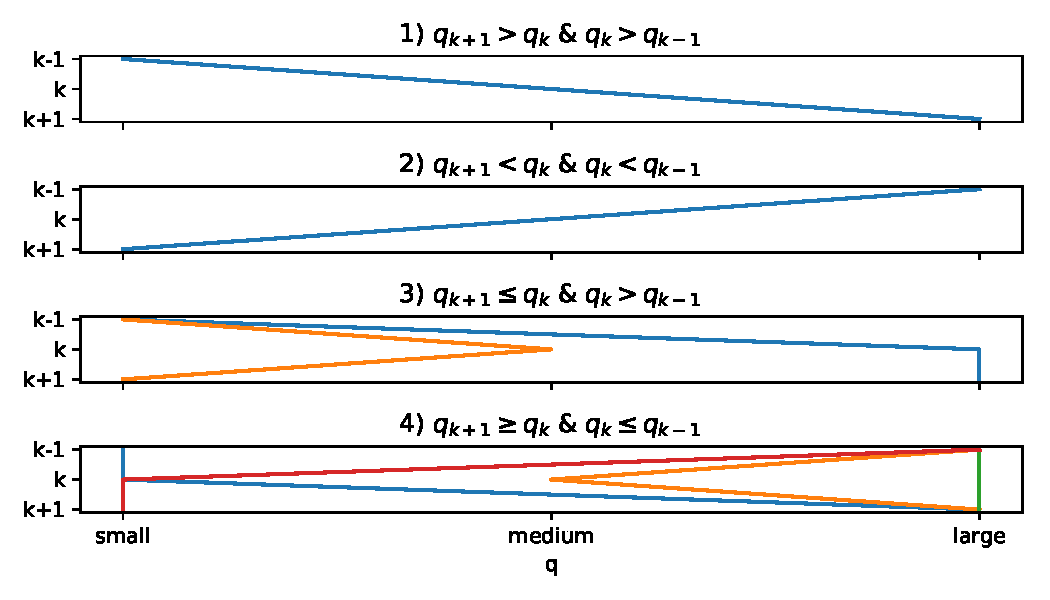
\includegraphics[width=\textwidth]{fig3.pdf}
\caption{Four different conditions of hydrometeor vertical profile in the adjacent three layers. Blue, orange, and red vertical profiles are three different possibles in each condition.}
\label{fig:fig3}
\end{figure}

1) When $q_{k+1} > q_{k}$, and $q_{k} > q_{k-1}$, monotonically increasing from up to down:
\begin{gather}
	z_{var,k} = \dfrac{1}{2} \min \left(\left|\dfrac{q_{k+1} - q_{k-1}}{2} \right|, \dfrac{q_{k}}{2} \right)
\end{gather}
2) When $q_{k+1} < q_{k}$, and $q_{k} < q_{k-1}$, monotonically decreasing from up to down:
\begin{gather}
	z_{var,k} = \dfrac{1}{2} \min \left(\left|\dfrac{q_{k+1} - q_{k-1}}{2} \right|, \dfrac{q_{k}}{2} \right)
\end{gather}
3) When $q_{k+1} \leq q_{k}$, and $q_{k} > q_{k-1}$, maximum value at the center:
\begin{gather}
	z_{var,k} = \min \left[\dfrac{1}{2} \min \left(\left|\dfrac{q_{k+1} - q_{k-1}}{2} \right|, \dfrac{q_{k}}{2} \right), \dfrac{q_{k} - q_{k-1}}{2}, - \dfrac{q_{k+1} - q_{k}}{2} \right]
\end{gather}
4) When $q_{k+1} \geq q_{k}$, and $q_{k} \leq q_{k-1}$, minimum value at the center:
\begin{gather}
	z_{var,k} = 0.0
\end{gather}

Impose a presumed background horizontal variability that is proportional to the value itself:
\begin{gather}
	z_{var,k} = \max \left(z_{var,k}, q_{minvapor}, h_{var} q_k \right), \quad k = 1,...,kbot
\end{gather}

Note that $z_{var}$ is a function of $q$, so $z_{var}$ is different in each hydrometeor. $q_{minvapor}$ is minimum value for water vapor. Vertical subgrid variability is mainly used in the calculation of cloud water to rain autoconversion.

%------------------------------------------------------------------------------

\subsection{Rate of Conversion}

In general, conversion between two hydrometeors is not done instantaneously except for some extreme conditions. In most cases, it is a function of time. If the cloud microphysics scheme is embedded in the FV3 dynamical core, it will use the vertical remapping time step ($dt_m$), which is a sub-cycle of physics time step ($dt_p$) controlled by \textit{k\_split} in the namelists. If the cloud microphysics scheme is inside the normal physics package, it uses a relative smaller cloud microphysics time step ($dt_c$), which is also a sub-cycle of physics time step ($dt_p$). $dt_p$, $dt_m$, $dt_c$ at this stage are the same. However, $dt_p$, $dt_m$ and $dt_c$ have much freedom to control separately, especially for higher resolution.

In many microphysical processes of this cloud microphysics scheme, the effective conversion rate from $x$ to $y$ over a time step $dt$, assuming an exponential decrease of $x$, is calculated as:
\begin{gather}
	f_{x2y} = 1 - \exp \left(-\dfrac{dt}{\tau_{x2y}} \right)
\end{gather}
where $x$ and $y$ can be $v$ (water vapor), $w$ (cloud water), $i$ (cloud ice), $r$ (rain), $s$ (snow), or $g$ (graupel). $dt$ can be $dt_{m}$ or $dt_{c}$. Note that $\tau_{x2y}$ and $\alpha$ are both tunable parameters controlling the conversion rate. The larger of $\tau_{x2y}$, the slower the conversion. 

%------------------------------------------------------------------------------

\subsection{Fix Negative Hydrometeors}

Unphysical negative hydrometeor concentrations are difficult to completely avoid in finite-precision arithmetic. Fixing negative hydrometeors in the GFDL MP is straightforward and mass conserved. The easiest way to fix negative hydrometeor is to borrow mass from other hydrometeors. Negative hydrometeor then is fixed to zero. Assume hydrometeor $x$ is negative, and borrow mass from hydrometeor $y$:
\begin{gather} \label{eq:negfix}
	q_y = q_y + q_x \\
	q_x = 0.0
\end{gather}
In some certain conditions, $q_y$ could become negative after this process. Then $q_y$ need to be fixed from other hydrometeors except for $q_x$. In general, the direction of negative fixing follows:
\begin{gather}
	q_{ice} \leftarrow q_{snow} \leftarrow q_{graupel} \leftarrow q_{rain} \leftarrow q_{water} \leftarrow q_{vapor}
\end{gather}
That is to say, if $q_{ice}$ is negative, borrow mass from $q_{snow}$; if $q_{snow}$ is negative, borrow mass from $q_{graupel}$; etc. However, to prevent overdoing, Equation (\ref{eq:negfix}) can be revised as:
\begin{gather}
	q_{tmp} = \min \left[ - q_x, \max \left(0, q_y \right) \right] \\
	q_x = q_x + q_{tmp} \\
	q_y = q_y - q_{tmp}
\end{gather}
If this is a phase change, latent heating and cooling should also be applied.

In the GFDL MP, water vapor can be used to fix all other negative hydrometeors. However, when water vapor is negative, it can borrow from above and below layers. From $k = 1$ to $kbot - 1$, when water vapor at $k$ layer is negative, borrow it from below:
\begin{gather}
	q_{vapor,k+1} = q_{vapor,k+1} + \dfrac{q_{vapor,k} dp_k}{dp_{k+1}} \\
	q_{vapor,k} = 0
\end{gather}
when water vapor at the bottom layer is negative, borrow it from above if the water vapor in $kbot - 1$ is positive:
\begin{gather}
	dq = \min \left[-q_{vapor,kbot} dp_{kbot}, q_{vapor,kbot-1} dp_{kbot-1} \right] \\
	q_{vapor,kbot-1} = q_{vapor,kbot-1} - \dfrac{dq}{dp_{kbot-1}} \\
	q_{vapor,kbot} = q_{vapor,kbot} + \dfrac{dq}{dp_{kbot}}
\end{gather}

%------------------------------------------------------------------------------

\subsection{Saturation Water Vapor Pressure}

Saturation water vapor pressure is calculated using lookup tables. Five lookup tables are designed for different purposes for the GFDL MP. First of all, define a scaled temperature
\begin{gather}
	T'^* = \min \left\{2621, 10 \left[T - \left(T_{freez} - 160 \right) \right] + 1 \right\} \\
	T^* = \textrm{INT} \left(T'^* \right)
\end{gather}
$\textrm{INT}$ here means forcing a variable to be an integer. Different from most existing tables of saturation water vapor pressure, which are basically written as empirical formula, the ones in the GFDL MP are directly derived by integrating of the Clausius-Claperyron equation \citep{wallace1977atmo}:
\begin{gather}
	\dfrac{d \ln e_{s*}}{dT} = \dfrac{L_*}{R_{vapor} T^2}
\end{gather}
where $e_{s*}$ can be $e_s0$, $e_{s1}$, or $e_{s2}$ detailedly described in the following sub-sections. $L_*$ can be $L_{v2l}$, $L_{l2s}$, or $L_{v2s}$.

%------------------------------------------------------------------------------

\subsubsection*{Table N}

The table N of saturation water vapor pressure ($e_{s0}$) was built only over water with temperature ranged from $-160^\circ C$ to $102^\circ C$ defined as:
\begin{gather}
	T_{tmp} = T_{freez} - 160 + 0.1\left( T^* - 1 \right) \\
	\alpha = {\dfrac{\left(c_{p,vapor} - c_{liquid} \right) \ln \dfrac{T_{tmp}}{T_{freez}} + \left[L_{vap} - T_{freez} \left(c_{p,vapor} - c_{liquid} \right) \right] \dfrac{T_{tmp} - T_{freez}}{T_{tmp} T_{freez}}}{R_{vapor}}} \\
	e_{s0}(T^*) = e_0 e^{\alpha}
\end{gather}

%------------------------------------------------------------------------------

\subsubsection*{Table I}

The table I of saturation water vapor pressure ($e_{s1}$) was built based on three temperature categories:

1) When $T^*$ ranges from 1 to 1600 ($T$ ranges from $-160^\circ C$ to $0^\circ C$), compute saturation water vapor pressure ($e_{s1}$) over ice:
\begin{gather}
	T_{tmp} = T_{freez} - 160 + 0.1\left( T^* - 1 \right) \\
	\alpha = {\dfrac{\left(c_{p,vapor} - c_{solid} \right) \ln \dfrac{T_{tmp}}{T_{freez}} + \left[L_{vap} + L_{fus} - T_{freez} \left(c_{p,vapor} - c_{solid} \right) \right] \dfrac{T_{tmp} - T_{freez}}{T_{tmp} T_{freez}}}{R_{vapor}}} \\
	e_{s1}(T^*) = e_0 e^{\alpha}
\end{gather}
where $e_0$ is saturation vapor pressure at $T_{freez}$.

2) When $T^*$ ranges from 1401 to 2621 ($T$ ranges from $-20^\circ C$ to $102^\circ C$), compute saturation water vapor pressure ($e_{s1}$) over water:
\begin{gather}
	T_{tmp} = T_{freez} - 20 + 0.1\left( T^* - 1400 - 1 \right) \\
	\alpha = {\dfrac{\left(c_{p,vapor} - c_{liquid} \right) \ln \dfrac{T_{tmp}}{T_{freez}} + \left[L_{vap} - T_{freez} \left(c_{p,vapor} - c_{liquid} \right) \right] \dfrac{T_{tmp} - T_{freez}}{T_{tmp} T_{freez}}}{R_{vapor}}} \\
	e_{s1}(T^*) = e_0 e^{\alpha}
\end{gather}

3) When $T^*$ ranges from 1401 to 1600 ($T$ ranges from $-20^\circ C$ to $0^\circ C$), compute saturation water vapor pressure ($e_{s1}$) over ice and supercooled water:
\begin{gather}
	T_{tmp} = T_{freez} - 20 + 0.1\left( T^* - 1400 - 1 \right) \\
	e_{s1}(T^*) = \dfrac{\left(T_{freez} - T_{tmp} \right)}{20} e_{s1}(T^*) + \dfrac{\left[T_{tmp} - \left(T_{freez} - 20 \right) \right]}{20} e_{s1}(T^*)
\end{gather}

Note that the first $e_{s1}(T^*)$ on the right hand side comes from saturation water vapor pressure over ice between $-160^\circ C$ and $0^\circ C$, and the second $e_{s1}(T^*)$ on the right hand side comes from saturation water vapor pressure over water between $-20^\circ C$ and $102^\circ C$.

%------------------------------------------------------------------------------

\subsubsection*{Table II}

The table II of saturation water vapor pressure ($e_{s2}$) was built based on two categories:

1) When $T^*$ ranges from 1 to 1600 ($T$ ranges from $-160^\circ C$ to $0^\circ C$), compute saturation water vapor pressure ($e_{s2}$) over ice:
\begin{gather}
	T_{tmp} = T_{freez} - 160 + 0.1\left( T^* - 1 \right) \\
	\alpha = {\dfrac{\left(c_{p,vapor} - c_{solid} \right) \ln \dfrac{T_{tmp}}{T_{freez}} + \left[L_{vap} + L_{fus} - T_{freez} \left(c_{p,vapor} - c_{solid} \right) \right] \dfrac{T_{tmp} - T_{freez}}{T_{tmp} T_{freez}}}{R_{vapor}}} \\
	e_{s2}(T^*) = e_0 e^{\alpha}
\end{gather}

2) When $T^*$ ranges from 1601 to 2621 ($T$ ranges from $0^\circ C$ to $102^\circ C$), compute saturation water vapor pressure ($e_{s2}$) over water:
\begin{gather}
	T_{tmp} = T_{freez} - 160 + 0.1\left( T^* - 1 \right) \\
	\alpha = {\dfrac{\left(c_{p,vapor} - c_{liquid} \right) \ln \dfrac{T_{tmp}}{T_{freez}} + \left[L_{vap} - T_{freez} \left(c_{p,vapor} - c_{liquid} \right) \right] \dfrac{T_{tmp} - T_{freez}}{T_{tmp} T_{freez}}}{R_{vapor}}} \\
	e_{s2}(T^*) = e_0 e^{\alpha}
\end{gather}

A smoother was added to $e_{s2}$ where temperature is around $0^\circ C$ ($T^* = 1600$ and $T^* = 1601$):
\begin{gather}
	e_{s2}(T^*) = 0.25 e_{s2}(T^*-1) + 2 e_s(T^*) + e_{s2}(T^*+1)
\end{gather}

%------------------------------------------------------------------------------

\subsubsection*{Table III}

The table III of saturation water vapor pressure ($e_{s3}$) is the same as Table I except using the Smithsonian formula \citet{smithsonian1951smith}:

1) When $T^*$ ranges from 1 to 1600 ($T$ ranges from $-160^\circ C$ to $0^\circ C$), compute saturation water vapor pressure ($e_{s3}$) over ice:
\begin{gather}
	T_{tmp} = T_{freez} - 160 + 0.1\left( T^* - 1 \right) \\
	a = - 9.09718 \times \left(\dfrac{T_{freez}}{T_{tmp}} - 1 \right) \\
	b = - 3.56654 \times \log_{10} \left(\dfrac{T_{freez}}{T_{tmp}} \right) \\
	c = - 0.876793 \times \left(\dfrac{T_{tmp}}{T_{freez}} - 1 \right) \\
	e = \log_{10} \left(6107.1 \right) \\
	e_{s3}(T^*) = 0.1 \times 10^{a + b + c + d}
\end{gather}

2) When $T^*$ ranges from 1401 to 2621 ($T$ ranges from $-20^\circ C$ to $102^\circ C$), compute saturation water vapor pressure ($e_{s3}$) over water:
\begin{gather}
	T_{tmp} = T_{freez} - 20 + 0.1\left( T^* - 1400 - 1 \right) \\
	a = - 7.90298 \times \left(\dfrac{T_{freez} + 100}{T_{tmp}} - 1. \right) \\
	b = 5.02808 \times \log_{10} \left(\dfrac{T_{freez} + 100}{T_{tmp}} \right) \\
	c = - 1.3816 \times 10^{-7} \times \left[10^{11.344 \times \left(1 - \dfrac{T_{tmp}}{T_{freez} + 100} \right)} - 1 \right] \\
	d = 8.1328 \times 10^{-3} \times \left[10^{3.49149 \times \left(1 - \dfrac{T_{freez} + 100}{T_{tmp}} \right)} - 1. \right] \\
	e = \log_{10} \left(1013246.0 \right) \\
	e_{s3}(T^*) = 0.1 \times 10^{a + b + c + d}
\end{gather}

3) When $T^*$ ranges from 1401 to 1600 ($T$ ranges from $-20^\circ C$ to $0^\circ C$), compute saturation water vapor pressure ($e_{s3}$) over ice and supercooled water:
\begin{gather}
	T_{tmp} = T_{freez} - 20 + 0.1\left( T^* - 1400 - 1 \right) \\
	e_{s3}(T^*) = \dfrac{\left(T_{freez} - T_{tmp} \right)}{20} e_{s3}(T^*) + \dfrac{\left[T_{tmp} - \left(T_{freez} - 20 \right) \right]}{20} e_{s3}(T^*)
\end{gather}

Note that the first $e_{s3}(T^*)$ on the right hand side comes from saturation water vapor pressure over ice between $-160^\circ C$ and $0^\circ C$, and the second $e_{s3}(T^*)$ on the right hand side comes from saturation water vapor pressure over water between $-20^\circ C$ and $102^\circ C$.

%------------------------------------------------------------------------------

\subsubsection*{Table IV}

The table IV of saturation water vapor pressure ($e_{s4}$) is the same as Table II except using the Smithsonian formula \citet{smithsonian1951smith}:

1) When $T^*$ ranges from 1 to 1600 ($T$ ranges from $-160^\circ C$ to $0^\circ C$), compute saturation water vapor pressure ($e_{s4}$) over ice:
\begin{gather}
	T_{tmp} = T_{freez} - 160 + 0.1\left( T^* - 1 \right) \\
	a = - 9.09718 \times \left(\dfrac{T_{freez}}{T_{tmp}} - 1 \right) \\
	b = - 3.56654 \times \log_{10} \left(\dfrac{T_{freez}}{T_{tmp}} \right) \\
	c = - 0.876793 \times \left(\dfrac{T_{tmp}}{T_{freez}} - 1 \right) \\
	e = \log_{10} \left(6107.1 \right) \\
	e_{s3}(T^*) = 0.1 \times 10^{a + b + c + d}
\end{gather}

2) When $T^*$ ranges from 1601 to 2621 ($T$ ranges from $0^\circ C$ to $102^\circ C$), compute saturation water vapor pressure ($e_{s4}$) over water:
\begin{gather}
	T_{tmp} = T_{freez} - 20 + 0.1\left( T^* - 1400 - 1 \right) \\
	a = - 7.90298 \times \left(\dfrac{T_{freez} + 100}{T_{tmp}} - 1. \right) \\
	b = 5.02808 \times \log_{10} \left(\dfrac{T_{freez} + 100}{T_{tmp}} \right) \\
	c = - 1.3816 \times 10^{-7} \times \left[10^{11.344 \times \left(1 - \dfrac{T_{tmp}}{T_{freez} + 100} \right)} - 1 \right] \\
	d = 8.1328 \times 10^{-3} \times \left[10^{3.49149 \times \left(1 - \dfrac{T_{freez} + 100}{T_{tmp}} \right)} - 1. \right] \\
	e = \log_{10} \left(1013246.0 \right) \\
	e_{s3}(T^*) = 0.1 \times 10^{a + b + c + d}
\end{gather}

A smoother was added to $e_{s4}$ where temperature is around $0^\circ C$ ($T^* = 1600$ and $T^* = 1601$):
\begin{gather}
	e_{s4}(T^*) = 0.25 e_{s4}(T^*-1) + 2 e_s(T^*) + e_{s4}(T^*+1)
\end{gather}

%------------------------------------------------------------------------------

\subsubsection*{Finally}

The increment of saturation water vapor pressure is defined as:
\begin{gather}
	de_{s}(T^*) = \max \left[0, e_{s}(T^*+1) - e_{s}(T^*) \right]
\end{gather}
Then the saturated specific humidity is calculated as:
\begin{gather}
	q_{s}(T) = \dfrac{\rho_{s}}{\rho} = \dfrac{\dfrac{e_s}{R_{vapor}T}}{\rho} = \dfrac{e_{s}(T^*) + \left[T'^* - T^* \right] de_{s}(T^*)}{\rho R_{vapor} T}
\end{gather}
Then the gradient of saturated specific humidity is calculated as:
\begin{gather}
	T^*_{tmp} = \textrm{INT} \left(T'^* - 0.5 \right) \\
	\dfrac{1}{\rho R_{vapor} T} \dfrac{de_{s}(T)}{dT} = \dfrac{e_{s}(T + 0.1) - e_{s}(T)}{0.1 \rho R_{vapor} T} = 10 \dfrac{de_{s}(T^*_{tmp}) + \left(T'^* - T^*_{tmp} \right)\left[de_{s}(T^*_{tmp} + 1) - de_{s}(T^*_{tmp}) \right]}{\rho R_{vapor} T}
\end{gather}
Here we use finite temperature difference: $dT = 0.1$.

%------------------------------------------------------------------------------

\subsection{Energy Conservation}

The total energy is precisely conserved all the time in the GFDL MP. Total energy consists of internal energy, potential energy, and kinetic energy. For cloud microphysics processes except for sedimentation, the internal energy is the only one need to be conserved during phase change. Internal energy ($IE$) is defined following \citet{emanuel1994atmo} using the moist specific heat capacity:
\begin{gather}
	IE = c_{moist} T + L_v q_{vapor} - L_f \left(q_{ice} + q_{snow} + q_{graupel} \right)
\end{gather}
where $L_v = L_{vap} - \left(c_{v,vapor} - c_{v,liquid} \right) T_{freez}$ is a constant latent heat coefficient for condensation / evaporation at $0\ K$, $L_f = L_{fus} - \left(c_{v,liquid} - c_{v,solid} \right) T_{freez}$ is a constant latent heat coefficient for freezing / melting at $0\ K$. We can derive the temperature change ($\Delta T$) for condensation / evaporation, freezing / melting, and deposition / sublimation with $\Delta q$ as
\begin{align}
	\Delta T =
	\begin{cases}
	\dfrac{L^n_{v2l}}{c^{n+1}_{moist}} \cdot \Delta q, & \text{condensation / evaporation} \\[1em]
	\dfrac{L^n_{l2s}}{c^{n+1}_{moist}} \cdot \Delta q, & \text{freezing / melting} \\[1em] 
	\dfrac{L^n_{v2s}}{c^{n+1}_{moist}} \cdot \Delta q, & \text{deposition / sublimation}
	\end{cases}
\end{align}
where $\Delta T = T^{n+1} - T^n$, and $\Delta q = q^{n+1} - q^n$. $n$ and $n+1$ denote the states before and after the microphysical process. The traditional method to calculate heating in most cloud microphysics schemes is using the constant-pressure specific heat for dry air and latent heat coefficient at $T_{freez}$.

%------------------------------------------------------------------------------

\newpage
\section{Cloud Microphysical Processes}

Many cloud microphysical processes parameterized in this scheme as shown in Figure \ref{fig:fig1}. They can be categorized as the following groups:
\begin{itemize}
	\setlength\itemsep{0em}
	\item Phase change involved water vapor, e.g., condensation and evaporation, deposition and sublimation;
	\item Phase change between liquid water and solid water, e.g., freezing and melting;
	\item Phase change within the same water phase, e.g., autoconversion or aggregation;
	\item Accretion or collision between two different categories.
\end{itemize}

%------------------------------------------------------------------------------

\subsection{Cloud Water Condensation and Evaporation}

When water vapor is saturated, water vapor condenses to cloud water. When water vapor is undersaturated, cloud water evaporates to water vapor. The algorithms of these conversions follow Equation (A46) in \citet{hong2006thew}, which followed \citet{yau1979amod}, but revised using temperature gradient of saturated specific humidity followed Clausius-Clapeyron equation:
\begin{gather}
	\dfrac{d \ln e_{s*}}{d T} = \dfrac{L_*}{R_{vapor} T^2}
\end{gather}
or
\begin{gather}
	\dfrac{1}{e_{s*}} \dfrac{d e_{s*}}{d T} = \dfrac{1}{q_{s*} \rho R_v T} \dfrac{d e_{s*}}{d T} = \dfrac{L_* }{R_{vapor} T^2} \rightarrow \dfrac{1}{\rho R_v T} \dfrac{d e_{s*}}{d T} = \dfrac{L_* q_{s*}}{R_{vapor} T^2}
\end{gather}
where $q_{s*}$ can be $q_{s0}$, $q_{s1}$, or $q_{s2}$. $L_*$ can be $L_{v2l}$ or $L'_{v2l}$, So the amount of condensation / evaporation per time step can be written as:
\begin{align}
	Pcond' = \dfrac{q_{vapor} - q_{s0}}{\left(1 + \dfrac{L'_{v2l}}{c_{moist}} \dfrac{1}{\rho R_v T} \dfrac{de_{s0}}{dT} \right) dt}, & \quad q_{vapor} > q_{s0} \\
	Pevap' = - \dfrac{q_{vapor} - q_{s0}}{\left(1 + \dfrac{L'_{v2l}}{c_{moist}} \dfrac{1}{\rho R_v T} \dfrac{de_{s0}}{dT} \right) dt}, & \quad q_{vapor} \leq q_{s0}
\end{align}

1) If water vapor is under-saturated ($q_{vapor} \leq q_{s0}$), cloud water will evaporate to water vapor using $f_{w2v}$ and relative humidity ($RH = q_{vapor} / q_{s0}$) as scaling factors. So the amount of cloud water evaporated to water vapor per time step can be written as:
\begin{gather}
	Pevap = \min \left[\dfrac{q_{water}}{dt}, \min \left(1, f_{w2v} \dfrac{1 - RH}{1.0 - 0.9} \right) Pevap' \right]
\end{gather}
It is designed for that when relative humidity is low, it would be easier to evaporate, while relative humidity is high, it would be harder to evaporate.

2) If water vapor is saturated ($q_{vapor} > q_{s0}$), use $f_{v2w}$ and relative humidity ($RH = q_{vapor} / q_{s0}$) to prevent over-condensation. So the amount of water vapor condensed to cloud water per time step can be written as:
\begin{gather}
	Pcond = \min \left[\dfrac{q_{vapor}}{dt}, \min \left(1, f_{v2w}  \dfrac{RH - 1}{1.0 - 0.9} \right) Pcond'  \right]
\end{gather}

3) If no condensation time scale is predefined, the amount of water vapor condensed to cloud water per time step can be simplified as:
\begin{gather}
	Pcond = \min \left[\dfrac{q_{vapor}}{dt}, Pcond'  \right]
\end{gather}

%------------------------------------------------------------------------------

\subsection{Evaporation of Rain to Water Vapor}

When rain exists at where temperature ($T$) is higher than $T_{wfr}$. The evaporation of rain follows the Equation (52) in \citet{lin1983bulk}, but with substantial revision. Firstly, the presence of clouds suppresses the rain evaporation. So define a 'liquid-frozen water temperature' assuming all cloud water have been evaporated:
\begin{gather}
	T_{in} = \dfrac{c_{moist} T - L_v q_{water}}{c_{v,dry} + \left(q_{vapor} + q_{water}\right) c_{v,vapor} + q_{rain} c_{liquid} + \left(q_{ice} + q_{snow} + q_{graupel} \right) c_{solid}}
\end{gather}
Hence the whole rain evaporation process is using $T_{in}$ instead of $T$. Consistently, assume that all cloud water has been evaporated to water vapor. Secondly, subgrid variability is applied here. Subgrid variability defines an upper bound ($q_{plus}$) and a lower bound ($q_{minus}$). Calculation of upper bound and lower bound is based on the linear theory \citep{lin1994acla}. The dispersion of $q_{vapor} + q_{water}$ is controlled by the horizontal subgrid variability $h_{var}$ and constrained by cloud water amount. Meanwhile, the dispersion should not exceed its $20\%$:
\begin{gather}
	q_h = \min \left\{\max \left[q_{water}, h_{var} \max \left(q_{vapor} + q_{water}, q_{mincond} \right) \right], 0.2 \left(q_{vapor} + q_{water} \right) \right\} \label{eqn:qh}
\end{gather}
where $q_{mincond}$ is the minimum value for cloud condensates. Therefore, the upper bound and lower bound are defined as:
\begin{gather}
	q_{plus} = q_{vapor} + q_{water} + q_h \\
	q_{minus} = q_{vapor} + q_{water} - q_h
\end{gather}

Rain evaporation starts when water vapor is undersaturated ($q_{vapor} + q_{minvapor} < q_{s0}$) and $q_{minus} < q_{s0}$. The supersaturation of $q_{vapor} + q_{water}$ is defined as:
\begin{align}
	dq = 
	\begin{cases}
		q_{s0} - \left(q_{vapor} + q_{water} \right), & \quad \text{if}\ q_{plus} < q_{s0} \\
		0.25 \dfrac{\left(q_{s0} - q_{minus} \right)^2}{q_h}, & \quad \text{if}\ q_{minus} < q_{s0} \leq q_{plus}
	\end{cases}
\end{align}
Here $q_{s0}$ is calculated based on $T_{in}$. According to this formula, if $q_{s0} = q_{minus}$, $dq = 0$; if $q_{s0} = q_{vapor} + q_{water}$, $dq = 0.25 q_h$; if $q_{s0} = q_{plus}$, $dq = q_h$.

The amount of rain evaporated to water vapor per time step following Equation (52) in \citet{lin1983bulk}:
\begin{gather}
	C = \dfrac{\rho L^2_{vap}}{K_a R_{vapor} T_{in}^2} \\
	D = \dfrac{1}{q_{s0} \chi} \\
	Prevp' = \dfrac{2 \pi dq}{q_{s0} \left(C + D \right)} n_{rain,0}
	\left[0.78 \lambda^{-2}_{rain} + 0.31 S^{1/3}_c \Gamma \left(\dfrac{b + 5}{2} \right) a^{1/2} \left(\dfrac{\rho_{sfc}}{\rho} \right)^{1/4} \nu^{-1/2} \lambda^{- (b + 5) / 2}_{rain} \right]
\end{gather}
where $a$ and $b$ are constant in empirical formula for $U_R$ defined in \citet{lin1983bulk}.

Meanwhile, rain evaporation can be achieved through saturation adjustment. The amount of rain evaporated to water vapor per time step can be written as:
\begin{gather}
	Prevp'' = - \dfrac{q_{vapor} - q_{s0}}{\left(1 + \dfrac{L_{v2l}}{c_{moist}} \dfrac{1}{\rho R_v T} \dfrac{de_{s0}}{dT} \right) dt}
\end{gather}

Evaporation will stop when all rain is evaporated, or the water vapor is saturated. So the amount of rain evaporated to water vapor per time step can be rewritten as
\begin{gather}
	Prevp = \min \left[\dfrac{q_{rain}}{dt}, f_{r2v} Prevp', Prevp'' \right]
\end{gather}
Note that rain evaporation is scaled by the relaxation time $f_{r2v}$. There is an optional threshold ($RH_{revap}$) that above of which the rain evaporation is shut off.

%------------------------------------------------------------------------------

\subsection{Minimum Evaporation of Rain to Water Vapor}

In GFDL MP, there is an option to turn on alternative minimum evaporation in the dry environmental air. Define the relative humidity for rain
\begin{gather}
	RH_{rain} = \max \left(0.35, RH_{adj} - RH_{inr} \right)
\end{gather}
Here $0.35$ is a lower bound of relative humidity for rain, smaller value makes the rain evaporation harder, vice verses. $RH_{inr}$ is relative humidity increment for minimum evaporation of rain. Evaporation will stop when all rain is evaporated, or the water vapor reaches the rain evaporation saturation. So the amount of rain evaporated to water vapor per time step can be written as:
\begin{gather}
	Prevp = \min \left[\dfrac{q_{rain}}{dt}, - \dfrac{\min \left(q_{vapor} - RH_{rain} q_{s0}, 0 \right)}{\left(1 + \dfrac{L_{v2l}}{c_{moist}} \dfrac{1}{\rho R_v T} \dfrac{de_{s0}}{dT} \right) dt} \right]
\end{gather}

%------------------------------------------------------------------------------

\subsection{Cloud Ice Sublimation and Deposition}

Cloud ice sublimation or deposition starts only when air temperature ($T$) is lower than freezing temperature ($T_{freez}$). To mimic cloud ice nucleation, cloud ice deposition ($Pidep'$) starts when cloud ice exists. $Pidep'$ is defined using Equation (9) in \citet{hong2004arev}, its A and B are defined in Equation (B8) in \citet{dudhia1989nume}, and Equation (A15) in \citet{rutledge1984them}. The amount of water vapor deposited to cloud ice per time step can be written as:
\begin{gather}
	A = \dfrac{\rho \left(L_{vap} + L_{fus} \right)^2}{K_a R_{vapor} T^2} \\
	B = \dfrac{1}{q_{s2} \chi} \\
	Pidep' = \dfrac{4 \bar{D}_{conice} \left(q_{vapor} - q_{s2} \right) \left(\rho q_{ice} N_{ice} \right)^{0.5}}{q_{s2} \left(A + B \right)}
\end{gather}
where $\bar{D}_{conice}$ uses the same as Equation (5b) in \citet{hong2004arev}, $N_{ice}$ is the number concentration of cloud ice, $K_a$ is thermal conductivity of air. $\chi$ is diffusivity of water vapor in the air. $N_{ice}$ has the option to get the value from $N_i$, which comes from cloud ice activation or nucleation.

Meanwhile, cloud ice sublimation or deposition can be achieved through saturation adjustment. The amount of water vapor deposited to cloud ice per time step can be written as:
\begin{gather}
	Pidep'' = \dfrac{q_{vapor} - q_{s2}}{\left(1 + \dfrac{L_{v2s}}{c_{moist}} \dfrac{1}{\rho R_v T} \dfrac{de_{s2}}{dT} \right) dt}
\end{gather}

1) If water vapor is saturated ($q_{vapor} > q_{s2}$), water vapor deposits to cloud ice until temperature reaches freezing temperature $T_{freez}$. So the amount of water vapor deposited to cloud ice per time step can be written as:
\begin{gather} \label{eq:pv2i}
	Pidep = \min \left[Pidep'', \max \left(\dfrac{q_{crtice} - q_{ice}}{dt}, Pidep'\right), - \dfrac{c_{moist}}{L_{v2s}} \dfrac{T - T_{freez}}{dt} \right]
\end{gather}
where $q_{crtice}$ is initial ice nuclei mass mixing ratio revised from $q_{I0}$ in Equation (7) in \citet{hong2004arev}:
\begin{gather} \label{eq:qcrtice}
	q_{crtice} = \dfrac{q_{genice}}{\rho} \min \left(q_{limice}, - \dfrac{T - T_{freez}}{10} \right)
\end{gather}
where $q_{genice}$ is maximum cloud ice generated during remapping time step. $q_{limice}$ is a cloud ice limiter to prevent large ice build-up.

2) If water vapor is under saturated ($q_{vapor} \leq q_{s2}$), cloud ice sublimates to water vapor until temperature ($T$) reaches the super low temperature ($T_{sub}$) or all cloud ice is sublimated. So the amount of cloud ice sublimated to water vapor per time step can be written as:
\begin{gather} \label{eq:pi2v}
	Pisub = \min \left\{\dfrac{q_{ice}}{dt}, - Pidep'', - \min \left[1, \dfrac{\max \left(T - T_{sub}, 0 \right)}{5} \right] Pidep' \right\}
\end{gather}

%------------------------------------------------------------------------------

\subsection{Snow Sublimation and Deposition}

Snow sublimation or deposition starts only when air temperature ($T$) is lower than freezing temperature ($T_{freez}$). To mimic cloud ice nucleation, snow deposition ($Psdep'$) starts when snow exists. $Psdep'$ is defined using Equation (31) in \citet{lin1983bulk}. The amount of water vapor deposited to snow per time step can be written as:
\begin{gather}
	Psdep' = \dfrac{2 \pi \left(q_{varpor} - q_{s2} \right)}{q_{s2} \left(A + B \right)} n_{snow,0} \left[0.78 \lambda^{-2}_{snow} + 0.31 S^{1/3}_c \Gamma \left(\dfrac{d + 5}{2} \right) c^{1/2} \left(\dfrac{\rho_{sfc}}{\rho} \right)^{1/4} \nu^{-1/2} \lambda^{- (d + 5) / 2}_{snow} \right]
\end{gather}
where $S_c$ is Schmidt number. $c$ and $d$ are constant in empirical formula for $U_S$ defined in \citet{lin1983bulk}. $\nu$ is kinematic viscosity of air.

Meanwhile, snow sublimation or deposition can be achieved through saturation adjustment. The amount of water vapor deposited to snow per time step can be written as:
\begin{gather}
	Psdep'' = \dfrac{q_{vapor} - q_{s2}}{\left(1 + \dfrac{L_{v2s}}{c_{moist}} \dfrac{1}{\rho R_v T} \dfrac{de_{s2}}{dT} \right) dt}
\end{gather}

1) If water vapor is saturated ($q_{vapor} > q_{s2}$), water vapor deposits to snow until temperature freezing temperature $T_{freez}$. So the amount of water vapor deposited to snow per time step can be written as:
\begin{gather}
	Psdep = \min \left[Psdep'', Psdep', - \dfrac{c_{moist}}{L_{v2s}} \dfrac{T - T_{freez}}{dt} \right]
\end{gather}

2) If water vapor is under saturated ($q_{vapor} \leq q_{s2}$), snow sublimates to water vapor until temperature ($T$) reaches the super low temperature ($T_{sub}$) or all snow is sublimated. So the amount of snow sublimated to water vapor per time step can be written as:
\begin{gather}
	Pssub = \min \left[\dfrac{q_{snow}}{dt}, - \min \left(1, \dfrac{T - T_{sub}}{5} \right) Psdep' \right]
\end{gather}

%------------------------------------------------------------------------------

\subsection{Graupel Sublimation and Deposition}

Graupel sublimation or deposition starts only when air temperature ($T$) is lower than freezing temperature ($T_{freez}$). To mimic cloud ice nucleation, graupel deposition ($Pgdep'$) starts when graupel exists. $Pgdep'$ is defined using Equation (46) in \citet{lin1983bulk}. The amount of water vapor deposited to graupel per time step can be written as:
\begin{gather}
	Pgdep' = \dfrac{2 \pi \left(q_{varpor} - q_{s2} \right)}{q_{s2} \left(A + B \right)} n_{graupel,0} \left[0.78 \lambda^{-2}_{greupel} + 0.31 S^{1/3}_c \Gamma \left(\dfrac{f + 5}{2} \right) e^{1/2} \left(\dfrac{4 g \rho_{graupel}}{3 C_D \rho} \right)^{1/4} \nu^{-1/2} \lambda^{- (f + 5) / 2}_{graupel} \right]
\end{gather}
where $C_D$ follows Equation (46) in \citet{lin1983bulk} defined as:
\begin{gather}
	C_D = \dfrac{4 g \rho_{graupel}}{3 \rho_{sfc} 40.74^2}
\end{gather}

Meanwhile, graupel sublimation or deposition can be achieved through saturation adjustment. The amount of water vapor deposited to graupel per time step can be written as:
\begin{gather}
	Pgdep'' = \dfrac{q_{vapor} - q_{s2}}{\left(1 + \dfrac{L_{v2s}}{c_{moist}} \dfrac{1}{\rho R_v T} \dfrac{de_{s2}}{dT} \right) dt}
\end{gather}

1) If water vapor is saturated ($q_{vapor} > q_{s2}$), water vapor deposits to graupel until temperature freezing temperature $T_{freez}$. So the amount of water vapor deposited to graupel per time step can be written as:
\begin{gather}
	Pgdep = \min \left[Pgdep'', Pgdep', - \dfrac{c_{moist}}{L_{v2s}} \dfrac{T - T_{freez}}{dt} \right]
\end{gather}

2) If water vapor is under saturated ($q_{vapor} \leq q_{s2}$), graupel sublimates to water vapor until temperature ($T$) reaches the super low temperature ($T_{sub}$) or all graupel is sublimated. So the amount of snow sublimated to water vapor per time step can be written as:
\begin{gather}
	Pgsub = \min \left[\dfrac{q_{graupel}}{dt}, - \min \left(1, \dfrac{T - T_{sub}}{5} \right) Pgdep' \right]
\end{gather}

%------------------------------------------------------------------------------

\subsection{Instantaneous Deposition of Water Vapor}

If the air temperature ($T$) is super low ($T < T_{sub}$), where $T_{sub}$ is the minimum temperature for the sublimation of cloud ice, freeze water vapor as a fix because it is too cold to be accurate. So the amount of water vapor deposited to cloud ice per time step can be written as:
\begin{gather}
	Pidep = \dfrac{q_{vapor} - q_{mincond}}{dt}
\end{gather}

%------------------------------------------------------------------------------

\subsection{Instantaneous Evaporation / Sublimation of Cloud Water / Cloud Ice}

If the relative humidity is lower than a certain threshold ($RH_{adj}$), all clouds should evaporate or sublimate to water vapor, results in cloud-free. Assume all cloud water is evaporated to water vapor, all cloud ice is sublimated to water vapor, a new air temperature named 'liquid-frozen water temperature' ($T_{in}$) is defined:
\begin{gather}
	T_{in} = \dfrac{c_{moist} T - L_f q_{ice} - L_v \left(q_{water} + q_{ice} \right)}{c_{v,dry} + \left(q_{vapor} + q_{water} + q_{ice} \right) c_{v,vapor} + q_{rain} c_{liquid} + \left(q_{snow} + q_{graupel} \right) c_{solid}}
\end{gather}
$T_{in}$ then is used to calculate saturated water vapor pressure $q_{s2}$. Define relative humidity considering water vapor, cloud water, and cloud ice assumed all cloud water evaporates and all cloud ice sublimates:
\begin{gather}
	RH = \dfrac{q_{vapor} + q_{water} + q_{ice}}{q_{s2}}
\end{gather}
Instant evaporation / sublimation happens when temperature $T_{in}$ is higher than $T_{sub} + 6$, and relative humidity $RH$ is lower than $RH_{adj}$. So the amount of cloud water / cloud ice evaporated / sublimated to water vapor per time step can be written as:
\begin{gather}
	Pevap = \dfrac{q_{water}}{dt} \\
	Pisub = \dfrac{q_{ice}}{dt}
\end{gather}
Here the definition of $RH_{adj}$ using horizontal subgrid variability:
\begin{gather}
	RH_{adj} = 1 - h_{var} - RH_{inc}
\end{gather}
where $RH_{inc}$ is relative humidity increment for complete evaporation / sublimation of cloud water / cloud ice.

%------------------------------------------------------------------------------

\subsection{Melting of Cloud Ice to Cloud Water and Rain}

When cloud ice exists at where temperature ($T$) is higher than freezing temperature ($T_{freez}$), cloud ice melts to cloud water or rain. The amount of cloud ice melted per time step can be written as:
\begin{gather}
	Pimlt' = f_{i2w} \dfrac{c_{moist}}{L_{l2s}} \dfrac{T - T_{freez}}{dt}
\end{gather}
Note that the melting process is scaled by a relaxation time $f_{i2w}$. Melting stops when temperature reaches the freezing temperature or all cloud ice is melted:
\begin{gather}
	Pimlt = \min \left(\dfrac{q_{ice}}{dt}, Pimlt' \right)
\end{gather}
Define $q_{mltwater}$, maximum value of cloud water allowed from melted cloud ice, exceed of which is converted to rain. It is used to prevent excessive cloud water. So the ratio of converted cloud water and total melted cloud ice ($\alpha$) can be written as:
\begin{gather}
	\alpha = \min \left[1, \dfrac{\max \left(q_{mltwater} - q_{water}, 0 \right)}{Pimlt \cdot dt} \right]
\end{gather}
Thus, the ratio of converted rain and total melted cloud ice is $1 - \alpha$.

%------------------------------------------------------------------------------

\subsection{Complete Freezing of Cloud Water to Cloud Ice}

When temperature ($T$) is below a critical temperature ($T_{wfr}$), all cloud water is enforced to freeze to cloud ice. The amount of cloud water frozen to cloud ice per time step can be written as:
\begin{gather}
	Pcomp' = - \dfrac{T - T_{wfr}}{dt_{fr}} \dfrac{q_{water}}{dt}
\end{gather}
Freezing stops when temperature reaches the critical temperature or all cloud water is frozen:
\begin{gather}
	Pcomp = \min \left(\dfrac{q_{water}}{dt}, Pcomp', - \dfrac{c_{moist}}{L_{l2s}} \dfrac{T - T_{wfr}}{dt} \right)
\end{gather}

%------------------------------------------------------------------------------

\subsection{Homogeneous Freezing of Cloud Water to Cloud Ice and Snow}

Homogeneous freezing is the process by which a supercooled liquid drop freezes without the assistance of ice nuclei. Homogeneous freezing starts when the temperature ($T$) is lower than $T_{wfr}$. Cloud water below $T_{wfr} - dt_{fr}$ would be enforced to convert to cloud ice completely. Between $T_{wfr} - dt_{fr}$ and $T_{wfr}$, the conversion rate is a linear function of temperature. The amount of frozen cloud water per time step can be written as:
\begin{gather}
	Pifr' = - \dfrac{T - T_{wfr}}{dt_{fr}} \dfrac{q_{water}}{dt}
\end{gather}
The freezing process stops when the temperature reaches $T_{wfr}$ or all cloud water is frozen:
\begin{gather}
	Pifr = \min \left(\dfrac{q_{water}}{dt}, Pifr', - \dfrac{c_{moist}}{L_{l2s}} \dfrac{T - T_{wfr}}{dt} \right)
\end{gather} 
At this point, $Pift = Pcomp$. However, homogeneous freezing allows exceeded cloud ice to autoconvert to snow. The ratio of converted cloud ice to total frozen cloud water ($\beta$) can be written as:
\begin{gather}
	\beta = \min \left[1, \dfrac{\max \left(\dfrac{q_{autice}}{\rho} - q_{ice}, 0 \right)}{Pifr \cdot dt} \right]
\end{gather}
Thus, the ratio of converted snow and total frozen cloud water is $1 - \beta$. 

%------------------------------------------------------------------------------

\subsection{Bigg Freezing of Cloud Water to Cloud Ice}

Different from complete or homogeneous freezing above, \citet{bigg1953thes} confirmed that there was a linear relationship between the logarithm of the cloud water diameter and the mean freezing temperature and interpreting his results in terms of simple probability theory. \citet{bigg1953thes} can be treated as heterogeneous freezing. Heterogeneous freezing is the process by which a supercooled liquid drop freezes with the assistance of a solid aerosol particle which can act as ice nuclei. The constants are similar to Equation (A.22) in \citet{reisner1998expl} or Equation (A44) in \citet{hong2006thew}. When cloud water exists at where temperature ($T$) is lower than freezing temperature ($T_{freez}$). The amount of cloud water frozen to cloud ice per time step can be written as:
\begin{gather}
	Pbigg' = B' \left\{\exp \left[- A' \left( T - T_{freez}\right) - 1 \right] \right\} \dfrac{\rho q_{water}^2}{\rho_{water} N_{water}}
\end{gather}
where $A'$ and $B'$ are tunable parameters, $\rho_{water}$ is the density of cloud water, $N_{water}$ is the number concentration of cloud water. The number concentration of cloud water ($N_{water}$) is from the cloud droplet number concentration ($N_c$). The freezing process stops when the temperature reaches freezing temperature, or all cloud water is frozen:
\begin{gather}
	Pbigg = \min \left(\dfrac{q_{water}}{dt}, Pbigg', - \dfrac{c_{moist}}{L_{l2i}} \dfrac{T - T_{freez}}{dt} \right)
\end{gather}

%------------------------------------------------------------------------------

\subsection{Melting of Snow to Cloud Water and Rain, Simple Version}

Snow can melt to cloud water and rain when snow exist at where temperature ($T$) is higher than freezing temperature ($T_{freez}$). The amount of snow melted per time step can be written as:
\begin{gather}
	Psmlt' = \left(\dfrac{T - T_{freez}}{10} \right)^2 \dfrac{q_{snow}}{dt}
\end{gather}
The melting process will stop when temperature reaches $T_{freez}$ or all snow is melted:
\begin{gather}
	Psmlt = \min \left(\dfrac{q_{snow}}{dt}, Psmlt', f_{s2r} \dfrac{c_{moist}}{L_{l2i}} \dfrac{T - T_{freez}}{dt} \right)
\end{gather}
Note that the melting is scaled by a relaxation time $f_{s2r}$. Define $q_{mltsnow}$, maximum value of cloud water allowed from melted snow, exceed of which would be conversed to rain. It is used to prevent excessive cloud water. So the ratio of converted cloud water and total melted snow ($\epsilon$) can be written as:
\begin{gather}
	\epsilon = \min \left[1, \dfrac{\max \left(q_{mltsnow} - q_{water}, 0 \right)}{Psmlt \cdot dt} \right]
\end{gather}
Thus, the ratio of converted rain and total melted snow is $1 - \epsilon$.

%------------------------------------------------------------------------------

\subsection{Melting of Snow to Cloud Water and Rain}

Unlike the previous melting of snow to cloud water and rain process, which simply considers the temperature difference, here the snow melting considers the accretion between cloud water and snow, rain and snow. Snow starts to melt when the temperature ($T$) is higher than the freezing temperature ($T_{freez}$). The calculation of melted snow follows Equation (32) in \citet{lin1983bulk}:
\begin{multline}
	Psmlt' = - \dfrac{2 \pi}{\rho L_{l2s}} \left[K_a \left(T - T_{freez} \right) - L_{v2l} \psi \rho \left(q_{s2} - q_{vapor} \right) \right] n_{snow,0} \\
	\left[0.78 \lambda^{-2}_{snow} + 0.31 S^{1/3}_c \Gamma \left(\dfrac{d + 5}{2} \right) c^{1/2} \left(\dfrac{\rho_{sfc}}{\rho} \right)^{1/4} \nu^{-1/2} \lambda^{-\left(d + 5 \right)/2}_{snow} \right] \\
	- \dfrac{c_{liquid} \left(T - T_{freez} \right)}{L_{l2s}} \left(Psacw + Psacr \right)
\end{multline}
Melting of snow will stop when all snow has been melted, temperature ($T$) reaches freezing temperature ($T_{freez}$):
\begin{gather}
	Psmlt = \min \left[\dfrac{q_{snow}}{dt}, \max \left(0, Psmlt' \right) + Pracs, \dfrac{c_{moist}}{L_{l2s}} \dfrac{T - T_{freez}}{dt} \right]
\end{gather}
Define $q_{mltsnow}$, the maximum value of cloud water allowed from melted snow, exceed of which would be conversed to rain. It is used to prevent excessive cloud water. So the ratio of converted cloud water and total melted snow ($\epsilon$) can be written as:
\begin{gather}
	\epsilon = \min \left[1, \dfrac{\max \left(q_{mltsnow} - q_{water}, 0 \right)}{Psmlt \cdot dt} \right]
\end{gather}
Thus, the ratio of converted rain and total melted snow is $1 - \epsilon$.

%------------------------------------------------------------------------------

\subsection{Melting of Graupel to Rain}

Graupel melting considers the accretion between cloud water and graupel, rain and graupel. graupel starts to melt when the temperature ($T$) is higher than the freezing temperature ($T_{freez}$). The calculation of melted graupel follows Equation (47) in \citet{lin1983bulk}:
\begin{multline}
	Pgmlt' = - \dfrac{2 \pi}{\rho L_{l2s}} \left[K_a \left(T - T_{freez} \right) - L_{v2l} \psi \rho \left(q_{s2} - q_{vapor} \right) \right] n_{graupel,0} \\
	\left[0.78 \lambda^{-2}_{graupel} + 0.31 S^{1/3}_c \Gamma \left(\dfrac{f + 5}{2} \right) e^{1/2} \left(\dfrac{4 g \rho_{graupel}}{3 C_D \rho} \right)^{1/4} \nu^{-1/2} \lambda^{-\left(f + 5 \right)/2}_{graupel} \right] \\
	- \dfrac{c_{liquid} \left(T - T_{freez} \right)}{L_{l2s}} \left(Pgacw + Pgacr \right)
\end{multline}
Melting of graupel will stop when all graupel has been melted, temperature ($T$) reaches freezing temperature ($T_{freez}$):
\begin{gather}
	Pgmlt = \min \left[\dfrac{q_{graupel}}{dt}, \max \left(0, Pgmlt' \right), \dfrac{c_{moist}}{L_{l2s}} \dfrac{T - T_{freez}}{dt} \right]
\end{gather}

%------------------------------------------------------------------------------

\subsection{Freezing of Rain to Graupel, Simple Version}

Since rain is bigger than cloud water, freezing of rain will become graupel when rain exists at where temperature ($T$) is lower than freezing temperature ($T_{freez}$). The amount of rain frozen to graupel per time step can be written as:
\begin{gather}
	Pgfr' = \left(\dfrac{T - T_{freez}}{40} \right)^2 \dfrac{q_{rain}}{dt}
\end{gather}
The freezing process stops when the temperature reaches $T_{freez}$ or all rain is frozen:
\begin{gather}
	Pgfr = \min \left(\dfrac{q_{rain}}{dt}, Pgfr', - f_{r2g} \dfrac{c_{moist}}{L_{l2i}} \dfrac{T - T_{freez}}{dt} \right)
\end{gather}
Note that the freezing is scaled by a relaxation time $f_{r2g}$.

%------------------------------------------------------------------------------

\subsection{Freezing of Rain to Graupel}

Unlike the previous freezing of rain to graupel process, which simply considers the temperature difference, freezing here is based on the work or \citet{bigg1953thes} and represents the formation of hail from raindrops due to immersion freezing. Freezing of rain to graupel starts when rain exists at where temperature ($T$) is lower than freezing temperature ($T_{freez}$). Calculation of freezing rain follows Equation (45) in \citet{lin1983bulk}:
\begin{gather}
	Pgfr = 20 \pi^2 B' n_{rain,0} \left(\dfrac{\rho_{water}}{\rho} \right) \left\{\exp \left[- A' \left(T - T_{freez} \right) \right] - 1 \right\} \lambda^{-7}_{rain}
\end{gather}

%------------------------------------------------------------------------------

\subsection{Autoconversion from Cloud Water to Rain, Simple Version}

Autoconversion is straightforward. Autoconversion of cloud water to rain is done when $q_{water}$ excceds $q_{maxwater}$, maximum mass mixing ratio of cloud water for autoconversion of cloud water. So the amount of cloud water conversed to rain per time step can be written as:
\begin{gather}
	Praut = f_{w2r} \dfrac{q_{water} - q_{maxwater}}{dt}
\end{gather}
Note that autoconversion is scaled by the relaxation time $f_{w2r}$.

%------------------------------------------------------------------------------

\subsection{Autoconversion from Cloud Water to Rain}

Unlike the previous autoconversion process, which uses a fixed threshold to trigger the conversion, here the autoconversion is done completely, autoconversion scales the threshold with subgrid variability and considers the cloud droplet number concentration. Before the vertical subgrid variability ($z_{var}$) is used in autoconversion of cloud water to rain, it is constrained by cloud water and a basic value:
\begin{gather}
	z_{var} = \min \left[ \max \left(q_{mincond}, z_{var} \right), 0.5 q_{water} \right]
\end{gather} 
Autoconversion of cloud water to rain starts when the temperature ($T$) is higher than $T_{wfr}$ follows Equations (16) and (17) in \citet{hong2004arev}, Equations (A38) and (A39) in \citet{hong2006thew}, with subgrid variability:
\begin{gather}
	q_{crtwater} = \dfrac{4}{3} \pi \rho_{rain} r_{thresh}^3 \dfrac{N_c}{\rho} \\
	dq = \min \left[1, \dfrac{H \left(q_{water} + z_{var} - q_{crtwater} \right)}{z_{var}} \right] \\
	Praut = \dfrac{0.104 g E_{raut} \rho^{4/3}}{\mu \left(N_c \rho_{water} \right)^{1/3}} q_{water}^{7/3} dq
\end{gather}
where $T_{wfr}$ is the minimum temperature water can exist \citep{moore2011stru}. $H$ is the Heaviside unit step function (here set to 0.5 because subgrid variability is considered), which suppresses the autoconversion processes until cloud water reaches the critical mixing ratio ($q_{crtwater}$). $E_{raut}$ is autoconversion efficiency from cloud water to rain. $\mu$ is the dynamic viscosity of air. $r_{thresh}$ is critical cloud drop radius. Note that $dq$ is revised using subgrid variability. If $q_{crtwater} = q_{water} + z_{var}$, $dq = 2H$; If $q_{crtwater} = q_{water}$, $dq = H$; If $q_{crtwater} = q_{water} - z_{var}$, $dq = 0.0$. If $q_{crtwater}$ from $q_{water} + z_{var}$ to $q_{water} - z_{var}$, it is linearly decaying from $2H$ to $0$. There is an option not to use subgrid variability, $dq$ is simplified to:
\begin{gather}
	dq = q_{water} - q_{crtwater}
\end{gather}

%------------------------------------------------------------------------------

\subsection{Autoconversion from Cloud Ice to Snow, Simple Version}

Autoconversion of cloud ice to snow is done when $q_{ice}$ exceeds $q_{maxice}$, maximum mass mixing ratio cloud ice for autoconversion of cloud ice. This value follows Equation (15) in \citet{hong2004arev}. So the amount of cloud ice conversed to snow per time step can be written as
\begin{gather}
	Psaut = f_{i2s} \dfrac{q_{ice} - q_{maxice} \dfrac{\rho_0}{\rho}}{dt}
\end{gather}
Note that autoconversion is scaled by the relaxation time $f_{i2s}$.

%------------------------------------------------------------------------------

\subsection{Autoconversion from Cloud Ice to Snow}

Unlike the previous autoconversion process, which uses a fixed threshold to trigger the conversion, here the autoconversion is done completely, autoconversion scales the threshold with subgrid variability. In the future, autoconversion from cloud ice to snow needs to consider the number concentration of ice crystal ($N_{ice}$ or $N_i$). There are several cloud ice to snow autoconversion schemes described in \citet{straka2009clou} that include the cloud ice number concentration. Before the vertical subgrid variability ($z_{var}$) is used in autoconversion of cloud ice to snow, it is constrained by $q_{minrain}$, the minimum value of rain:
\begin{gather}
	z_{var} = \max \left(z_{var}, q_{minrain} \right)
\end{gather}
Autoconversion of cloud ice to snow is similar to Equation (21) in \citet{lin1983bulk}, but with revision using subgrid variability. Define the upper bound ($q_{plus}$) and lower bound ($q_{minus}$) of subgrid variability of cloud ice:
\begin{gather}
	q_{plus} = q_{ice} + z_{var} \\
	q_{minus} = q_{ice} - z_{var}
\end{gather}
Autoconversion starts when the temperature ($T$) is lower than freezing temperature ($T_{freez}$), and $q_{plus} - q_{minrain}$ exceeds autoconversion threshold ($q_{autice} / \rho$). The amount of autoconversion from cloud ice to snow per time step is written as:
\begin{align}
    Psaut = f_{i2s} E_{saut} \dfrac{0.25 \left(q_{plus} - q_{autice} \dfrac{\rho_0}{\rho} \right)^2}{z_{var} \cdot dt}, & \quad \text{if} \ q_{autice} \dfrac{\rho_0}{\rho} > q_{minus} \\
    Psaut = f_{i2s} E_{saut} \dfrac{q_{ice} - q_{autice} \dfrac{\rho_0}{\rho}}{dt}, & \quad \text{if} \ q_{autice} \dfrac{\rho_0}{\rho} \leq q_{minus}
\end{align}
where $q_{autice}$ is dependent on horizontal resolution. Note that if $q_{autice} / \rho = q_{plus}$, $Psaut = 0$; If $q_{autice} / \rho = q_{ice}$, $Psaut = 0.25 f_{i2s} E_{saut} z_{var} / dt$; If $q_{autice} / \rho = q_{minus}$, $Psaut = f_{i2s} E_{saut} z_{var} / dt$. If $q_{autice} / \rho$ from $q_{plus}$ to $q_{minus}$, $Psaut$ cubicaly increases from $0$ to $f_{i2s} E_{saut} z_{var} / dt$. $E_{saut}$ is autoconversion efficiency. In GFDL MP, there are two types of terminal fall velocity: one is constant terminal fall velocity, the other is empirical terminal fall velocity. Terminal fall velocity can affect the autoconversion efficiency:
\begin{align}
    E_{saut} =
    \begin{cases}
        \exp \left[0.025 \left(T - T_{freez} \right) \right], & \quad \text{if variable fall} \\
        1, & \quad \text{if constant fall}
    \end{cases}
\end{align}
In the end, the sum of accretion of cloud ice by snow and autoconversion should be less than $75\%$ of total cloud ice.

%------------------------------------------------------------------------------

\subsection{Autoconversion from Snow to Graupel}

When the temperature ($T$) is below the freezing temperature ($T_{freez}$), and snow exists, snow can autoconvert to graupel. Autoconversion of snow to graupel follows Equations (37) and (38) in \citet{lin1983bulk} when $q_{snow}$ exceeds the threshold $q_{autsnow} / \rho$:
\begin{gather}
	\alpha_{gaut} = 1 \times 10^{-3} \exp \left[0.09 \left(T - T_{freez} \right)  \right] dt \\
	Pgaut = \min \left[\dfrac{q_{snow}}{dt}, Pgacs + \dfrac{\alpha_{gaut}}{1 + \alpha_{gaut}} \dfrac{q_{snow} - q_{autsnow} \dfrac{\rho_0}{\rho}}{dt} \right]
\end{gather}
Autoconversion will stop when all snow are converted or the mass mixing ratio of snow is less than the autoconversion threshold.

%------------------------------------------------------------------------------

\subsection{Accretion of Cloud Water by Rain}

After evaporation of rain, when cloud water and rain exists, and water vapor is saturated ($q_{minus} > q_{s0}$), do accretion of cloud water by rain following Equation (51) in \citet{lin1983bulk}. The amount of cloud water accreted to rain per time step can be written as:
\begin{gather}
	\alpha_{racw} = \dfrac{\pi E_{racw} n_{rain,0} a \Gamma \left(3 + b \right)}{4 \lambda^{3 + b}_{rain}} \left(\dfrac{\rho_{sfc}}{\rho}\right)^{1/2} dt \\
	Pracw = \dfrac{\alpha_{racw}}{1 + \alpha_{racw}} \dfrac{q_{water}}{dt}
\end{gather}
where $E_{racw}$ is the collection efficiency. Here an implicit form ($q^{n+1} - q^{n} = - \alpha q^{n+1}$) is used.

%------------------------------------------------------------------------------

\subsection{Accretion of Cloud Water by Snow}

Accretion of cloud water by snow starts when the temperature ($T$) is above freezing temperature ($T_{freez}$), and snow and cloud water exist. The calculation of accretion follows Equations (24) in \citet{lin1983bulk}:
\begin{gather}
	\alpha_{sacw} = \dfrac{\pi E_{sacw} n_{snow,0} c \Gamma\left(3 + d \right)}{4 \lambda^{3 + d}_{snow}} \left(\dfrac{\rho_{sfc}}{\rho} \right)^{1/2} dt \\
	Psacw = \dfrac{\alpha_{sacw}}{1 + \alpha_{sacw}} \dfrac{q_{water}}{dt}
\end{gather}
where $E_{sacw}$ is the collection efficiency. The amount of water accreted by snow is written in implicit form.

%------------------------------------------------------------------------------

\subsection{Accretion of Rain by Snow}

Accretion of rain by snow starts when the temperature ($T$) is above freezing temperature ($T_{freez}$), and snow and rain exist. The calculation of accretion follows Equations (28) in \citet{lin1983bulk}:
\begin{multline}
	Psacr' = \pi^2 E_{sacr} n_{snow,0} n_{rain,0} \left \vert v_{snow} - v_{rain} \right \vert \left(\dfrac{\rho_{rain}}{\rho} \right) \\
	\left(\dfrac{5}{\lambda^6_{rain} \lambda_{snow}} + \dfrac{2}{\lambda^5_{rain} \lambda^2_{snow}} + \dfrac{0.5}{\lambda^4_{rain} \lambda^3_{snow}} \right)
\end{multline}
where $E_{sacr}$ is the collection efficiency. $v_{snow}$ and $v_{rain}$ are the terminal fall velocity of snow and rain. The accretion will stop when all rain has been accreted:
\begin{gather}
	Psacr = \min \left(Psacr', \dfrac{q_{rain}}{dt} \right)
\end{gather}

%------------------------------------------------------------------------------

\subsection{Accretion of Snow by Rain}

Accretion of snow by rain starts when the temperature ($T$) is above freezing temperature ($T_{freez}$), and snow and rain exist. The calculation of accretion follows Equations (27) in \citet{lin1983bulk}:
\begin{multline}
	Pracs = \pi^2 E_{racs} n_{rain,0} n_{snow,0} \left \vert v_{rain} - v_{snow} \right \vert \left(\dfrac{\rho_{snow}}{\rho} \right) \\
	\left(\dfrac{5}{\lambda^6_{snow} \lambda_{rain}} + \dfrac{2}{\lambda^5_{snow} \lambda^2_{rain}} + \dfrac{0.5}{\lambda^4_{snow} \lambda^3_{rain}} \right)
\end{multline}
Where $E_{racs}$ is the collection efficiency. 

%------------------------------------------------------------------------------

\subsection{Accretion of Cloud Water by Graupel}

Accretion of cloud water by graupel starts when the temperature ($T$) is above freezing temperature ($T_{freez}$), and graupel and cloud water exist. The calculation of accretion follows Equations (40) in \citet{lin1983bulk}:
\begin{gather}
	\alpha_{gacw} = \dfrac{\pi E_{gacw} n_{graupel,0} e \Gamma \left(3 + f \right)}{4 \lambda^{3 + f}_{graupel}} \left(\dfrac{4 g \rho_{graupel}}{3 C_D \rho} \right)^{1/2} dt \\
	Pgacw = \dfrac{\alpha_{gacw}}{1 + \alpha_{gacw}} \dfrac{q_{water}}{dt}
\end{gather}
Where $E_{gacw}$ is the collection efficiency. The amount of cloud water accreted by graupel is written in implicit form.

%------------------------------------------------------------------------------

\subsection{Accretion of Rain by Graupel}

Accretion of rain by graupel starts when the temperature ($T$) is above freezing temperature ($T_{freez}$), and graupel and rain exist. The calculation of accretion follows Equations (42) in \citet{lin1983bulk}:
\begin{multline}
	Pgacr' = \pi^2 E_{gacr} n_{graupel,0} n_{rain,0} \left \vert v_{graupel} - v_{rain} \right \vert \left(\dfrac{\rho_{rain}}{\rho} \right) \\
	\left(\dfrac{5}{\lambda^6_{rain} \lambda_{graupel}} + \dfrac{2}{\lambda^5_{rain} \lambda^2_{graupel}} + \dfrac{0.5}{\lambda^4_{rain} \lambda^3_{graupel}} \right)
\end{multline}
Where $E_{gacr}$ is the collection efficiency. $v_{graupel}$ is the terminal velocity of graupel. The accretion will stop when all rain has been accreted
\begin{gather}
	Pgacr dt = \min \left(Pgacr', \dfrac{q_{rain}}{dt} \right)
\end{gather}

%------------------------------------------------------------------------------

\subsection{Accretion of Cloud Ice by Snow}

Accretion of cloud ice by snow starts when the temperature ($T$) is below freezing temperature ($T_{freez}$), and snow and cloud ice exist. The calculation of accretion follows Equations (22) in \citet{lin1983bulk}:
\begin{gather}
	E_{saci} = \exp \left[0.02 \left(T - T_{freez} \right) \right] \\
	\alpha_{saci} = \dfrac{\pi E_{saci} n_{snow,0} c \Gamma \left(3 + d \right)}{4 \lambda^{3+d}_{snow}} \left(\dfrac{\rho_{sfc}}{\rho} \right)^{1/2} dt \\
	Psaci = \dfrac{\alpha_{saci}}{1 + \alpha_{saci}} \dfrac{q_{ice}}{dt}
\end{gather}
where $E_{saci}$ is the collection efficiency.The amount of cloud ice accreted by snow is written in implicit form.

%------------------------------------------------------------------------------

\subsection{Accretion of Cloud Ice by Graupel}

Accretion of cloud ice by graupel starts when the temperature ($T$) is below freezing temperature ($T_{freez}$), and graupel and cloud ice exist. The calculation of accretion follows Equations (41) in \citet{lin1983bulk}:
\begin{gather}
	\alpha_{gaci} = \dfrac{\pi E_{gaci} n_{graupel,0} e \Gamma \left(3 + f \right)}{4 \lambda^{3 + f}_{graupel}} \left(\dfrac{4 g \rho_{graupel}}{3 C_D \rho} \right)^{1/2} \\
	Pgaci = \dfrac{\alpha_{gaci}}{1 + \alpha_{gaci}} \dfrac{q_{ice}}{dt}
\end{gather}
where $E_{saci}$ is the collection efficiency.The amount of cloud ice accreted by graupel is written in implicit form.

%------------------------------------------------------------------------------

\subsection{Scaler for Accretion of Rain by Snow and Freezing of Rain to Graupel}

In GFDL MP, there is a combined scaler for accretion of rain by snow and freezing of rain to graupel processes:
\begin{gather}
	f_{r2s2g} = \dfrac{\min \left(Psacr + Pgfr, \dfrac{q_{rain}}{dt}, - \dfrac{c_{moist}}{L_{l2s}} \dfrac{T - T_{freez}}{dt} \right)}{\max \left(Psacr + Pgfr, \dfrac{q_{minrain}}{dt} \right)}
\end{gather}

%------------------------------------------------------------------------------

\subsection{Accretion of Snow by Graupel}

Accretion of snow by graupel starts when the temperature ($T$) is below freezing temperature ($T_{freez}$), and graupel and snow exist. The calculation of accretion follows Equations (29) in \citet{lin1983bulk}:
\begin{multline}
	Pgacs = \pi^2 E_{gacs} n_{snow,0} n_{graupel,0} \left \vert v_{graupel} - v_{snow} \right \vert \left(\dfrac{\rho_{snow}}{\rho} \right) \\
	\left(\dfrac{5}{\lambda^6_{snow} \lambda_{graupel}} + \dfrac{2}{\lambda^5_{snow} \lambda^2_{graupel}} + \dfrac{0.5}{\lambda^4_{snow} \lambda^3_{graupel}} \right)
\end{multline}
where $E_{gacs}$ is the collection efficiency.

%------------------------------------------------------------------------------

\newpage
\section{Sedimentation and Precipitation}
\label{sec:sed}

%------------------------------------------------------------------------------

\subsection{Terminal Fall Velocity}

Terminal fall velocity is the fall speed of hydrometeor under the condition of balance between the buoyancy-corrected gravitation force and the drag force \citep{pruppacher2010micr}. There are two types of terminal fall velocity algorithms designed in the GFDL MP, one is constant terminal fall velocity, the other is a function of size distribution, mass mixing ratio, or temperature. In this cloud microphysics scheme, water vapor doesn't fall, and the falling speed of cloud water is too small to take into account.

%------------------------------------------------------------------------------

\subsubsection*{Constant Terminal Fall Velocity}

The idea of constant fall speed comes from IFS's cloud microphysics scheme. In this IFS document (\url{https://www.ecmwf.int/sites/default/files/elibrary/2018/18714-part-iv-physical-processes.pdf}), it is said that with the potential for hydrometeors to settle through many model layers in a single time step, using a mass related fall speed formulation can lead to numerical 'shocks' when long time steps are necessary if the numerics of the process are not carefully formulated. Thus the fall speeds are set to a constant to avoid this. In this case, the terminal fall velocity of cloud ice, rain, snow, and graupel is constant ($v_{ic}$, $v_{rc}$, $v_{sc}$, and $v_{gc}$).

%------------------------------------------------------------------------------

\subsubsection*{Variational Terminal Fall Velocity}

In general, terminal fall velocities of the hydrometeors follow the power law \citep{lin1983bulk, pruppacher2010micr}. Therefore, the terminal velocity for rain, snow, and graupel of diameter $D$ are:
\begin{gather}
	v_{rain} = a D^b \left(\dfrac{\rho_{sfc}}{\rho} \right)^{0.5} \\
	v_{snow} = c D^d \left(\dfrac{\rho_{sfc}}{\rho} \right)^{0.5} \\
	v_{graupel} = e D^{f}  \left(\dfrac{\rho_{sfc}}{\rho} \right)^{0.5} \left(\dfrac{4 g \rho_{graupel}}{3 C_D \rho_{sfc}} \right)^{0.5}
\end{gather}
Following \citet{srivastava1967astu}, the mass-weighted mean terminal velocities can be derived as:
\begin{gather}
	v_{rain} = f_{vr} \dfrac{a \Gamma \left(4 + b \right)}{6 \lambda^b_{rain}} \left[\min \left(10, \dfrac{\rho_{sfc}}{\rho} \right) \right]^{1/2} \\
	v_{snow} = f_{vs} \dfrac{c \Gamma \left(4 + d \right)}{6 \lambda^d_{snow}} \left[\min \left(10, \dfrac{\rho_{sfc}}{\rho} \right) \right]^{1/2} \\
	v_{graupel} = f_{vg} \dfrac{e \Gamma \left(4 + f \right)}{6 \lambda^{f}_{graupel}} \left[\min \left(10, \dfrac{\rho_{sfc}}{\rho} \right) \right]^{1/2} \left(\dfrac{4 g \rho_{graupel}}{3 C_D \rho_{sfc}} \right)^{1/2} 
\end{gather}
Since the size distribution of cloud ice is assumed to be uniform, the calculation of terminal fall velocity for cloud ice follows \citet{deng2008cirr}:
\begin{gather}
	v_{ice} = f_{vi} 0.01 \cdot 10^{\left[a' \left(T - T_{freez} \right)^2 + b' \left(T - T_{freez} \right)+ c' \right] \log_{10} \left(10^3 q_{ice} \rho \right) + d' \left(T - T_{freez} \right) + e'}
\end{gather}
or follows \citet{heymsfield1990asch}:
\begin{gather}
	v_{ice} = f_{vi} 3.29 \left(\rho q_{ice} \right)^{0.16}
\end{gather}
Here scaling factors ($f_{vi}$, $f_{vr}$, $f_{vs}$, and $f_{vg}$) are used to adjust the terminal fall velocities of cloud ice, rain, snow, and graupel. The maximum and minimum values ($v_{maxvi}$ and $v_{minvi}$, $v_{maxvr}$ and $v_{minvr}$, $v_{maxvs}$ and $v_{minvs}$, $v_{maxvg}$ and $v_{minvg}$) are used to prevent extreme terminal fall velocities of cloud ice, rain, snow, and graupel. 

%------------------------------------------------------------------------------

\subsection{Implicit Falls of Hydrometeors}

Terminal fall velocity determines how fast the hydrometeor falls. It is similar to the horizontal wind in advection. An advection scheme is needed to vertically downward transport hydrometeor. In the GFDL MP, a time-implicit monotonic scheme for sedimentation was developed by Shian-Jiann Lin in 2016. The analytic equation for the 1D downward transport of the cloud 'condensates density' $Q$ ($Q$ can be $q_{ice}$, $q_{rain}$, $q_{snow}$, or $q_{graupel}$), given the downward terminal velocity $V$ ($V$ can be $v_{ice}$, $v_{rain}$, $v_{snow}$, or $v_{graupel}$), can be written as:
\begin{gather}
	\dfrac{\partial}{\partial t} Q + \dfrac{\partial}{\partial z} \left(V Q \right) = 0
\end{gather}
We seek to discretize the above without the usual CFL limitation. The simplest and yet effective method is a fully time implicit upwind wind discretization. The upwind discretization ensures the positivity of the mixing ratio $q = Q / \rho$:
\begin{gather}
	\dfrac{Q^{n+1}_k - Q^n_k}{\Delta t} = \dfrac{V_k Q^{n+1}_k}{\delta z_k} - \dfrac{V_{k-1} Q^{n+1}_{k-1}}{\delta z_{k-1}}
\end{gather}
where $k$ is from model top to bottom. Note that the direction of $V$ and $z$ are different. $\delta z_{k} = z_{k + \frac{1}{2}} - z_{k - \frac{1}{2}} < 0$ From this equation, we can derive:
\begin{gather} \label{eq:imp}
	Q^{n+1}_k = \dfrac{Q^{n}_k - \dfrac{\Delta t V_{k-1}}{\delta z_{k-1}} Q^{n+1}_{k-1}}{1 - \dfrac{\Delta t V_k}{\delta z_k}}
\end{gather}
The above equation can be converted to:
\begin{gather}
	\dfrac{Q^{n+1}_k}{\delta z_k} = \dfrac{Q^{n}_k - \Delta t V_{k-1} \dfrac{Q^{n+1}_{k-1}}{\delta z_{k-1}}}{\delta z_k - \Delta t V_k}
\end{gather}
Rewriting the above equation in term of mixing ratio, the integration starts from the top layer ($k=1$) as follows.
For $k = 1$:
\begin{gather}
	\dfrac{q^{n+1}_1 \delta p_1}{\delta z_1} = \dfrac{q^n_1 \delta p_1}{\delta z_1 - \Delta t V_1}
\end{gather}
Note that typically the 'terminal fall velocity' at the top layer is zero, so the mixing ratio there stays the same. The mixing ratios in the interior (including the bottom layer, $k=2,kbot$) is then updated sequentially from top to bottom as follows.
Do $k = 2, kbot$
\begin{gather}
	\dfrac{q^{n+1}_k \delta p_k}{\delta z_k} = \dfrac{q^n_k \delta p_k - \Delta t V_{k-1} \dfrac{q^{n+1}_{k-1} \delta p_{k-1}}{\delta z_{k-1}}}{\delta z_k - \Delta t V_k}
\end{gather}
End do
where the mixing ratio $q$, air density $\rho$, and terminal (downward, positive) velocity $V$ are defined at the layer center, and $\delta z_k$ is the layer thickness. $\Delta t$ is the time step size. This transport scheme is conservative, monotonic, and stable for big time step. Output mass fluxes at each layer bottom are the accumulated of species mass loss above.
\begin{gather}
	m_k = \sum_{i = 1}^k \delta p_i \left(q^{n}_{i} - q^{n+1}_{i} \right)
\end{gather}
The bottom layer mass flux becomes precipitation (See Figure \ref{fig:fig4}).

\begin{figure}[h]
\centering
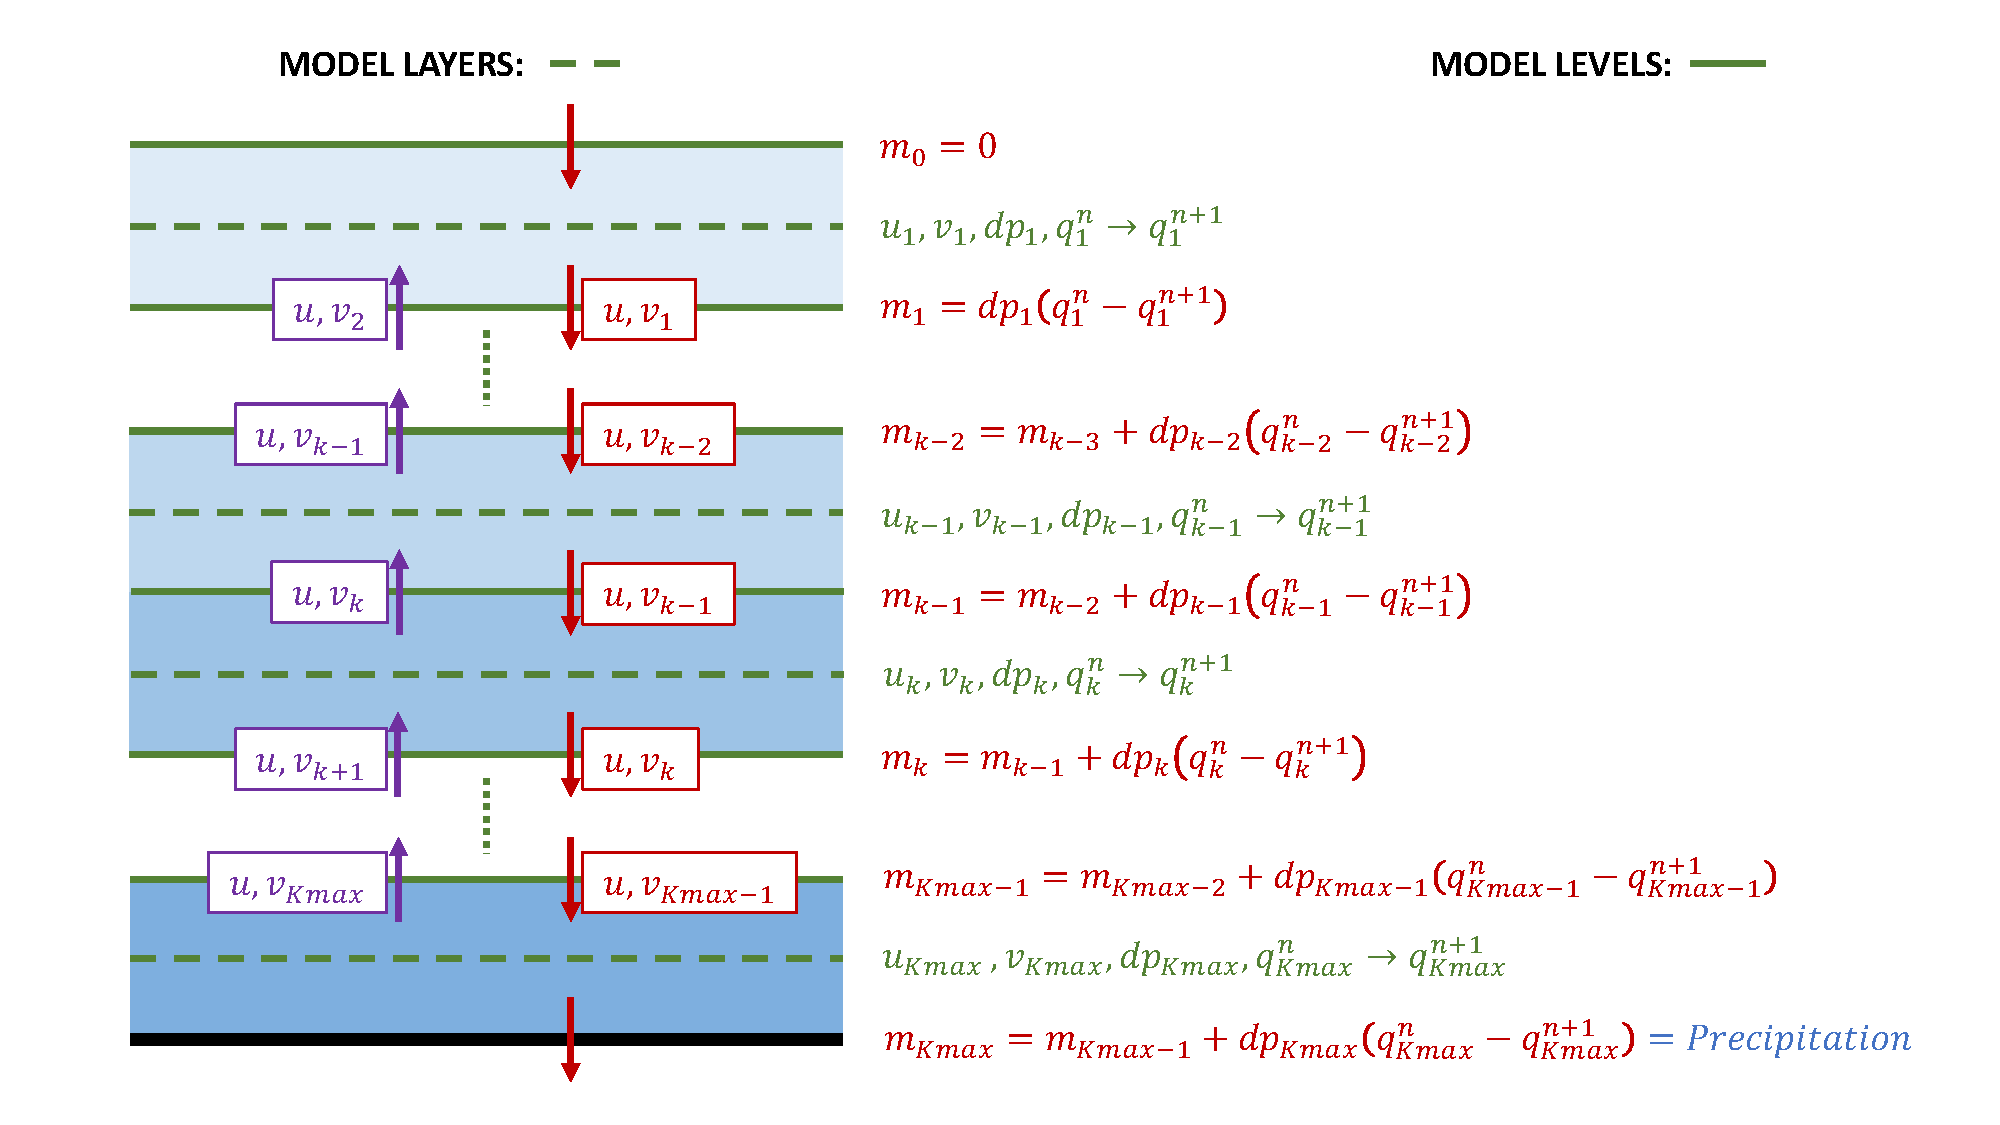
\includegraphics[width=\textwidth]{fig4.pdf}
\caption{Schematic of implicit fall and momentum exchange between the neighbouring layers.}
\label{fig:fig4}
\end{figure}

%------------------------------------------------------------------------------

\subsection{Lagrangian Falls of hydrometeors}

The Lagrangian fall utilizes the same piecewise parabolic method that is used in the FV3 dynamical core's vertically-Lagrangian solver. Details of this method can be found in Chapter 5 of the public FV3 documentation (\url{https://repository.library.noaa.gov/view/noaa/30725}) \citep{harris2021asci}

%------------------------------------------------------------------------------

\subsection{Impact of Sedimentation on Momentum and Temperature}

Momentum is exchanged when hydrometeors fall. In this process, momentum is always conservative. Horizontal and vertical velocity, as well as associated temperature, are updated after cloud microphysics. Meanwhile, the falling hydrometeors bring down the air temperature from the above layer.

%------------------------------------------------------------------------------

\subsubsection*{Horizontal Velocity}

As it is shown in Figure \ref{fig:fig4}, falling of hydrometeors can bring down the wind speed above and bring up the wind speed below as a compensation. Take the zonal wind ($u$) as an example:
\begin{gather}
	u^{n+1}_k \delta p_k = u^n_k \delta p_k + \alpha - \beta
\end{gather}
where the transport of upper-layer wind down ($\alpha$) and transport of present-layer wind up ($\beta$) are written as:
\begin{gather}
	\alpha = m_{k-1} u^{n+1}_{k-1} \\
	\beta = m_{k-1} u^{n+1}_k
\end{gather}
$m_k$ is the combined falling flux of all hydrometeors. Here the time-implicit form is used. This formula also applies to the meridional wind ($v$).

%------------------------------------------------------------------------------

\subsubsection*{Vertical Velocity}

The transportation of vertical wind is more complicated since it is mixed with the sedimentation of hydrometeor itself. Similar to the transport of zonal wind, falling of hydrometeors can bring down the wind speed above and bring up the wind speed below as a compensation:
\begin{gather}
	w^{n+1}_k \delta p_k = w^n_k \delta p_k + \alpha - \beta
\end{gather}
where the transport of upper-layer wind down ($\alpha$) and transport of present-layer wind up ($\beta$) are written as:
\begin{gather}
	\alpha = m_{k-1} w^{n+1}_{k-1} - m_{k-1} V_{k-1} \\
	\beta = m_{k-1} w^{n+1}_k - m_k V_k
\end{gather}
$m_k$ is the falling flux of each hydrometeor. $V$ is the terminal fall velocity of each hydrometeor.

%------------------------------------------------------------------------------

\subsubsection*{Temperature}

Energy transport is used instead of directly temperature transport to ensure energy conservation. Assume the kinetic energy in the falling condensates is negligible compared to the potential energy. Local thermal equilibrium is assumed, and the loss in potential energy is transformed into internal energy (to heat the whole grid box). Backward time-implicit upwind transport scheme is used:
\begin{gather}
	\delta p_k c_{moist,k} T^{n+1}_k = \delta p_k c_{moist,k} T^n_k + \alpha - \beta
\end{gather}
where the transport of upper-layer energy down ($\alpha$) and transport of present-layer energy up ($\beta$) are written as:
\begin{gather}
	\alpha = m_{k-1} c_* T^{n+1}_{k-1} \\
	\beta = m_k c_* T^{n+1}_{k} - \left(m_k - m_{k-1} \right) c_* T^n_k - m_{k-1} g z_k
\end{gather}

%------------------------------------------------------------------------------

\newpage
\section{Diagnostic Output}

%------------------------------------------------------------------------------

\subsection{Cloud Fraction}

Cloud fraction is diagnosed inside the GFDL MP. Four options are available. The first one is originally designed for this cloud microphysics scheme using the subgrid variability. The second one follows \citet{xu1996asem}. The third one follows \citet{park2016arev}. The fourth one follows \citet{gultepe2007clou}.  The first one is the default option in the current cloud microphysics scheme.

%------------------------------------------------------------------------------

\subsubsection*{Option I (GFDL Method)}

This option uses subgrid variability theory and is similar to that in \citet{letrent1991sens}. Cloud water, cloud ice, rain, snow, and graupel are considered for computing cloud fraction. Define a new air temperature, the liquid-frozen water temperature ($T_{in}$), by assuming all liquid-phase water is evaporated to water vapor and all solid-phase water is sublimated to water vapor:
\begin{gather}
	T_{in} = \dfrac{c_{moist} T - L_v \left(q_{liquid} + q_{solid} \right) - L_f \left(q_{ice} + q_{snow} + q_{graupel} \right)}{c_{v,dry} + \left(q_{vapor} + q_{cond} \right) c_{v,vapor}}
\end{gather}
$T_{in}$ then is used to calculate the saturation mass mixing ratio ($q_{sat}$):
\begin{align}
	q_{sat} =
	\begin{cases}
		q_{s2}(T_{in}), & \quad \text{if} \ T_{in} \leq T_{freez} - 40 \\
		q_{sw}(T_{in}), & \quad \text{if} \ T_{in} \geq T_{freez} \\
		\alpha q_{s2}(T_{in}) + \beta q_{sw}(T_{in}), & \quad \text{if} \ T_{freez} - 40 < T_{in} < T_{freez}	\end{cases}
\end{align}
where $\alpha$ and $\beta$ are the partitioning factors defined as:
\begin{align}
	\alpha =&
	\begin{cases}
		\dfrac{q_{solid}}{q_{cond}}, & \quad \text{if} \ q_{cond} > 3 \times 10^{-6} \\[1em]
		\dfrac{T_{freez} - T_{in}}{40}, & \quad \text{if} \ q_{cond} \leq 3 \times 10^{-6}
	\end{cases} \\
	\beta =&
	\begin{cases}
		\dfrac{q_{liquid}}{q_{cond}}, & \quad \text{if} \ q_{cond} > 3 \times 10^{-6} \\[1em]
		1 - \dfrac{T_{freez} - T_{in}}{40}, & \quad \text{if} \ q_{cond} \leq 3 \times 10^{-6}
	\end{cases}
\end{align}
Relative humidity ($RH$) is calculated considering all hydrometeors as they are all assumed to convert to water vapor as:
\begin{gather}
	RH = \dfrac{q_{vapor} + q_{cond}}{q_{sat}}
\end{gather}

When calculating cloud fraction, the subgrid linear distribution in the horizontal ($h_{var}$) is assumed. This is effectively a smoother for the binary cloud scheme. Cloud fraction occurs only when $RH > 0.75$ and $q_{cond} + q_{vapor} > 1 \times 10^{-6}$. The upper and lower bounds of total hydrometeors are written as:
\begin{gather}
	q_{plus} = \left(1 + q_h \right) \left(q_{vapor} + q_{cond} \right) \\
	q_{minus} = \left(1 - q_h \right) \left(q_{vapor} + q_{cond} \right),
\end{gather}
where $q_h$ is as defined in \eqref{eqn:qh}. Finally, the cloud fraction ($CF$) is calculated as:
\begin{align}
	CF =
	\begin{cases}
		1.0, & \quad \text{if}\ q_{sat} < q_{minus} \\
		\dfrac{q_{plus}-q_{sat}}{q_{plus}-q_{minus}}, & \quad \text{if}\ q_{minus} \leq q_{sat} \leq q_{plus}  \\
		0.0, & \quad \text{if}\ q_{sat} > q_{plus}
	\end{cases}
\end{align}

Finally, cloud fraction is constrained by a basic value ($CF_{min}$) and 1.0:
\begin{gather}
	CF = \min \left[1.0 \max \left(CF_{min}, CF \right) \right]
\end{gather}

%------------------------------------------------------------------------------

\subsubsection*{Option II (Xu-Randall Method)}

This option follows \citet{xu1996asem}. It uses the same relative humidity ($RH$), thresholds, saturation mass mixing ratio ($q_{sat}$), and all hydrometeors as option I. Cloud fraction is calculated as:
\begin{align}
	CF = 
	\begin{cases}
		1.0, & \quad \text{if} \ RH \geq 1.0 \\
		RH^{0.25} \left\{1 - \exp \left[- \dfrac{100 q_{cond}}{\left(1 - RH \right)^{0.49} q_{sat}^{0.49}} \right] \right\}, & \quad \text{if} \ 0.65 < RH < 1.0 \\
		0.0, & \quad \text{if} \ RH \leq 0.65
	\end{cases}
\end{align}

%------------------------------------------------------------------------------

\subsubsection*{Option III (Park Method)}

This option follows \citet{park2016arev}. It simply considers the mass mixing ratio of all hydrometeors:
\begin{gather}
	CF' = \dfrac{1}{50} \times \left[5.77 \times \left(100 - \dfrac{x}{1000} \right) \times \left(1000 q_{cond} \right)^{1.07} + 4.82 \times \left(\dfrac{x}{1000} - 50 \right) \times \left(1000 q_{cond} \right)^{0.94} \right]
\end{gather}
Here $CF'$ is the cloud fraction for mixed-phase cloud. It is then adjusted by the ratio of liquid-phase water and solid-phase water:
\begin{gather}
	CF = CF' \left(\dfrac{0.92}{0.96} \dfrac{q_{liquid}}{q_{cond}} + \dfrac{1.0}{0.96} \dfrac {q_{solid}}{q_{cond}} \right)
\end{gather}

%------------------------------------------------------------------------------

\subsubsection*{Option IV (Gultepe-Isaac Method)}

This option follows \citet{gultepe2007clou}. It also simply considers the mass mixing ratio of all hydrometeors:
\begin{align}
	\gamma = \dfrac{1000 q_{cond}}{0.28 + \left(1000 q_{cond} \right)^{0.49}} \\
	CF_{10} = 
	\begin{cases}
		0.0, & \quad \text{if} \ \gamma < 0.18 \\
		- 0.1754 + 0.9811 \gamma - 0.2223 \gamma^2 + 0.0104 \gamma^3, & \quad \text{if} \ 0.18 < \gamma < 2.0 \\
		1.0, & \quad \text{if} \ \gamma > 2.0
	\end{cases} \\
	CF_{100} = 
	\begin{cases}
		0.0, & \quad \text{if} \ \gamma < 0.12 \\
		- 0.0913 + 0.7213 \gamma + 0.1060 \gamma^2 - 0.0946 \gamma^3, & \quad \text{if} \ 0.12 < \gamma < 1.85 \\
		1.0, & \quad \text{if} \ \gamma > 1.85
	\end{cases} \\
	CF = CF_{10} + \left(\log_{10} \dfrac{x}{1000} - 1 \right) \left(CF_{100} - CF_{10} \right)
\end{align}
where $CF_{10}$ is the cloud fraction for 10-km resolution, and $CF_{100}$ is the cloud fraction for 100-km resolution. 

%------------------------------------------------------------------------------

\subsection{Radar Reflectivity}

As it was mentioned in the previous sections, radar reflectivity is the six month of hydrometeor size distribution. Only rain, snow, and graupel, which follow exponential size distribution, are included for radar reflectivity diagnosed. Three radar reflectivity options were built in the GFDL MP. The first one follows \citet{stoelinga2005simu}, the second one follows the revised \citet{stoelinga2005simu} scheme by Smith and Xue \citep{smith1975rada, tong2005ense}. The third one follows \citet{rogers1989asho}. The first one is the default option in the current cloud microphysics scheme.

%------------------------------------------------------------------------------

\subsubsection*{Option I (Stoelinga Method)}

The code to calculate reflectivity was originally from Mark Stoelinga's dbzcalc.f (refer to \url{https://ams.confex.com/ams/32Rad11Meso/techprogram/paper_97032.htm}) from the RIP package, modified for use in the GFDL MP. Rain, snow, and graupel are considered to calculate reflectivity. The reflectivity factor of rain ($f_{rain}$), snow ($f_{snow}$), and graupel ($f_{graupel}$) is defined as
\begin{gather}
	f_{rain} = \gamma \left(\dfrac{1}{\pi \rho_{rain}} \right)^{1.75} 10^{18} \\
	f_{snow} = \alpha \gamma \left(\dfrac{1}{\pi \rho_{snow}} \right)^{1.75} \left(\dfrac{\rho_{snow}}{\rho_{rain}} \right)^2 10^{18} \\
	f_{graupel} = \alpha \gamma \left(\dfrac{1}{\pi \rho_{graupel}} \right)^{1.75} \left(\dfrac{\rho_{graupel}}{\rho_{rain}} \right)^2 10^{18}
\end{gather}
where $\gamma = 720$, $\alpha = 0.224$. If air temperature is higher than $T_{freez}$, compute factor for brightband, where snow or graupel particle scatters like liquid water ($\alpha = 0.224$) because it is assumed to have a liquid skin:
\begin{gather}
	f_{snow} = \dfrac{f_{snow}}{\alpha} \\
	f_{graupel} = \dfrac{f_{graupel}}{\alpha}
\end{gather}
Therefore, the total equivalent reflectivity ($dBZ$) is written as:
\begin{gather}
	dBZ = 10 \log \left\{\max \left[0.01, f_{rain} \dfrac{\left(\rho q_{rain} \right)^{1.75}}{n_{0r}^{0.75}} + f_{snow} \dfrac{\left(\rho q_{snow} \right)^{1.75}}{n_{0s}^{0.75}} + f_{graupel} \dfrac{\left(\rho q_{graupel} \right)^{1.75}}{n_{0g}^{0.75}} \right] \right\}
\end{gather}
Vertically maximum equivalent reflectivity ($dBZ_{max}$) is written as:
\begin{gather}
	dBZ_{max} = \max \left(-20, dBZ \right)
\end{gather}

%------------------------------------------------------------------------------

\subsubsection*{Option II (Smith-Tong-Xue Method)}

This is a modification of the Stoelinga scheme to use parameters from \citet{smith1975rada} and modified by \citet{tong2005ense}, albeit we do not use the modified parameters for the graupel reflectivity. This reflectivity also considers rain, snow and graupel, with snow divided into wet snow and dry snow. The reflectivity factor of rain ($f_{rain}$), wet snow ($f_{snoww}$), dry snow ($f_{snowd}$), and graupel ($f_{graupel}$) is defined as:
\begin{gather}
	f_{rain} = \gamma \left(\dfrac{1}{\pi \rho_{rain}} \right)^{1.75} 10^{18} \\
	f_{snoww} = \gamma \left(\dfrac{1}{\pi \rho_{snow}} \right)^{1.75} 10^{18} \\
	f_{snowd} = \alpha \gamma \left(\dfrac{1}{\pi \rho_{snow}} \right)^{1.75} \left(\dfrac{\rho_{snow}}{\rho_{ice}} \right)^2 10^{18} \\
	f_{graupel} = \gamma \left(\dfrac{1}{\pi \rho_{graupel}} \right)^{1.75} 10^{18}
\end{gather}
where $\gamma = 720$, $\alpha = 0.224$. If air temperature is higher than $T_{freez}$, snow is treated as wet snow because it is assumed to have a liquid skin. If air temperature is lower than $T_{freez}$, snow is treated as dry snow. Therefore, the total equivalent reflectivity ($dBZ$) is written as:
\begin{gather}
	dBZ = 10 \log \left\{\max \left[0.01, f_{rain} \dfrac{\left(\rho q_{rain} \right)^{1.75}}{n_{0r}^{0.75}} + f_{snow} \dfrac{\left(\rho q_{snow} \right)^{1.75}}{n_{0s}^{0.75}} + f_{graupel} \dfrac{\left(\rho q_{graupel} \right)^{1.75}}{n_{0g}^{0.75}} \right] \right\}
\end{gather}
Vertically maximum equivalent reflectivity ($dBZ_{max}$)
\begin{gather}
	dBZ_{max} = \max \left(-20, dBZ \right)
\end{gather}

%------------------------------------------------------------------------------

\subsubsection*{Option III (Rogers-Yau Method)}

This one is follow \cite{rogers1989asho}. Precipitation rate of rain ($Pr_{rain}$), snow ($Pr_{snow}$) and graupel ($Pr_{graupel}$) can be defined as
\begin{gather}
	Pr_{rain} = \dfrac{\rho q}{\rho_{rain}} v_{rain} \\
	Pr_{snow} = \dfrac{\rho q}{\rho_{snow}} v_{snow} \\
	Pr_{graupel} = \dfrac{\rho q}{\rho_{graupel}} v_{graupel}
\end{gather}
Therefore, the total equivalent reflectivity ($dBZ$) is written as:
\begin{gather}
	Z_e = 200 \left[\left(3.6 \times 10^6 Pr_{rain} \right)^{1.6} + \left(3.6 \times 10^6 Pr_{snow} \right)^{1.6} + \left(3.6 \times 10^6 Pr_{graupel} \right)^{1.6} \right] \\
	dbz = 10 \log_{10} \left\{\max \left[0.01, Z_e \right] \right\}
\end{gather}
Vertically maximum equivalent reflectivity ($dBZ_{max}$)
\begin{gather}
	dBZ_{max} = \max \left(-20, dBZ \right)
\end{gather}

%------------------------------------------------------------------------------

\subsection{Cloud Effective Radius}

The cloud effective radius connects the cloud microphysics and radiation. The size and distribution of hydrometeors significantly impact the radiation and the global energy balance. There are several options in the GFDL MP for cloud effective radius calculation. There are also options to decide whether liquid-phase water or solid-phase water should be combined. 

The calculation of effective radius of cloud water ($R_{water}$) has two options. Option one assumes the cloud water is spherical following \citet{martin1994them}:
\begin{gather}
	R_{water} = \left(\dfrac{3 \rho q_{water}}{4 \pi \rho_{water} N_{water}} \right)^{1/3} 10^6
\end{gather}
$N_{water}$ is the empirical number concentration of cloud water following the definition in \citet{martin1994them}. By default, it uses the values of $N_c$ from the GFDL MP. Option two considers the difference of land and ocean, and is simply a function of temperature following revised \citet{kiehl1994sens}:
\begin{gather}
	R'_{water} = 14 (1 - LSM) + \left\{8 + 6 \min \left[1, \max \left(0, \dfrac{T_{freez} - T}{30} \right) \right] \right\} LSM \\
	R_{water} = R'_{water} + \left(14 - R'_{water} \right) \min \left[1, \max \left(0, \dfrac{D_{snow}}{1000} \right) \right]
\end{gather}
where $D_{snow}$ is snow depth.

The calculation effective radius of cloud ice ($R_{ice}$) has five options. Option one is a function of cloud ice content and temperature following \citet{heymsfield1996high}:
\begin{align}
	R_{ice} =
	\begin{cases}
		\dfrac{\beta}{9.917} \left(\rho q_{ice} 10^3 \right)^{0.109} 10^3, & \text{if}\ T < T_0 - 50 \\[1em]
		\dfrac{\beta}{9.337} \left(\rho q_{ice} 10^3 \right)^{0.080} 10^3, & \text{if}\ T_0 - 50 \leq T < T_0 - 40 \\[1em]
		\dfrac{\beta}{9.208} \left(\rho q_{ice} 10^3 \right)^{0.055} 10^3, & \text{if}\ T_0 - 40 \leq T < T_0 - 30 \\[1em]
		\dfrac{\beta}{9.387} \left(\rho q_{ice} 10^3 \right)^{0.031} 10^3, & \text{if}\ T \geq T_0 - 30
	\end{cases},
\end{align}
where $\beta = 1.22$. Option two is simply a function of temperature following \citet{donner1997larg}:
\begin{align}
	R_{ice} =
	\begin{cases}
		15.41627, & \quad \text{if} \ T - T_{freez} < -55 \\
		16.60895, & \quad \text{if} \ -55 \leq T - T_{freez} < -50 \\
		32.89967, & \quad \text{if} \ -50 \leq T - T_{freez} < -45 \\
		35.29989, & \quad \text{if} \ -45 \leq T - T_{freez} < -40 \\
		55.65818, & \quad \text{if} \ -40 \leq T - T_{freez} < -35 \\
		85.19071, & \quad \text{if} \ -35 \leq T - T_{freez} < -30 \\
		72.35392, & \quad \text{if} \ -30 \leq T - T_{freez} < -25 \\
		92.46298, & \quad \text{if} \ T - T_{freez} \ge -25
	\end{cases}
\end{align}
Option three is also a function of temperature following \citet{fu2007anew}:
\begin{gather}
	R_{ice} = 47.05 + 0.6624 \left(T - T_{freez} \right) + 0.001741 \left(T - T_{freez} \right)^2
\end{gather}
Option four is also a function of temperature following \citet{kristjansson2000impa}:
\begin{gather}
	\alpha = \min \left\{ \max \left[(INT \left(T - 136.0 \right), 44 \right], 138 - 1 \right\} \\
	\beta = T - INT(T) \\
	R_{ice} = \Lambda(\alpha) \left(1. - \beta \right) + \Lambda \left(\alpha + 1 \right) \beta
\end{gather}
where $\Lambda$ is a prescribed discrete curve. Option five is a function of cloud ice content and temperature following \citet{wyser1998thee}:
\begin{gather}
	\beta = - 2 + 10^{-3} \times \log_{10} \left(\dfrac{\rho q_{ice}}{\rho_0} \right) \left(T_{freez} - T \right)^{1.5} \\
	R_{ice} = 377.4 + 203.3 \beta + 37.91 \beta^2 + 2.3696 \beta^3
\end{gather}
Option six is a function of cloud ice content and temperature following \citet{sun1999para, sun2001repl}:
\begin{gather}
	R_{ice} = 45.8966 \times \left(\rho q_{ice} 10^3 \right)^{0.2214} + 0.7957 \times \left(\rho q_{ice} 10^3 \right)^{0.2535} \left(T - T_{freez} + 190.0 \right) \\
	R_{ice} = \left[1.2351 + 0.0105 \times \left(T - T_{freez} \right) \right] R_{ice}
\end{gather}

The effective radii of rain ($R_{rain}$), snow ($R_{snow}$), and graupel ($R_{graupel}$) are derived from their size distribution \citet{lin1983bulk}:
\begin{align}
	& R_{rain} = \dfrac{3}{2 \lambda_{rain}} 10^6 \\
	& R_{snow} = \dfrac{3}{2 \lambda_{snow}} 10^6 \\
	& R_{graupel} = \dfrac{3}{2 \lambda_{graupel}} 10^6,
\end{align}
They can also be derived as the mass-weighted form from \citet{lin1983bulk}:
\begin{align}
	& R_{rain} = \dfrac{\left[\dfrac{\Gamma\left(4+b\right)}{6}\right]^{\dfrac{1}{b}}}{2 \lambda_{rain}} 10^6 \\
	& R_{snow} = \dfrac{\left[\dfrac{\Gamma\left(4+d\right)}{6}\right]^{\dfrac{1}{d}}}{2 \lambda_{snow}} 10^6 \\
	& R_{graupel} = \dfrac{\left[\dfrac{\Gamma\left(4+f\right)}{6}\right]^{\dfrac{1}{f}}}{2 \lambda_{graupel}} 10^6,
\end{align}

The maximum and minimum values ($R_{maxrain}$ and $R_{minrain}$, $R_{maxsnow}$ and $R_{minsnow}$, $R_{maxgraupel}$ and $R_{mingraupel}$) are used to cap the range of radii of rain, snow, and graupel.

%------------------------------------------------------------------------------

\newpage

\begin{appendices}

%------------------------------------------------------------------------------

\section{List of Symbols}

\begin{longtable}{p{0.1\textwidth}p{0.5\textwidth}p{0.15\textwidth}p{0.15\textwidth}}
	\hline
	\textbf{Notation}  & \textbf{Description}                                                                 & \textbf{Value}             & \textbf{Units} \\
	\hline
	$a$                & constant in empirical formula                                                        & $842$                      & $cm^{1-b} s^{-1}$ \\
	$a'$               & constant in empirical formula $v_{ice}$                                              & $-4.14122 \times 10^{-5}$  & \\
	$A$                & parameter in sublimation / deposition processes                                      &                            & $s m^{-2}$ \\
	$A'$               & parameter in Bigg mechanism                                                          & $0.66$                     & $K^{-1}$ \\
	$b$                & constant in empirical formula                                                        & $0.8$                      & \\
	$b'$               & constant in empirical formula $v_{ice}$                                              & $-0.00538922$              & \\
	$B$                & parameter in sublimation / deposition processes                                      &                            & $s m^{-2}$ \\
	$B'$               & parameter in Bigg mechanism                                                          & $100$                      & $m^{-3} s^{-1}$ \\
	$c$                & parameter to control snow to cloud water and snow to water vapor conversion          & $4.8$                      & $cm^{1-d} s^{-1}$ \\
	$c'$               & constant in empirical formula $v_{ice}$                                              & $-0.0516344$               & \\
	$c_*$              & heat capacity                                                                        &                            & $J kg^{-1} K^{-1}$ \\
	$c_{moist}$        & moist specific heat                                                                  &                            & $J kg^{-1} K^{-1}$ \\
	$c_{liquid}$       & liquid phase specific heat at $T_{freez}$                                            & $4218$                     & $J kg^{-1} K^{-1}$ \\
	$c_{p,dry}$        & dry air specific heat at constant pressure                                           & $1004.6$                   & $J kg^{-1} K^{-1}$ \\
	$c_{p,liquid}$     & liquid phase specific heat at constant pressure at $T_{freez}$                       & $4218$                     & $J kg^{-1} K^{-1}$ \\
	$c_{p,moist}$      & moist specific heat constant pressure                                                &                            & $J kg^{-1} K^{-1}$ \\
	$c_{p,solid}$      & solid phase specific heat at constant pressure at $T_{freez}$                        & $2106$                     & $J kg^{-1} K^{-1}$ \\
	$c_{p,vapor}$      & water vapor specific heat at constant pressure ($4 R_{vapor}$)                       & $1846$                     & $J kg^{-1} K^{-1}$ \\
	$c_{solid}$        & solid phase specific heat at $T_{freez}$                                             & $2106$                     & $J kg^{-1} K^{-1}$ \\
	$c_{v,dry}$        & dry air specific heat at constant volume ($c_{p,dry} - R_{dry}$)                     & $717.55$                   & $J kg^{-1} K^{-1}$ \\
	$c_{v,liquid}$     & liquid phase specific heat at constant volume at $T_{freez}$                         & $4218$                     & $J kg^{-1} K^{-1}$ \\
	$c_{v,moist}$      & moist specific heat constant volume                                                  &                            & $J kg^{-1} K^{-1}$ \\
	$c_{v,solid}$      & solid phase specific heat at constant volume at $T_{freez}$                          & $2106$                     & $J kg^{-1} K^{-1}$ \\
	$c_{v,vapor}$      & water vapor specific heat at constant volume ($3 R_{vapor}$)                         & $1384.5$                   & $J kg^{-1} K^{-1}$ \\
	$c_{vapor}$        & water vapor specific heat                                                            &                            & $J kg^{-1} K^{-1}$ \\
	$C$                & parameter in evaporation / condensation processes                                    &                            & $s m^{-2}$ \\
	$C_D$              & drag coefficients for hail / graupel                                                 &                            & \\
	$CF$               & cloud fraction                                                                       &                            & \\
	$CF'$              & cloud fraction for mixed-phase cloud                                                 &                            & \\
	$CF_{10}$          & cloud fraction in 10-km resolution                                                   &                            & \\
	$CF_{100}$         & cloud fraction in 100-km resolution                                                  &                            & \\
	$CF_{min}$         & minimum cloud fraction                                                               & $0.05$                     & \\
	$d$                & constant in empirical formula                                                        & $0.25$                     & \\
	$dq$               & difference of hydrometeor mass mixing ratio                                          &                            & $kg kg^{-1}$ \\
	$dp$               & pressure thickness of dry air (positive)                                             &                            & $Pa$ \\
	$dp'$              & pressure thickness of moist air (positive)                                           &                            & $Pa$ \\
	$dt$               & time step                                                                            &                            & $s$ \\
	$dt_c$             & cloud microphysics time step                                                         &                            & $s$ \\
	$dt_{fr}$          & $T_{wfr}$ - $dt_{fr}$: minimum temperature water can exist                           & $8$                        & $K$ \\
	$dt_m$             & vertical remapping time step                                                         &                            & $s$ \\
	$dt_p$             & physics time step                                                                    &                            & $s$ \\
	$dz$               & height thickness (negative)                                                          &                            & $m$ \\
	$dBZ$              & radar reflectivity                                                                   &                            & $dBZ$ \\
	$dBZ_{max}$        & maximum radar reflectivity                                                           &                            & $dBZ$ \\
	$d'$               & constant in empirical formula $v_{ice}$                                              & $0.00216078$               & \\
	$D$                & parameter in evaporation / condensation processes                                    &                            & $s m^{-2}$ \\
	$D_{land}$         & base value for subgrid deviation / variability over land                             & $0.12$                     & $km^{-1/2}$ \\
	$D_{ocean}$        & base value for subgrid deviation / variability over ocean                            & $0.08$                     & $km^{-1/2}$ \\
	$D_{snow}$         & snow depth                                                                           &                            & $m$ \\
	$\bar{D}_{conice}$ & parameter in ice deposition                                                          & $11.9$                     & $m kg^{-0.5}$ \\
	$e$                & constant in empirical formula                                                        & $1$                        & $cm^{1-b} s^{-1}$ \\
	$e'$               & constant in empirical formula $v_{ice}$                                              & $1.9714$                   & \\
	$e_0$              & saturation water vapor pressure at $T_{freez}$                                       & $611.21$                   & $Pa$ \\
	$e_{s0}$           & saturation water vapor pressure for the table N                                      &                            & $Pa$ \\
	$e_{s1}$           & saturation water vapor pressure for the table I                                      &                            & $Pa$ \\
	$e_{s2}$           & saturation water vapor pressure for the table II                                     &                            & $Pa$ \\
	$e_{s3}$           & saturation water vapor pressure for the table III                                    &                            & $Pa$ \\
	$e_{s4}$           & saturation water vapor pressure for the table IV                                     &                            & $Pa$ \\
	$E_{gaci}$         & collection efficiency of cloud ice by graupel                                        & $0.05$                     & \\
	$E_{gacr}$         & collection efficiency of rain by graupel                                             & $1$                        & \\
	$E_{gacs}$         & collection efficiency of snow by graupel                                             & $0.01$                     & \\
	$E_{gacw}$         & collection efficiency of cloud water by graupel                                      & $1$                        & \\
	$E_{racs}$         & collection efficiency of snow by rain                                                & $1$                        & \\
	$E_{racw}$         & collection efficiency of cloud water by rain                                         & $0.8$                      & \\
	$E_{raut}$         & collection efficiency of cloud water to rain autoconversion                          & $0.8$                      & \\
	$E_{saci}$         & collection efficiency of cloud ice by snow                                           &                            & \\
	$E_{sacr}$         & collection efficiency of rain by snow                                                & $1$                        & \\
	$E_{sacw}$         & collection efficiency of cloud water by snow                                         & $1$                        & \\
	$E_{saut}$         & collection efficiency of cloud ice to snow autoconversion                            &                            & \\
	$f$                & constant in empirical formula                                                        & $0.5$                      & \\
	$f_{graupel}$      & reflectivity factor of graupel                                                       &                            & \\
	$f_{rain}$         & reflectivity factor of rain                                                          &                            & \\
	$f_{snow}$         & reflectivity factor of snow                                                          &                            & \\
	$f_{vg}$           & tunable factor for graupel fall                                                      & $1$                        & \\
	$f_{vi}$           & tunable factor for cloud ice fall                                                    & $1$                        & \\
	$f_{vr}$           & tunable factor for rain fall                                                         & $1$                        & \\
	$f_{vs}$           & tunable factor for snow fall                                                         & $1$                        & \\
	$f_{x2y}$          & conversion rate from hydrometeor $x$ to hydrometeor $y$                              &                            & \\
	$g$                & gravitational acceleration                                                           & $9.80665$                  & $m s^{-2}$ \\
	$h_{var}$          & subgrid variability in horizontal direction                                          &                            & \\
	$H$                & Heaviside unit step function                                                         & $0.5$                      & \\
	$IE$               & internal energy                                                                      &                            & $J kg^{-1}$ \\
	$k$                & vertical index                                                                       &                            & \\
	$kbot$             & bottom layer index                                                                   &                            & \\
	$K_a$              & thermal conductivity of air                                                          & $2.36 \times 10^{-2}$      & $J m^{-1} s^{-1} K^{-1}$ \\
	$L$                & latent heat                                                                          &                            & $J kg^{-1}$ \\
	$L_f$              & latent heat of fusion at $0K$                                                        &                            & $J kg^{-1}$ \\
	$L_{fus}$          & latent heat of fusion at $T_{freez}$                                                 & $3.3358 \times 10^5$       & $J kg^{-1}$ \\
	$L_{l2s}$          & true latent heat of melting / freezing                                               &                            & $J kg^{-1}$ \\
	$L_v$              & atent heat of condensation / evaporation at $0K$                                     &                            & $J kg^{-1}$ \\
	$L_{v2l}$          & true latent heat of condensation / evaporation                                       &                            & $J kg^{-1}$ \\
	$L_{v2s}$          & true latent heat of deposition / sublimation                                         &                            & $J kg^{-1}$ \\
	$L_{vap}$          & latent heat of evaporation at $T_{freez}$                                            & $2.5 \times 10^6$          & $J kg^{-1}$ \\
	$L'_{v2l}$         & special latent heat of condensation / evaporation for saturated water vapor          &                            & $J kg^{-1}$ \\
	$LSM$              & land sea mask, 1: land, 0: sea                                                       &                            & \\
	$m$                & sedimentation mass flux                                                              &                            & $Pa$ \\
	$M$                & mass                                                                                 &                            & $kg$ \\
	$M_{dry}$          & dry air mass                                                                         &                            & $kg$ \\
	$M_{graupel}$      & graupel mass                                                                         &                            & $kg$ \\
	$M_{ice}$          & cloud ice mass                                                                       &                            & $kg$ \\
	$M_{rain}$         & rain mass                                                                            &                            & $kg$ \\
	$M_{snow}$         & snow mass                                                                            &                            & $kg$ \\
	$M_{vapor}$        & water vapor mass                                                                     &                            & $kg$ \\
	$M_{water}$        & cloud water mass                                                                     &                            & $kg$ \\
	$n$                & size distribution                                                                    &                            & $m^{-4}$ \\
	$n_0$              & intercept parameter                                                                  &                            & $m^{-4}$ \\
    $n_{graupel}$      & size distribution of graupel                                                         &                            & $m^{-4}$ \\
    $n_{graupel,0}$    & intercept parameter of graupel size distribution                                     & $4.0 \times 10^{6}$        & $m^{-4}$ \\
    $n_{hail}$         & size distribution of hail                                                            &                            & $m^{-4}$ \\
    $n_{hail,0}$       & intercept parameter of hail size distribution                                        & $4.0 \times 10^{4}$        & $m^{-4}$ \\
    $n_{rain}$         & size distribution of rain                                                            &                            & $m^{-4}$ \\
    $n_{rain,0}$       & intercept parameter of rain size distribution                                        & $8.0 \times 10^{6}$        & $m^{-4}$ \\
    $n_{snow}$         & size distribution of snow                                                            &                            & $m^{-4}$ \\
    $n_{snow,0}$       & intercept parameter of snow size distribution                                        & $3.0 \times 10^{6}$        & $m^{-4}$ \\
	$N_c$              & cloud droplet number concentration (CDNC)                                            &                            & $m^{-3}$ \\
	$N_{c,land}$       & prescribed cloud droplet number concentration over land                              & $300$                      & $cm^{-3}$ \\
	$N_{c,ocean}$      & prescribed cloud droplet number concentration over ocean                             & $200$                      & $cm^{-3}$ \\
	$N_{graupel}$      & number concentration of graupel                                                      &                            & $m^{-3}$ \\
	$N_i$              & activated cloud ice number concentration                                             &                            & $m^{-3}$ \\
	$N_{ice}$          & number concentration of cloud ice                                                    &                            & $m^{-3}$ \\
	$N_{rain}$         & number concentration of rain                                                         &                            & $m^{-3}$ \\
	$N_{snow}$         & number concentration of snow                                                         &                            & $m^{-3}$ \\
	$N_{water}$        & number concentration of cloud water                                                  &                            & $m^{-3}$ \\
	$p$                & air pressure                                                                         &                            & $Pa$ \\
	$p_{int}$          & interface air pressure                                                               &                            & $Pa$ \\
	$Pr_{graupel}$     & graupel precipitation rate                                                           &                            & $m s^{-1}$ \\
	$Pr_{rain}$        & rain precipitation rate                                                              &                            & $m s^{-1}$ \\
	$q$                & hydrometeor mass mixing ratio                                                        &                            & $kg kg^{-1}$ \\
	$q'$               & hydrometeor specific ratio                                                           &                            & $kg kg^{-1}$ \\
	$q_{aerosol}$      & aerosol mass mixing ratio                                                            &                            & $kg kg^{-1}$ \\
	$q_{autice}$       & ice to snow density autoconversion threshold                                         & $8 \times 10^{-5}$         & $kg kg^{-3}$ \\
	$q_{autsnow}$      & snow to graupel density autoconversion threshold                                     & $1 \times 10^{-3}$         & $kg kg^{-3}$ \\
	$q_{cond}$         & total water condensate mass mixing ratio                                             &                            & $kg kg^{-1}$ \\
	$q_{crtice}$       & initial ice nuclei mass mixing ratio                                                 &                            & $kg kg^{-1}$ \\
	$q_{crtwater}$     & critical mass mixing ratio for cloud water in autoconversion                         &                            & $kg kg^{-1}$ \\
	$q_{genice}$       & maximum cloud ice generated during remapping step                                    & $1.82 \times 10^{-6}$      & $kg kg^{-1}$ \\
	$q_{genwater}$     & maximum cloud water generated during remapping step                                  & $1 \times 10^{-3}$         & $kg kg^{-1}$ \\
	$q_{graupel}$      & graupel mixing ratio                                                                 &                            & $kg kg^{-1}$ \\
	$q_h$              & dispersion of hydrometeors                                                           &                            & $kg kg^{-1}$ \\
	$q_{hail}$         & hail mixing ratio                                                                    &                            & $kg kg^{-1}$ \\
	$q_{ice}$          & cloud ice mixing ratio                                                               &                            & $kg kg^{-1}$ \\
	$q_{limice}$       & cloud ice limiter to prevent large ice build up                                      & $1$                        & $kg kg^{-1}$ \\
	$q_{liquid}$       & liquid phase water species mass mixing ratio                                         &                            & $kg kg^{-1}$ \\
	$q_{maxice}$       & maximum cloud ice mass mixing ratio for autoconversion of cloud ice                  & $1.0 \times 10^{-4}$       & $kg kg^{-1}$ \\
	$q_{maxwater}$     & maximum cloud water mass mixing ratio for autoconversion of cloud water              & $2 \times 10^{-3}$         & $kg kg^{-1}$ \\
	$q_{mincond}$      & minimum value for cloud condensates                                                  & $1 \times 10^{-12}$        & $kg kg^{-1}$ \\
	$q_{minrain}$      & minimum value for rain                                                               & $1 \times 10^{-8}$         & $kg kg^{-1}$ \\
	$q_{minus}$        & lower bound of the hydrometeors                                                      &                            & $kg kg^{-1}$ \\
	$q_{minvapor}$     & minimum value for water vapor                                                        & $1 \times 10^{-20}$        & $kg kg^{-1}$ \\
	$q_{mltsnow}$      & maximum value of cloud water allowed from melted snow                                & $1 \times 10^{-6}$         & $kg kg^{-1}$ \\
	$q_{mltwater}$     & maximum value of cloud water allowed from melted cloud ice                           & $1 \times 10^{-3}$         & $kg kg^{-1}$ \\
	$q_{plus}$         & upper bound of the hydrometeors                                                      &                            & $kg kg^{-1}$ \\
	$q_{rain}$         & rain mixing ratio                                                                    &                            & $kg kg^{-1}$ \\
	$q_{tmp}$          & a temporal variable to store mass mixing ratio                                       &                            & $kg kg^{-1}$ \\
	$q_s$              & saturation specific humidity for the table I                                         &                            & $kg kg^{-1}$ \\
	$q_{s2}$           & saturation specific humidity for the table III                                       &                            & $kg kg^{-1}$ \\
	$q_{snow}$         & snow mixing ratio                                                                    &                            & $kg kg^{-1}$ \\
	$q_{solid}$        & solid phase water species mass mixing ratio                                          &                            & $kg kg^{-1}$ \\
	$q_{sw}$           & saturation specific humidity for the table II                                        &                            & $kg kg^{-1}$ \\
	$q_{vapor}$        & water vapor mixing ratio                                                             &                            & $kg kg^{-1}$ \\
	$q_{water}$        & cloud water mixing ratio                                                             &                            & $kg kg^{-1}$ \\
	$Q$                & condensates density                                                                  &                            & $kg m^{-3}$ \\
	$r$                & radius of hydrometeor                                                                &                            & $m$ \\
	$r_{thresh}$       & critical cloud drop radius                                                           & $10 \times 10^{-6}$        & $micro$ \\
	$R_{dry}$          & dry air gas constant                                                                 & $287.05$                   & $J kg^{-1} K^{-1}$ \\
	$R_{graupel}$      & graupel radius                                                                       &                            & $micron$ \\
	$R_{ice}$          & cloud ice radius                                                                     &                            & $micron$ \\
	$R_{maxgraupel}$   & maximum graupel radius                                                               &                            & $micron$ \\
	$R_{maxice}$       & maximum cloud ice radius                                                             &                            & $micron$ \\
	$R_{maxrain}$      & maximum rain radius                                                                  &                            & $micron$ \\
	$R_{maxsnow}$      & maximum snow radius                                                                  &                            & $micron$ \\
	$R_{maxwater}$     & maximum cloud water radius                                                           &                            & $micron$ \\
	$R_{mingraupel}$   & minimum graupel radius                                                               &                            & $micron$ \\
	$R_{minice}$       & minimum cloud ice radius                                                             &                            & $micron$ \\
	$R_{minrain}$      & minimum rain radius                                                                  &                            & $micron$ \\
	$R_{minsnow}$      & minimum snow radius                                                                  &                            & $micron$ \\
	$R_{minwater}$     & minimum cloud water radius                                                           &                            & $micron$ \\
	$R_{rain}$         & rain radius                                                                          &                            & $micron$ \\
	$R_{snow}$         & snow radius                                                                          &                            & $micron$ \\
	$R_{vapor}$        & water vapor gas constant                                                             & $461.5$                    & $J kg^{-1} K^{-1}$ \\
	$R_{water}$        & cloud water radius                                                                   &                            & $micron$ \\
	$RH$               & relative humidity                                                                    &                            & \\
	$RH_{adj}$         & relative humidity threshold for complete evaporation / sublimation                   &                            & \\
	$RH_{inc}$         & RH increment for complete evaporation / sublimation of cloud water / cloud ice       & $0.3$                      & \\
	$RH_{inr}$         & RH increment for complete evaporation of rain                                        & $0.3$                      & \\
	$RH_{rain}$        & relative humidity for rain                                                           &                            & \\
	$RH_{revap}$       & relative humidity threshold for rain evaporation                                     &                            & \\
	$S_c$              & Schmidt number $= \nu / \psi$                                                        &                            & \\
	$t$                & time                                                                                 &                            & $s$ \\
	$T$                & air temperature                                                                      &                            & $K$ \\
	$T'$               & scaled air temperature for saturation table                                          &                            & $K$ \\
	$T_{tmp}$          & temporal variable to store air temperature                                           &                            & $K$ \\
	$T_{freez}$        & freezing temperature                                                                 & $273.16$                   & $K$ \\
	$T_{in}$           & liquid frozen temperature                                                            &                            & $K$ \\
	$T_{min}$          & minimum temperature for sublimation of cloud ice                                     & $178$                      & $K$ \\
	$T_{sub}$          & minimum temperature for sublimation of cloud ice                                     & $184$                      & $K$ \\
	$T_{wfr}$          & critical freezing temperature ($T_{freez}$ - 40)                                     & $233.16$                   & $K$ \\
	$T_v$              & virtual temperature                                                                  &                            & $K$ \\
	$u$                & zonal wind                                                                           &                            & $m s^{-1}$ \\
	$v$                & meridional wind                                                                      &                            & $m s^{-1}$ \\
	$v_{gc}$           & constant graupel fall speed                                                          & $2$                        & $m s^{-1}$ \\
	$v_{graupel}$      & graupel fall speed                                                                   &                            & $m s^{-1}$ \\
	$v_{ic}$           & constant cloud ice fall speed                                                        & $1/3$                      & $m s^{-1}$ \\
	$v_{ice}$          & cloud ice fall speed                                                                 &                            & $m s^{-1}$ \\
	$v_{rain}$         & rain fall speed                                                                      &                            & $m s^{-1}$ \\
	$v_{rc}$           & constant rain fall speed                                                             & $4$                        & $m s^{-1}$ \\
	$v_{sc}$           & constant snow fall speed                                                             & $1$                        & $m s^{-1}$ \\
	$v_{snow}$         & snow fall speed                                                                      &                            & $m s^{-1}$ \\
	$v_{maxvg}$        & maximum fall speed for graupel                                                       & $12.0$                     & $m s^{-1}$ \\
	$v_{maxvi}$        & maximum fall speed for cloud ice                                                     & $1.0$                      & $m s^{-1}$ \\
	$v_{maxvr}$        & maximum fall speed for rain                                                          & $12$                       & $m s^{-1}$ \\
	$v_{maxvs}$        & maximum fall speed for snow                                                          & $6.0$                      & $m s^{-1}$ \\
	$v_{minvg}$        & minimum fall speed for graupel                                                       & $1 \times 10^{-5}$         & $m s^{-1}$ \\
	$v_{minvi}$        & minimum fall speed for cloud ice                                                     & $1 \times 10^{-5}$         & $m s^{-1}$ \\
	$v_{minvr}$        & minimum fall speed for rain                                                          & $1 \times 10^{-3}$         & $m s^{-1}$ \\
	$v_{minvs}$        & minimum fall speed for snow                                                          & $1 \times 10^{-5}$         & $m s^{-1}$ \\
	$V$                & terminal velocity                                                                    &                            & $m s^{-1}$ \\
	$w$                & vertical velocity                                                                    &                            & $m s^{-1}$ \\
	$x$                & grid size                                                                            &                            & $m$ \\
	$z$                & height                                                                               &                            & $m$ \\
	$z_{int}$          & interface height                                                                     &                            & $m$ \\
	$z_{var}$          & subgrid variability in vertical direction                                            &                            & \\
	$z_{vir}$          & ratio of the gas constants of dry air and water vapor ($R_{vapor} / R_{dry} - 1$)    & $0.6077338443$             & \\
	$Z_e$              & radar reflectivity factor                                                            &                            & $mm^6 m^{-3} \mu m^3$ \\
	$\chi$             & diffusivity of water vapor in air                                                    & $2.26 \times 10^{-5}$      & $m^2 s^{-1}$ \\
	$\Delta q$         & mass mixing ratio increment                                                          &                            & $kg kg^{-1}$ \\
	$\Delta T$         & temperature increment                                                                &                            & $K$ \\
	$\Gamma$           & gamma function                                                                       &                            & \\
	$\lambda$          & slope parameter                                                                      &                            & $cm^{-1}$ \\
	$\lambda_{graupel}$& slope parameter in graupel size distribution                                         &                            & $cm^{-1}$ \\
	$\lambda_{rain}$   & slope parameter in rain size distribution                                            &                            & $cm^{-1}$ \\
	$\lambda_{snow}$   & slope parameter in snow size distribution                                            &                            & $cm^{-1}$ \\
	$\mu$              & dynamic viscosity of air                                                             & $1.717 \times 10^{-5}$     & $kg m^{-1} s^{-1}$ \\
	$\nu$              & kinematic viscosity of air                                                           & $1.259 \times 10^{-5}$     & $cm^2 s^{-1}$ \\
	$\pi$              & ratio of a circle's circumference to its diameter                                    & 3.1415926535897931         & \\
	$\psi$             & diffusivity of water vapor in air                                                    & $2.11 \times 10^{-5}$      & $cm^2 s^{-1}$ \\
	$\rho$             & air density                                                                          &                            & $kg m^{-3}$ \\
	$\rho_0$           & reference air density                                                                & $1.0$                      & $kg m^{-3}$ \\
	$\rho_{bot}$       & bottom layer air density                                                             &                            & $kg m^{-3}$ \\
	$\rho_{graupel}$   & density of graupel                                                                   & $4 \times 10^2$            & $kg m^{-3}$ \\
	$\rho_{hail}$      & density of hail                                                                      & $9.17 \times 10^2$         & $kg m^{-3}$ \\
	$\rho_{rain}$      & density of rain                                                                      & $1 \times 10^3$            & $kg m^{-3}$ \\
	$\rho_{sfc}$       & surface air density                                                                  & $1.2$                      & $kg m^{-3}$ \\
	$\rho_{snow}$      & density of snow                                                                      & $1 \times 10^2$            & $kg m^{-3}$ \\
	$\rho_{water}$     & density of cloud water                                                               & $1 \times 10^3$            & $kg m^{-3}$ \\
	$\tau_{x2y}$       & relaxation time scale from hydrometeor $x$ to hydrometeor $y$                        &                            & $s$ \\
	\hline
\end{longtable}

%------------------------------------------------------------------------------

\newpage
\section{List of Constants in IFS}

\begin{tabular}{p{0.1\textwidth}p{0.5\textwidth}p{0.15\textwidth}p{0.15\textwidth}}
	\hline
	\textbf{Notation}  & \textbf{Description}                                                                 & \textbf{Value}             & \textbf{Units} \\
	\hline
	$R_E$              & Earth radius                                                                         & $6371229$                  & $m$ \\
	$c_{light}$        & speed of light in vacuum                                                             & $299792458$                & $m s^{-1}$ \\
	$c_{p,dry}$        & dry air specific heat at constant pressure ($7 / 2 R_{dry}$)                         & $1004.7090$                & $J kg^{-1} K^{-1}$ \\
	$c_{p,liquid}$     & liquid phase specific heat at constant pressure at $T_{freez}$                       & $4218$                     & $J kg^{-1} K^{-1}$ \\
	$c_{p,solid}$      & solid phase specific heat at constant pressure at $T_{freez}$                        & $2106$                     & $J kg^{-1} K^{-1}$ \\
	$c_{p,vapor}$      & water vapor specific heat at constant pressure ($4 R_{vapor}$)                       & $1846.1$                   & $J kg^{-1} K^{-1}$ \\
	$c_{v,dry}$        & dry air specific heat at constant volume ($5 / 2 R_{dry}$)                           & $717.6493$                 & $J kg^{-1} K^{-1}$ \\
	$c_{v,liquid}$     & liquid phase specific heat at constant volume at $T_{freez}$                         & $4218$                     & $J kg^{-1} K^{-1}$ \\
	$c_{v,solid}$      & solid phase specific heat at constant volume at $T_{freez}$                          & $2106$                     & $J kg^{-1} K^{-1}$ \\
	$c_{v,vapor}$      & water vapor specific heat at constant volume ($3 R_{vapor}$)                         & $1384.575$                 & $J kg^{-1} K^{-1}$ \\
	$g$                & gravitational acceleration                                                           & $9.80665$                  & $m s^{-2}$ \\
	$h$                & Planck constant                                                                      & $6.6260755 \times 10^{-34}$& $J s$ \\
	$K$                & Boltzmann constant                                                                   & $1.380658 \times 10^{-23}$ & $J K^{-1}$ \\
	$L_{fus}$          & latent heat of fusion at $T_{freez}$                                                 & $3.337 \times 10^5$        & $J kg^{-1}$ \\
	$L_{vap}$          & latent heat of evaporation at $T_{freez}$                                            & $2.5008 \times 10^6$       & $J kg^{-1}$ \\
	$m_{dry}$          & dry air molar mass                                                                   & $28.9644 \times 10^{-3}$   & $kg mol^{-1}$ \\
	$m_{vapor}$        & water vapor molar mass                                                               & $18.0153 \times 10^{-3}$   & $kg mol^{-1}$ \\
	$N$                & Avogadro number                                                                      & $6.0221367 \times 10^{23}$ & $mol^{-1}$ \\
	$R$                & universal gas constant ($N K$)                                                       & $8.31451$                  & $J K^{-1} mol^{-1}$ \\
	$R_{dry}$          & dry air gas constant ($R / m_{dry}$)                                                 & $287.0597$                 & $J kg^{-1} K^{-1}$ \\
	$R_{vapor}$        & water vapor gas constant ($R / m_{vapor}$)                                           & $461.5250$                 & $J kg^{-1} K^{-1}$ \\
	$S_0$              & total solar irradiance                                                               & $1370$                     & $W m^{-2}$ \\
	$T_{freez}$        & freezing temperature                                                                 & $273.16$                   & $K$ \\
	$z_{vir}$          & ratio of the gas constants of dry air and water vapor ($R_{vapor} / R_{dry} - 1$)    & $0.6078$                   & \\
	$\sigma$           & Stefan-Boltzmann constant ($\dfrac{2 \pi^5 K^4}{15 c_{light}^2 h^3}$)                & $5.6705085 \times 10^{-8}$ & $W m^{-2} K^{-4}$ \\
	\hline
\end{tabular}

Data in this table is obtained from the IFS documentation: \url{https://www.ecmwf.int/en/elibrary/18714-ifs-documentation-cy45r1-part-iv-physical-processes}

%------------------------------------------------------------------------------

\newpage
\section{Namelist Guide}
\setlength{\parskip}{0em}

%------------------------------------------------------------------------------

\subsection{General}

\hangindent=2em
\hangafter=1
\textbf{mp\_time}\\ Real: Sub time step of the GFDL MP. If \textbf{mp\_time} isn't divisible by physics time step or is larger than physics time step, the actual MP time step becomes $dt / \text{NINT}[dt / \text{MIN}(dt, mp\_time)]$. The unit is $s$. $150$ by default.

\hangindent=2em
\hangafter=1
\textbf{ntimes}\\ Integer: Sub cycle times in the GFDL MP. It used to divide the remapping time step or physics time step. $1$ by default.

\hangindent=2em
\hangafter=1
\textbf{fix\_negative}\\ Logical: Set $.true.$ to fix negative hydrometeors using other hydrometeors or nearby points. $.true.$ as default.

\hangindent=2em
\hangafter=1
\textbf{consv\_checker}\\ Logical: Set $.true.$ to activate the total energy and total water checker. $.false.$ by default.

%------------------------------------------------------------------------------

\subsection{Conversion Time Scale}

\hangindent=2em
\hangafter=1
\textbf{tau\_v2l}\\ Real: Time scale for cloud water condensation. Increasing / decreasing \textbf{tau\_v2l} can slow down / speed up cloud water condensation (water vapor $\rightarrow$ cloud water). The unit is $s$. $150$ by default.

\hangindent=2em
\hangafter=1
\textbf{tau\_l2v}\\ Real: Time scale for cloud water evaporation. Increasing / decreasing \textbf{tau\_l2v} can slow down / speed up cloud water evaporation (cloud water $\rightarrow$ water vapor). The unit is $s$. $300$ by default.

\hangindent=2em
\hangafter=1
\textbf{tau\_l2r}\\ Real: Time scale for autoconversion of cloud water to rain. Increasing / decreasing \textbf{tau\_l2r} can slow down / speed up autoconversion of cloud water to rain (cloud water $\rightarrow$ rain). The unit is $s$. $900$ by default.

\hangindent=2em
\hangafter=1
\textbf{tau\_r2g}\\ Real: Time scale for freezing of rain to graupel. Increasing / decreasing \textbf{tau\_r2g} can slow down / speed up freezing of rain to graupel (rain $\rightarrow$ graupel). The unit is $s$. $900$ by default.

\hangindent=2em
\hangafter=1
\textbf{tau\_i2s}\\ Real: Time scale for autoconversion of cloud ice to snow. Increasing / decreasing \textbf{tau\_i2s} can slow down / speed up autoconversion of cloud ice to snow (cloud ice $\rightarrow$ snow). The unit is $s$. $1000$ by default.

\hangindent=2em
\hangafter=1
\textbf{tau\_imlt}\\ Real: Time scale for cloud ice melting. Increasing / decreasing \textbf{tau\_imlt} can slow down / speed up melting of cloud ice to cloud water or rain (cloud ice $\rightarrow$ cloud water or rain). The unit is $s$. $1200$ by default.

\hangindent=2em
\hangafter=1
\textbf{tau\_smlt}\\ Real: Time scale for snow melting. Increasing / decreasing \textbf{tau\_smlt} can slow down / speed up melting of snow to cloud water or rain (snow $\rightarrow$ cloud water or rain). The unit is $s$. $900$ by default.

\hangindent=2em
\hangafter=1
\textbf{tau\_gmlt}\\ Real: Time scale for graupel melting. Increasing / decreasing \textbf{tau\_g2r} can slow down / speed up melting of graupel to rain (graupel $\rightarrow$ rain). The unit is $s$. $600$ by default.

\hangindent=2em
\hangafter=1
\textbf{tau\_revp}\\ Real: Time scale for rain evaporation. Increasing / decreasing \textbf{tau\_g2r} can slow down / speed up rain evaporation (rain $\rightarrow$ water vapor). The unit is $s$. $0$ by default.

%------------------------------------------------------------------------------

\subsection{Subgrid Variability}

\hangindent=2em
\hangafter=1
\textbf{dw\_land}\\ Real: Basic value for subgrid variability over land. $0.2$ by default.

\hangindent=2em
\hangafter=1
\textbf{dw\_ocean}\\ Real: Basic value for subgrid variability over ocean. $0.1$ by default.

\hangindent=2em
\hangafter=1
\textbf{z\_slope\_liq}\\ Logical: Set $.true.$ to turn on vertically subgrid linear monotonic slope for autoconversion of cloud water to rain. $.true.$ by default.

\hangindent=2em
\hangafter=1
\textbf{z\_slope\_ice}\\ Logical: Set $.true.$ to turn on vertically subgrid linear monotonic slope for autoconversion of cloud ice to snow. $.true.$ by default.

%------------------------------------------------------------------------------

\subsection{Fall Speed}

\hangindent=2em
\hangafter=1
\textbf{const\_vi}\\ Logical: Set $.true.$ to use constant cloud ice terminal fall velocity. $.false.$ by default.

\hangindent=2em
\hangafter=1
\textbf{const\_vs}\\ Logical: Set $.true.$ to use constant snow terminal fall velocity. $.false.$ by default.

\hangindent=2em
\hangafter=1
\textbf{const\_vg}\\ Logical: Set $.true.$ to use constant graupel terminal fall velocity. $.false.$ by default.

\hangindent=2em
\hangafter=1
\textbf{const\_vr}\\ Logical: Set $.true.$ to use constant rain terminal fall velocity. $.false.$ by default.

\hangindent=2em
\hangafter=1
\textbf{vi\_fac}\\ Real: Scale factor for cloud ice fall or the constant cloud ice terminal fall velocity when \textbf{const\_vi} is $.true.$. The unit is $1$. $1$ by default.

\hangindent=2em
\hangafter=1
\textbf{vr\_fac}\\ Real: Scale factor for rain fall or the constant rain terminal fall velocity when \textbf{const\_vr} is $.true.$. The unit is $1$. $1$ by default.

\hangindent=2em
\hangafter=1
\textbf{vs\_fac}\\ Real: Scale factor for snow fall or the constant snow terminal fall velocity when \textbf{const\_vs} is $.true.$. The unit is $1$. $1$ by default.

\hangindent=2em
\hangafter=1
\textbf{vg\_fac}\\ Real: Scale factor for graupel fall or the constant graupel terminal fall velocity when \textbf{const\_vg} is $.true.$. The unit is $1$. $1$ by default.

\hangindent=2em
\hangafter=1
\textbf{vi\_max}\\ Real: Maximum terminal fall velocity for cloud ice. The unit is $m s^{-1}$. $1$ as default.

\hangindent=2em
\hangafter=1
\textbf{vs\_max}\\ Real: Maximum terminal fall velocity for snow. The unit is $m s^{-1}$. $2$ as default.

\hangindent=2em
\hangafter=1
\textbf{vg\_max}\\ Real: Maximum terminal fall velocity for graupel. The unit is $m s^{-1}$. $12$ as default.

\hangindent=2em
\hangafter=1
\textbf{vr\_max}\\ Real: Maximum terminal fall velocity for rain. The unit is $m s^{-1}$. $12$ as default.

%------------------------------------------------------------------------------

\subsection{Conversion Threshold}

\hangindent=2em
\hangafter=1
\textbf{ql\_mlt}\\ Real: Maximum value of cloud water allowed from melted cloud ice (cloud ice $\rightarrow$ cloud water or rain). Exceed of which will become rain. Increasing / decreasing \textbf{ql\_mlt} can increase / decrease cloud water and decrease / increase rain. The unit is $kg kg^{-1}$. $1.0 \times 10^{-3}$ by default.

\hangindent=2em
\hangafter=1
\textbf{qs\_mlt}\\ Real: Maximum value of cloud water allowed from melted snow (snow $\rightarrow$ cloud water or rain). Exceed of which will become rain. Increasing / decreasing \textbf{qs\_mlt} can increase / decrease cloud water and decrease / increase rain. The unit is $kg kg^{-1}$. $1.0 \times 10^{-6}$ by default.

\hangindent=2em
\hangafter=1
\textbf{ql\_gen}\\ Real: Maximum value for cloud water generated from condensation of water vapor (water vapor $\rightarrow$ cloud water). Increasing / decreasing \textbf{ql\_gen} can increase / decrease cloud water. The unit is $kg kg^{-1}$. $1.0 \times 10^{-3}$ by default.

\hangindent=2em
\hangafter=1
\textbf{ql0\_max}\\ Real: Threshold of cloud water to rain autoconversion (cloud water $\rightarrow$ rain). Increasing / decreasing \textbf{ql0\_max} can increase / decrease cloud water and decrease / increase rain. The unit is $kg kg^{-1}$. $2.0 \times 10^{-3}$ by default.

\hangindent=2em
\hangafter=1
\textbf{qi0\_max}\\ Real: Maximum value of cloud ice generated from other sources like convection. Exceed of which will become snow. Increasing / decreasing \textbf{qi0\_max} can increase / decrease cloud ice and decrease / increase snow. The unit is $kg kg^{-1}$. $1.0 \times 10^{-4}$ by default.

\hangindent=2em
\hangafter=1
\textbf{qi0\_crt}\\ Real: Threshold of cloud ice to snow autoconversion (cloud ice $\rightarrow$ snow). Increasing / decreasing \textbf{qi0\_crt} can increase / decrease cloud ice and decrease / increase snow. The unit is $kg m^{-3}$. $8 \times 10^{-5}$ by default.

\hangindent=2em
\hangafter=1
\textbf{qs0\_crt}\\ Real: Threshold of snow to graupel autoconversion (snow $\rightarrow$ graupel). Increasing / decreasing \textbf{qs0\_crt} can increase / decrease snow and decrease / increase graupel. The unit is $kg m^{-3}$. $1.0 \times 10^{-3}$ by default.

\hangindent=2em
\hangafter=1
\textbf{qi\_lim}\\ Real: Cloud ice limiter to prevent ice built up in cloud ice freezing (cloud water $\rightarrow$ cloud ice) and deposition (water vapor $\rightarrow$ cloud ice). The unit is $1$. $1$ by default.

\hangindent=2em
\hangafter=1
\textbf{rh\_inc}\\ Real: Relative humidity increment for complete evaporation of cloud water and cloud ice. The unit is $1$. $0.3$ by default.

\hangindent=2em
\hangafter=1
\textbf{rh\_ins}\\ Real: Relative humidity increment for minimum evaporation of rain. The unit is $1$. $0.3$ by default.

\hangindent=2em
\hangafter=1
\textbf{rh\_inr}\\ Real: Relative humidity increment for rain evaporation. The unit is $1$. $0.3$ by default.

\hangindent=2em
\hangafter=1
\textbf{rthresh}\\ Real: Critical cloud water radius for autoconversion (cloud water $\rightarrow$ rain). Increasing / decreasing of \textbf{rthresh} can slow down / speed up the autoconversion. The unit is $mm$. $1.0 \times 10^{-5}$ by default.

%------------------------------------------------------------------------------

\subsection{Conversion Efficiency}

\hangindent=2em
\hangafter=1
\textbf{c\_pracw}\\ Real: Accretion efficiency of cloud water to rain (cloud water $\rightarrow$ rain). Increasing / decreasing of \textbf{c\_pracw} can speed up / slow down the accretion of cloud water by rain. The unit is $1$. $0.9$ by default.

\hangindent=2em
\hangafter=1
\textbf{c\_psacw}\\ Real: Accretion efficiency of cloud water to snow (cloud water $\rightarrow$ snow). Increasing / decreasing of \textbf{c\_psacw} can speed up / slow down the accretion of cloud water by snow. The unit is $1$. $1$ by default.

\hangindent=2em
\hangafter=1
\textbf{c\_pgacw}\\ Real: Accretion efficiency of cloud water to graupel (cloud water $\rightarrow$ graupel). Increasing / decreasing of \textbf{c\_pgacw} can speed up / slow down the accretion of cloud water by graupel. The unit is $1$. $1$ by default.

\hangindent=2em
\hangafter=1
\textbf{c\_psaci}\\ Real: Accretion efficiency of cloud ice to snow (cloud ice $\rightarrow$ snow). Increasing / decreasing of \textbf{c\_psaci} can speed up / slow down the accretion of cloud ice by snow. The unit is $1$. $0.02$ by default.

\hangindent=2em
\hangafter=1
\textbf{c\_pgaci}\\ Real: Accretion efficiency of cloud ice to graupel (cloud ice $\rightarrow$ graupel). Increasing / decreasing of \textbf{c\_pgaci} can speed up / slow down the accretion of cloud ice by graupel. The unit is $1$. $0.05$ by default.

\hangindent=2em
\hangafter=1
\textbf{c\_praci}\\ Real: Accretion efficiency of cloud ice to rain (cloud ice $\rightarrow$ rain). Increasing / decreasing of \textbf{c\_praci} can speed up / slow down the accretion of cloud ice by rain. The unit is $1$. $1$ by default.

\hangindent=2em
\hangafter=1
\textbf{c\_pgacs}\\ Real: Accretion efficiency of snow to graupel (snow $\rightarrow$ graupel). Increasing / decreasing of \textbf{c\_pgacs} can speed up / slow down the accretion of snow by graupel. The unit is $1$. $0.01$ by default.

\hangindent=2em
\hangafter=1
\textbf{c\_pracs}\\ Real: Accretion efficiency of snow to rain (snow $\rightarrow$ rain). Increasing / decreasing of \textbf{c\_pracs} can speed up / slow down the accretion of snow by rain. The unit is $1$. $1$ by default.

\hangindent=2em
\hangafter=1
\textbf{c\_psacr}\\ Real: Accretion efficiency of rain to snow (rain $\rightarrow$ snow). Increasing / decreasing of \textbf{c\_psacr} can speed up / slow down the accretion of rain by snow. The unit is $1$. $1$ by default.

\hangindent=2em
\hangafter=1
\textbf{c\_pgacr}\\ Real: Accretion efficiency of rain to graupel (rain $\rightarrow$ graupel). Increasing / decreasing of \textbf{c\_pgacr} can speed up / slow down the accretion of rain by graupel. The unit is $1$. $1$ by default.

\hangindent=2em
\hangafter=1
\textbf{c\_paut}\\ Real: Autoconversion efficiency of cloud water to rain (cloud water $\rightarrow$ rain). Increasing / decreasing of \textbf{c\_paut} can speed up / slow down the autoconversion of cloud water to rain.  The unit is $1$. $0.5$ by default.

%------------------------------------------------------------------------------

\subsection{Options}

\hangindent=2em
\hangafter=1
\textbf{cfflag}\\ Cloud fraction scheme. 1: GFDL cloud scheme; 2: \citet{xu1996asem}; 3: \citet{park2016arev}; 4: \citet{gultepe2007clou}. $1$ by default.

\hangindent=2em
\hangafter=1
\textbf{icloud\_f}\\ GFDL cloud scheme. 0: subgrid variability based scheme; 1: same as 0, but for old fvgfs implementation; 2: binary cloud scheme; 3: extension of  0. $0$ by default.

\hangindent=2em
\hangafter=1
\textbf{irain\_f}\\ Cloud water to rain auto conversion scheme. 0: subgrid variability based scheme; 1: no subgrid varaibility. $0$ by default.

\hangindent=2em
\hangafter=1
\textbf{inflag}\\ Ice nucleation scheme. 1: \citet{hong2004arev}; 2: \citet{meyers1992newp}; 3: \citet{meyers1992newp}; 4: \citet{cooper1986icei}; 5: \citet{fletcher1962thep}. $1$ by default.

\hangindent=2em
\hangafter=1
\textbf{igflag}\\ Ice generation scheme. 1: WSM6; 2: WSM6 with 0 at 0 C; 3: WSM6 with 0 at 0 C and fixed value at - 10 C; 4: combination of 1 and 3. $3$ by default.

\hangindent=2em
\hangafter=1
\textbf{ifflag}\\ Ice fall scheme. 1: \citet{deng2008cirr}; 2: \citet{heymsfield1990asch}. $1$ by default.

\hangindent=2em
\hangafter=1
\textbf{rewflag}\\ Cloud water effective radius scheme. 1: \citet{martin1994them}; 2: \citet{martin1994them}, GFDL revision; 3: \citet{kiehl1994sens}. $1$ by default.

\hangindent=2em
\hangafter=1
\textbf{reiflag}\\ Cloud water effective radius scheme. 1: \citet{heymsfield1996high}; 2: \citet{donner1997larg}; 3: \citet{fu2007anew}; 4: \citet{kristjansson2000impa}; 5: \citet{wyser1998thee}; 6: \citet{sun1999para, sun2001repl}. $5$ by default.

\hangindent=2em
\hangafter=1
\textbf{rerflag}\\ Rain effective radius scheme. 1: effective radius; 2: mass-weighted effective radius. $1$ by default.

\hangindent=2em
\hangafter=1
\textbf{resflag}\\ Snow effective radius scheme. 1: effective radius; 2: mass-weighted effective radius. $1$ by default.

\hangindent=2em
\hangafter=1
\textbf{regflag}\\ Graupel effective radius scheme. 1: effective radius; 2: mass-weighted effective radius. $1$ by default.

\hangindent=2em
\hangafter=1
\textbf{radr\_flag}\\ Radar reflectivity for rain. 1: \citet{stoelinga2005simu}; 2: \citet{smith1975rada, tong2005ense}; 3: Marshall-Palmer formula (\url{https://en.wikipedia.org/wiki/DBZ_(meteorology)}). $1$ by default.

\hangindent=2em
\hangafter=1
\textbf{rads\_flag}\\ Radar reflectivity for snow. 1: \citet{stoelinga2005simu}; 2: \citet{smith1975rada, tong2005ense}; 3: Marshall-Palmer formula (\url{https://en.wikipedia.org/wiki/DBZ_(meteorology)}). $1$ by default.

\hangindent=2em
\hangafter=1
\textbf{radg\_flag}\\ Radar reflectivity for graupel. 1: \citet{stoelinga2005simu}; 2: \citet{smith1975rada, tong2005ense}; 3: Marshall-Palmer formula (\url{https://en.wikipedia.org/wiki/DBZ_(meteorology)}). $1$ by default.

\hangindent=2em
\hangafter=1
\textbf{do\_hail}\\ Logical: Set $.true.$ to change all graupel properties to hail properties so that graupel becomes hail. $.false.$ by default.

\hangindent=2em
\hangafter=1
\textbf{do\_cond\_timescale}\\ Logical: Set $.true.$ to scale cloud water condensation to make it slower. $.false.$ by default.

\hangindent=2em
\hangafter=1
\textbf{use\_rhc\_cevap}\\ Logical: Set $.true.$ to reduce evaporation / condensation by adding a cap. $.false.$ by default.

\hangindent=2em
\hangafter=1
\textbf{use\_rhc\_revap}\\ Logical: Set $.true.$ to reduce evaporation / condensation by adding a relative humidity threshold. $.false.$ by default.

\hangindent=2em
\hangafter=1
\textbf{liq\_ice\_combine}\\ Logical: Set $.true.$ to combine all liquid water, combine all solid water in cloud effective radius diagnostic. $.false.$ by default.

\hangindent=2em
\hangafter=1
\textbf{snow\_grauple\_combine}\\ Logical: Set $.true.$ to combine snow and graupel in cloud effective radius diagnostic. $.true.$ by default.

\hangindent=2em
\hangafter=1
\textbf{do\_warm\_rain\_mp}\\ Logical: Set $.true.$ to do warm rain microphysics only. It removes all ice microphysics processes. $.false.$ by default.

%------------------------------------------------------------------------------

\subsection{Cloud Fraction}

\hangindent=2em
\hangafter=1
\textbf{do\_qa}\\ Logical: Set $.true.$ to activate cloud fraction diagnosis. $.true.$ as default.

\hangindent=2em
\hangafter=1
\textbf{rad\_rain}\\ Logical: Set $.true.$ to consider rain in cloud fraction calculation. $.true.$ by default.

\hangindent=2em
\hangafter=1
\textbf{rad\_snow}\\ Logical: Set $.true.$ to consider snow in cloud fraction calculation. $.true.$ by default.

\hangindent=2em
\hangafter=1
\textbf{rad\_graupel}\\ Logical: Set $.true.$ to consider graupel in cloud fraction calculation. $.true.$ by default.

\hangindent=2em
\hangafter=1
\textbf{do\_cld\_adj}\\ Logical: Set $.true.$ to adjust cloud fraction based on the \citet{xu1996asem} scheme. $.false.$ by default.

\hangindent=2em
\hangafter=1
\textbf{cld\_min}\\ Real: Minimum cloud fraction. If total cloud condensate exceeds $1 \times 10^{-6} kg kg^{-1}$, cloud fraction cannot be less than \textbf{cld\_min}. The unit is $1$. $0.05$ by default.

\hangindent=2em
\hangafter=1
\textbf{xr\_a}\\ Real: p value in \citet{xu1996asem}. $0.25$ by default.

\hangindent=2em
\hangafter=1
\textbf{xr\_b}\\ Real: alpha\_0 value in \citet{xu1996asem}. $100$ by default.

\hangindent=2em
\hangafter=1
\textbf{xr\_c}\\ Real: gamma value in \citet{xu1996asem}. $0.49$ by default.

%------------------------------------------------------------------------------

\subsection{Sedimentation}

\hangindent=2em
\hangafter=1
\textbf{use\_ppm}\\ Logical: Set $.true.$ to use PPM fall scheme. $.false.$ to use time-implicit monotonic fall scheme. $.false.$ by default.

\hangindent=2em
\hangafter=1
\textbf{mono\_prof}\\ Logical: Set $.true.$ to turn on terminal fall with monotonic PPM scheme. This is used together with \textbf{use\_ppm} = $.true.$. $.true.$ by default.

\hangindent=2em
\hangafter=1
\textbf{do\_sedi\_uv}\\ Logical: Set $.true.$ to turn on horizontal momentum transport during sedimentation. $.true.$ by default.

\hangindent=2em
\hangafter=1
\textbf{do\_sedi\_w}\\ Logical: Set $.true.$ to turn on vertical motion transport during sedimentation. $.true.$ by default.

\hangindent=2em
\hangafter=1
\textbf{do\_sedi\_heat}\\ Logical: Set $.true.$ to turn on heat transport during sedimentation. $.true.$ by default.

\hangindent=2em
\hangafter=1
\textbf{do\_sedi\_melt}\\ Logical: Set $.true.$ to turn on cloud ice, snow, and graupel melting during sedimentation. $.true.$ by default.

%------------------------------------------------------------------------------

\subsection{CCN}

\hangindent=2em
\hangafter=1
\textbf{prog\_ccn}\\ Logical: Set $.true.$ to activate prognostic CCN. $.false.$ by default.

\hangindent=2em
\hangafter=1
\textbf{ccn\_l}\\ Real: Base CCN over land. Increasing / decreasing \textbf{ccn\_l} can slow down / speed up the autoconversion of cloud water to rain (cloud water $\rightarrow$ rain). The unit is $cm^{-3}$. $270$ by default.

\hangindent=2em
\hangafter=1
\textbf{ccn\_o}\\ Real: Base CCN over ocean. Increasing / decreasing \textbf{ccn\_o} can slow down / speed up the autoconversion of cloud water to rain (cloud water $\rightarrow$ rain). The unit is $cm^{-3}$. $90$ by default.

%------------------------------------------------------------------------------

\subsection{Others}

\hangindent=2em
\hangafter=1
\textbf{tice\_mlt}\\ Real: Melting temperature. The unit is $K$. $273.16$ by default.

\hangindent=2em
\hangafter=1
\textbf{alin}\\ Real: Parameter $a$ in \citet{lin1983bulk}. Constant in empirical formula for $U_R$. Increasing / decreasing \textbf{alin} can boost / decrease accretion of cloud water by rain (cloud water $\rightarrow$ rain) and rain evaporation (rain $\rightarrow$ water vapor). The unit is $cm^{1-b} s^{-1}$. $842$ by default. This value follows \citet{hong2006thew}.

\hangindent=2em
\hangafter=1
\textbf{blin}\\ Real: Parameter $b$ in \citet{lin1983bulk}.The unit is $1$. $0.8$ by default.

\hangindent=2em
\hangafter=1
\textbf{clin}\\ Real: Parameter $c$ in \citet{lin1983bulk}. Constant in empirical formula for $U_S$. Increase / decreasing \textbf{clin} can boost / decrease accretion of cloud water by snow (cloud water $\rightarrow$ snow), accretion of cloud ice by snow (cloud ice $\rightarrow$ snow), snow sublimation and deposition (snow $\leftrightarrow$ water vapor), and snow melting (snow $\rightarrow$ cloud water or rain). The unit is $cm^{1-d} s^{-1}$. $4.8$ by default.

\hangindent=2em
\hangafter=1
\textbf{dlin}\\ Real: Parameter $d$ in \citet{lin1983bulk}.The unit is $1$. $0.25$ by default.

\hangindent=2em
\hangafter=1
\textbf{elin}\\ Real: Parameter $e$ in \citet{lin1983bulk}. Constant in empirical formula for $U_G$. Increase / decreasing \textbf{elin} can boost / decrease accretion of cloud water by graupel (cloud water $\rightarrow$ graupel), accretion of cloud ice by graupel (cloud ice $\rightarrow$ graupel), graupel sublimation and deposition (graupel $\leftrightarrow$ water vapor), and graupel melting (graupel $\rightarrow$ cloud water or rain). The unit is $cm^{1-d} s^{-1}$. $1$ by default.

\hangindent=2em
\hangafter=1
\textbf{flin}\\ Real: Parameter $f$ in \citet{lin1983bulk}.The unit is $1$. $0.5$ by default.

\hangindent=2em
\hangafter=1
\textbf{t\_min}\\ Real: Temperature threshold for instant deposition. Deposit all water vapor to cloud ice (water vapor $\rightarrow$ cloud ice) when temperature is lower than \textbf{t\_min}. The unit is $K$. $178$ by default.

\hangindent=2em
\hangafter=1
\textbf{t\_sub}\\ Real: Temperature threshold for sublimation. Cloud ice, snow or graupel stops / starts sublimation (cloud ice $\rightarrow$ water vapor, snow $\rightarrow$ water vapor, graupel $\rightarrow$ water vapor) when temperature is lower / higher than \textbf{t\_sub}. The unit is $K$. $184$ by default.

\hangindent=2em
\hangafter=1
\textbf{te\_err}\\ Real: Use in total energy and total water checker. 64bit: $1 \times 10^{-14}$, 32bit: $1 \times 10^{-7}$; turn off to save computer time. $1 \times 10^{-14}$ by default.

%------------------------------------------------------------------------------

\newpage
\section{Document Update Record}

\begin{itemize}
	\setlength\itemsep{0em}
	\item 2022.07.01 Document version 4.0: Used GFDL MP as a short name for "GFDL single-moment five-category cloud microphysics scheme". Clarify the 3rd latent heat coefficient, horizontal subgrid variability, particle size distribution, cloud fraction and radar reflectivity, and cloud drop number concentration. Made some corrections to the saturated specific humidity. Updated GitHub information. Updated the features subsection. Cleaned up the microphysical processes section. Removed unused figures.
	\item 2021.10.09 Document version 3.1: some updates to the introduction section.
	\item 2021.02.16 Document version 3.0: the whole document was overwritten because the whole code was overwritten.
	\item 2019.10.30 Document version 2.3: title changed, more references were included, revised many places to correctly represent the size distribution, and mentioned the plan to develop the double-moment scheme.
	\item 2019.10.14 Document version 2.2: minor update to the number concentration of cloud ice.
	\item 2019.09.06 Document version 2.1: added a reference to cloud fraction scheme I, updated basic equations, removed some red text that has been implemented into the code, updated some formulas, updated the List of Symbols.
	\item 2019.08.28 Document version 2.0: revised the whole document based on the latest version of the GFDL MP.
	\item 2017.10.16 Document version 1.1: updated authors' affiliations, corrected snow melting equation in fast saturation adjustment, added namelist guide.
	\item 2017.07.25 Document version 1.0: adjusted the line spacing, updated author list.
	\item 2017.07.22 Document version 0.7: updated figure 2, updated appendix A and B, revised the CNN formula, added Figure 3,5,6. The whole document has been revised. 
	\item 2017.06.02 Document version 0.6: added distribution declaration, cleaned up main text and formulas, enriched the description of the formulas and included their source and derivation method, fixed some errors, revised the appendix tables, updated the constants and tuning parameters, updated figure \ref{fig:fig1}
	\item 2017.01.31 Document version 0.5: updated some parameters (according to gfdl\_mp\_dev branch), fixed some errors in the formulas and units, added the comparison to IFS constants.
	\item 2016.11.17 Document version 0.4: revised according to code change (according to gfdl\_mp branch), completed radius diagnosis.
	\item 2016.11.04 Document version 0.3: revised the title page, added the references of formulas, corrected several errors, added a new section called reflectivity diagnosis, a new section called Lagrangian falls of hydrometeors.
	\item 2016.10.28 Document version 0.2: added contents, source / sink flow chart, references, basic equations, unified the name of source / sink terms, added a new section called interaction with convection and radiation, a new appendix section called some cloud microphysics parameters, acknowledgment, revised the whole document, corrected the errors, those are not consistent with the code are marked as red color.
	\item 2016.10.20 Document version 0.1: first draft, mainly listing all equations / processes in the GFDL cloud microphysics scheme.
	\item 2016.10.14 Document version 0.0: initiated this document.
\end{itemize}

\end{appendices}

%------------------------------------------------------------------------------

\section*{Acknowledgement}
\addcontentsline{toc}{section}{\protect\numberline{}Acknowledgement}

This document cannot be finished without the huge support from the original developer of GFDL MP, Shian-Jiann Lin. Thank everyone in the FV3 team for using, improving, and criticizing the cloud microphysics scheme in his / her applications, especially Baoqiang Xiang, Xi Chen, Mingjing Tong, Kun Gao, and Kai-Yuan Cheng. We also thank Steve Garner for providing the original version of this cloud microphysics scheme in ZETAC. Special thanks also goes to Songmiao Fan and Huan Guo for reviewing this document and providing their insightful comments.

%------------------------------------------------------------------------------

\section*{Code, Copyright, and Citation}
\addcontentsline{toc}{section}{\protect\numberline{}Code, Copyright, and Citation}

The source code of this document is available on GitHub (\url{https://github.com/linjiongzhou/GFDL-MP}). The source code of the GFDL MP is also available on GitHub in the FV3 repository (\url{https://github.com/NOAA-GFDL/GFDL_atmos_cubed_sphere/}).

%------------------------------------------------------------------------------

\addcontentsline{toc}{section}{References}

\bibliographystyle{ametsoc2014}
\bibliography{GFDL_MP.bib}

%------------------------------------------------------------------------------

\end{document}
